\documentclass[10pt,a4paper,russian,openany]{book}
\usepackage[T2A]{fontenc}
\usepackage[koi8-r]{inputenc}
\usepackage[russian]{babel}

\ifx\pdfoutput\undefined
\usepackage[dvips]{graphicx}
\else
\usepackage{pslatex,pscyr}
\usepackage[pdftex]{graphicx}
\pdfinfo
  { /Title (Training of sportsman - skydivers)
    /Author (Pavel Bashinsky <faust@yalta.net.ua>)
    /Subject (Training of sportsman - skydivers. Guskov A.S.)
    /Keywords (sport,skydive,skydive in USSR,history,D-1-5-Y,D-1-5-U,YT-15,UT-15)
}
\fi

\usepackage{fancyhdr}
\pagestyle{fancy}
\renewcommand{\chaptermark}[1]{\markboth{#1}{}}
\renewcommand{\sectionmark}[1]{\markright{\thesection\ #1}}
\fancyhf{}
\fancyhead[LE,RO]{\thepage\bfseries}
\fancyhead[LO]{\it\rightmark}
\fancyhead[RE]{\leftmark}
\fancypagestyle{plain}{}
\renewcommand{\headrulewidth}{0.5pt}
\renewcommand{\footrulewidth}{0pt}

\newcommand{\idx}[1]{\mbox{\scriptsize #1}}

\topmargin=5pt
\textheight=620pt

\begin{document}
\begin{titlepage}
\begin{center}
{\large �. �. �������}\\
\end{center}
\vspace*{\stretch{1}}

\begin{center}
{\LARGE\bf 
\begin{tabular}{c}
\hline
\\
����������\\[2ex]
����������~--\\[2ex]
�����������\\[2ex]
\hline
\end{tabular}
}
\end{center}
\vspace*{\stretch{2}}

\begin{center}
\small ������\\
������ {\large\flqq}����� ������{\large\frqq}\\
������������ ������ ����\\
1979
\end{center}
\end{titlepage}

\thispagestyle{empty}
\vspace*{\stretch{1}}
{\it
� ����� \flqq���������� ����������-�����������\frqq{} �������������� �� �������
�������� �����������, ���������� � �������� ������� ����������� � ������������
��������� ��-15, �-1-5-�, �-5. ��������������� ������������� ������� ������ �
���������, �������� ���������� �����������, ������������� ���������� �������
� ��������� � �������� \flqq�������� �� ���������� � ���������-������������
���������� ������� ������\frqq{} (�., ���-�� ������, 1974).

����� ���������� �� ������� ���� �����������-������������, ����������
���������� � ������ ������� ����������� ������� � ����������� ������������
������ � ������ ����������, �������������� ���������� �����. �� �����
������������ ����������� ����������� ����������� ������ ��� ����������
������������.
}
\vspace*{\stretch{2}}

\centerline{\copyright~������������ ����� ����, 1979 �.}
\newpage

\pagenumbering{arabic}
\chapter{������� �����������}

\section{�������� ��������}

������� ����������� ������ � �������� �������� �� �����, ������ �� ������
�������� XV~--- ������ XVI ����, � ����� �� ����� ��������� ��� ��������
��������������, ��� ������ �������� ������� ���� �� ���������� �� ����� �
����� ������, �� ����������� ��� ���� ������� ���������. ��������� �� �����
������� ������� �� ��������~--- � 1519 ���� �� ����. ����, �����������
�������� �� �����, ������ ����� �� ������������ � �����.

������ ��� ��� ����������� ������ ����� �������� � ����� �����
\flqq� �������\frqq{} ��� �������� �������� ��� ������ �������� � ������ ��
�����, ������� � ��������� �������� �� �����. ������� �������� ���� � ���,
��� ������� �.~�������� ���� ������� ������, � � ����������������� ��������
�������� �� ����� ������ ������� �� ����. ��� �������� �������, ����
�������� �� ����� ���� ����� ���������.

� 1617 ���� �.~�������� �������� �� ����������������� �� ���������� ������
� ��������� ����� � ������������ �����������.

� 20-� ����� XVII ���� ����������� � �������� ������� ����� ����� ������.
�� ��������� �� ������ ������ �������� ������� ���������, �� ���������
�������� ��������� ������� � �������� �� �������� ���. �������� � ����
��������������� ������ �� ����� ��������, ����� ������������ ����������� �
����������� ����� ����. �� ������ �������� ������� � ��������� �������
����������� ������� � ��������. ���� �� ����� � ������ �������� �� ����� �
������ ��������, �������� �����������.

� 1777 ���� ����������� ������ ������� �������������� � ��������� ��������
����, ����� ��������������� ��� ������ �������� � ������ �� �����. ����������
������ ���������� �� ��������� �������������� � �������� ����� ���� �����.
� ������ �������� ������ ��� ������� ��������� �����. �.~����� �������� �
���� ������ ������ � ����� �������� ����� � ������������ �����������.

����� �������� ���� �������� ����������� ������ �������� � ������ �� �����,
�� ������������ ���������� ��� ���� ����� ���� � ���������� ��������� �����.

\begin{figure}
    \centerline{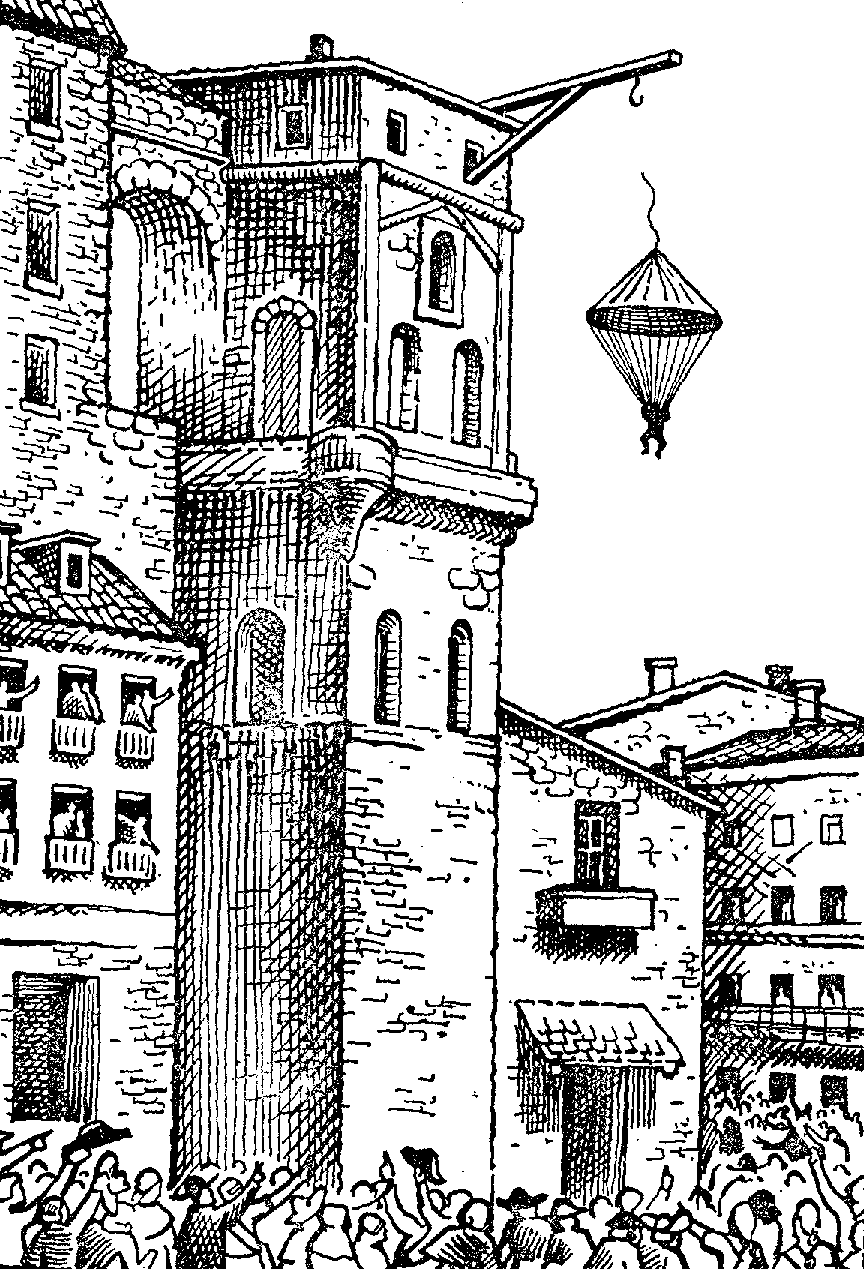
\includegraphics[height=8in] {images/01}}
    \caption{����� �.~��������� � ����� ������������ � ������ ��������
    � 1783 ����}\label{ris01}
\end{figure}

� 1731 ���� � ������ �������� ��������� ������ ���, �������� ��� ����� �
�������� �� ���. ��� ��� ������ ����� �������� � ��������� ������������.
� 1783 ���� �� ��������� ���� �������� ������ ����� � ����� ����������.
� ����� XVIII ���� ������ �� ��������� ����� ����������� �������
������������������. ����������� �� ���� ��� �����������, � ������ �� ���
����������� � ������������ ������ ��� �����. ��������� �������� �������������
�������� ����������, � ������� �������� ���������������� ���� �� � ������
������ ������������ ���������� �� �����.

���� ������������ �������� ����� ������ �������������. �� ����������� ������
�������� �������� ��������� �������� � ��� �������. � ������� 1783 ����
�.~�������� �������� � ������������� �� ��������������� ������ � �����
������������ � ������ �������� � ������������ ����������� (���.~\ref{ris01}).
�������������� ���� �������� \flqq�������\frqq, ������� ��������� ��
������������ ����� \flqq{}parachute\frqq, ��� ��������
\flqq{}parer\frqq~--- ������������� � \flqq{}chute\frqq~--- �������. ������
������������� ���������� ������� ��������� �� �����, ��� ��� ��� ����
�������� ����������� � ������� ���������� ����.

� 1785 ���� ���������������� �.~������� ������ �������, ������� �����������
���� ����� � ��������� ����� (���.~\ref{ris02}). ����� �������� ��������� ���� �
������������ ����� ��������� ���� � ��������. ��� ������ ���� ����������������
������ ��� ����������� ����� �� �������� ���� � �������������� ���������� ��
�����. ������ ����������� ������ ����������� �� ���� ������ ���� ��� �������.
� ����� �� ������������� ������� �� ������ ����� 1000 � ������� �������� ����,
� ��� ���� ������ ���������. ������� �������������� ����������������� ��
��������� � ������������ ��������� �� ����� ������ � ��������.

\begin{figure*}
    \centerline{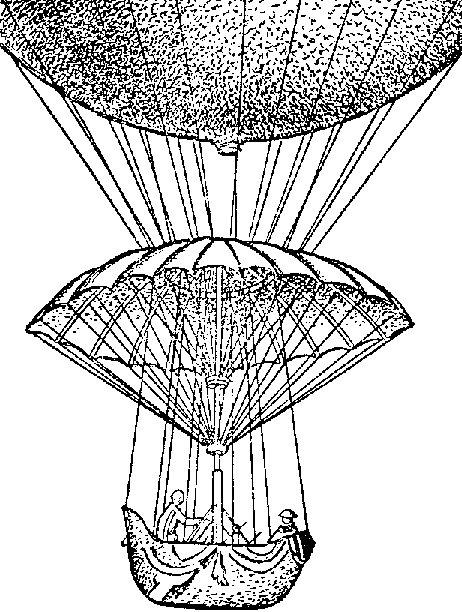
\includegraphics[height=3.3in] {images/02}}
    \caption{������ ����������� ������� ��������}\label{ris02}
\end{figure*}
\begin{figure*}
    \centerline{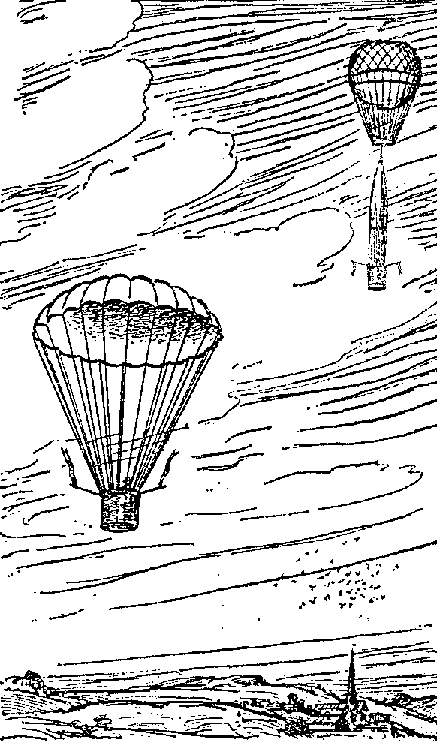
\includegraphics[height=3.3in] {images/03}}
    \caption{������������������� ������� ���������}\label{ris03}
\end{figure*}

������� ������������ ��� ������ ��� �������, �����������������
����������������� ����� ����������. �� �� ������ ��������� �� �����������
��������� �������� � ���������. ������� �� ���� �������� ������� � ��������
��������������� � ����� ����, � ������� ����������� �� �������� ��������.
� ������ ������ �������� �������������, � ������� � �����������������
���������� �� ����� � ������� ��������������� � ��� ��������. ����� ����
������ � ���������� � ��������� �������� �������� ��� ������ � ���������
(���.~\ref{ris03}). ��� ��� ������ ������������ ������ �������� � ����������
����.

����������� ��������� ���� ������� ���� ������� ������������ ������ ���
��������, ��� ��������� ��������� ��� �����������. �������� ��������� �������
� ������ ������ �������� �������� ���������, ����� ������� ������ ��������
�� ������ ����� �������. ��� ��������� � ������������ ���� �������������
������������ ������ � �� ��� ��� ����������� � ����������� ��������� �����
����.

����� ����������� ��������, �� ������������ ������������, ��������� � �����
������� ���������� �������. ��� ������� ���� ����� ������������ ������, ���,
�� ������ ������������, ������ ���� ������� ������������ ������ �� �����
��������. ������ ��� �������� ������� �� ���� ���� �������� �� ��������
����������� ��������. 27 �������� 1834 ���� �� �������� �� ��������� �
������ ������ � ��������� ����������������� ������. �� ������ 1000 � ����
��������� �������, ������� ����������� ������� ������ � ��� �������������.
������ 3--4 � ����� ��������� �������� �� ��������� ����� ��������
���������, �� ����� ������ �������� �� ��������, ��������, � �������
��������. ������� �����.

� ������ XIX ���� ���� ����������� ������� � �������� ����������� ���������.
�� ��� ������� ����������� ��� ���-���: �����, �������, �������, ����,
��������. �� ������� � ���� ������� � ��� ������ ���������� ����� �� ����.

� ����� XIX ���� ���������� ��������� ����� ���������-�� ���������� � �
�������� ��� �������� �������� ���������� ������. ������ � ��������� ���������
������������-�������������� �������� � ����������� �� � ����� ��������
����������� �������� ��� ������� ����������� ��������� ��� ������������������
����������� ���������, ��� ��� ������ ��������, ������� � ������, � ���
���������� ������� � ������������� ���� ���������.

����� ������������-��������� ���� ������� ������ ���� �������� �����
������������ ������������ ��������, ����, �������� ���������� �� ������
��������� ����������� � ����, �������� �������� ����������� � ��.

��������� ������� ������������ ������, ����������� �������� ����. � �������
�� ������ ���� �������� ������ � ��������� ��������� � ��������� ��������.
������ ������ ������ �� �������� ����������� �������, ������� ��������� �����
���������� ��������.

������ XX ���� �������������� ������ ��������� �������. ������ �� ���������
����������� �������� ��������. �� ������ � ������������� ����������� �
����������� ����-��� �� ���������� ������ ������ ���������� ��������� � �
������ ��������. ��������� ������ ������������� � ���������� �� ���������
������� ��������. ����� ��������� ��� ����� ������ �������.

�� �������� �������� ��� �������� �������� � ��������� ��������� �������
������ ������������. ������ ������������� ������������ �������� ���
����������� ������ ������. ����������������� �� � 1909 ���� ������� ���������
���� �� �������, ������� � ��������� ��������� ���������� ������ �������
�������. ����� �������� �������, ����� ������ ��� �������� ������ ��������
����, ������� ��� ��������� ��������� ����� ������� ���������� ������� ��
��������.

������� ������� ����������� �� ����� � ������� ���������� ����������
��������� �� ����������. �� ������� ���� ��������� ������������� ����������,
�� ��-�� ��������� ����������� ��������� ��� �� �������� ���������
�����������.

����������� ����������� ���������� �������� ��� �������������������
������������ ��������.

� 1910 ���� ����������� ����������� ����� ������ � ������� ���� �������,
������� ��� � ��������� � ��������� �����. � ��� �� ���� �����������
������������ ��� ��� ������� ���� �������. ��� ���������� ������ �� �������
�� ����������� ��������, ��������� �� �������� ����� �������� �����
(���.~\ref{ris04}). ����� �� ����� ������ � ���������, �����������������
�����, �������� ����������� ������ ����. ��� ��� ������ ������ � ��������
������� �����. ������� ����� ������������ � ����������� ������ � ���������
����� �������� � ���������� � �������� ��������.

������ �������� �������� �������� ��� ������� ��������� �� ���� ������.
�������� ���� �����������, ����������� �������� �� �������, � ��� ��
������������ ��������� ��������� �������� � �������� ������.

\begin{figure}
    \centerline{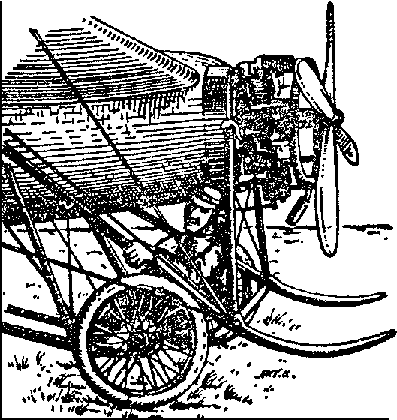
\includegraphics[height=2in] {images/04}}
    \caption{������������ ��� ����� �������}\label{ris04}
\end{figure}

� ������ �� ������������������ ������������� �������� ��� �������� ������
������������-�������� ���� ���������� �����������. � ������ �� �����
��������. ����� ������ � 1910 ����, �� ��� � 1911 ���� ��������������� ����
������ �����������~--- ����� ��� �������� ���������� ��������
(���.~\ref{ris05}). ���� ������������ ����������� � ���, ��� ����� ��������
����������� � ����������� ������������� �����, ������� ������� ������ ���
������ ��������� �������. �� ��� ����� ��� ��������� ������� � ��������
������� �������, �������, ����� ���� ��� ��������� �������� �������� ������,
����������� ����� � ��������� �����. ������������ �.\,�.~����������� �������
����� ������� ������, �� ��� ����� ��������� ���� ��� ������� � ��� �����.
�������, ��������� � �����, ��� ���� ������ � �������� ����� ��������� ��
�������� � ����� ������ �� ������� �������. �������������� ����� �����
������������� ��������, ������������ �������������, ����������� �� ��� ���.

\begin{figure}[b]
    \centerline{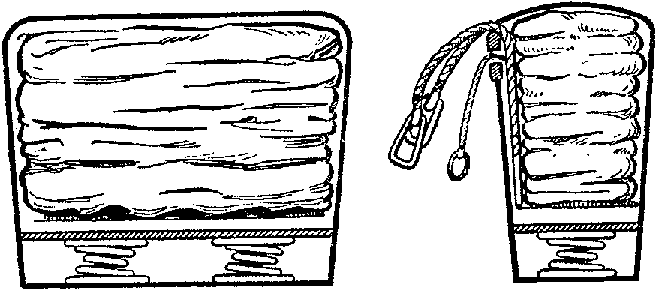
\includegraphics[height=1.6in] {images/05}}
    \caption{����� ������������ ��� �������� ���������� ��������}\label{ris05}
\end{figure}

������ �������� ������������� � �� ����� ������� ������������ �� �����.
��������� �� �������� ��������� �� ������ ���������� ����������� ��������
�������� � ������� ���������. ������������� ��������, ��� ��� ���������
�������� \flqq����� ���������� ���� � ����\frqq, � ������� ����� ������������
����������� �������� �������, �� ������� � ��������� ��� � �����������.

������ � ��������� �������� � ������� ���� ������ ������� �����, � ������
������� �������� ������� ��������������� ��������� ���������, �������������
��� ������������� ��������������� ����. ����������� �� ������ 200-300 �
�������� ��� ������� ������� ��� ��������� ����������. ���� ������� ������
� ��������-������������, ������������ ���� ��������� �������� �� ����������.
��� ���� ���� ������������ ��������� � ��������� ���������� ��������
������������, � ����� ����������� �� ������� �������� \flqq������\frqq.
� ������ ����� � ������� ��������� �������� ����� 50 �������
��������-������������.

\section{�������� ����������� � ����}

����� ������� ����������� ���������������� ��������� � ����� ������ ������ ��
����������� ������� ������� ������������� ���������� ���� ����� �� ����������
� �������. ������ ������ ��� �������� � ��� ������ ���� ����������. ������ ��
����� ����� �������������� ��� ������������ ������������� ���������.

� ���������� �� ������� ������ ������� ���������� ������� ���������
��������� �������� ��������� ������������, \flqq������\frqq{} �
\flqq��������\frqq, ������� ���������� � ����������� �������.

�������� ��������� ����������� ������ ���������� � ����������� ������������
������� ������� ������� �������� ������ ����������� �����������, �����������
������������ ������ � ���������. ����� �� ������ � ��������� ������ ������ �
��������� �������� ������������ 18-�� ���������� �������������������� ������
�.\,�.~����������. ���� ������������� ������ ��� �������� � ���������
�������� ������� �����~--- 23 ������� 1919 ���� � �������� ������. � 1921 ����
������ ���������� � ������� � ���������� ��������� ��������� �������������
������������������� �����, �� ��-�� ������ �������� ��������� ������ ��������
����������: ��� ����� �� ������� �����������, �� �������� ������������
��������, ������ ������� �������� \flqq������\frqq.

� 1926 ���� ��������� ������������� �������� �� ������� �������� ���������
�����, � ������-������������� �������� ���������� ����� ������ ��
������������� ���������. ������������ ���� ������ ������������� ��������
\flqq�����\frqq. ���� ������� ������������ �� �������, � ������ ������ ���
�������� ��� �������, ��� ��������� � �������� ����� �������� ����� ���������
��������, ��� �������� ������� �� ���� ��������� � �� ����� �����, ����
��������� �������, ������������������ ������ ������������� � ��� �����
��������� �������� � ����� ��������� �������� ��� ���������.

������������ � ���� �.\,�.~������������ ���� ������������� �����������
���������� ����� �� ����������������� ������������ �� ����� ������ ���������
��-2 � ��-3.

������� � 1927 ����, ������� ���� � ����� ������ ������������ ���������������
��� ������� �� ������ ���������.

� ���� 1927 ���� ��������� ������ ������ �������� ���������� ������� ���
������ ��������. ������ ������-�������������� ��������� ���������� �����
�.\,�.~������, ���� ����� ���������� �����, �������-��������� ������� �
��������, �������� ��� �������� �������, ������������� ��������� � ������
��� ������������� ������.

������ ����������� ������ ��� ��������� ��������� ��������� ���\-����-������\-����
�.~���������, ���������� �������, �� �������� �� �������, � �.~��������,
������� ��������� �� ���������� ������������ � ������� ��������.

��� ��� ������ ������������ �������� ���� ������� ������� � ������������� �
���������� �������� ��� ������������� �������� �������� ��� ������ ��������.

� ������-��������� ����� ������ ���� ������� �����, �� �������������� �����
������ ��� �������� ������� ������� ������� ���������� ��������. �����������
���������� ������ ���� �������� ���������� �.\,�.~������. � 1929 ���� ��
������� � �������, ����� ������������ � ����������� ���������-������������
������. ��� �� �������� ��������� ������� � ���������. ������������� ��
������, ����� ��������� ����������� ������ ������� ������� � ��������� �
����������� ������ ������.

� ���� �� ���� ���� ������������ ��������������� ����, ������� ����������
�.~�������� � �.~����������. � ������ �� �������� ��������� � ���������
���������� ������� ������� ������� ������� ����������� ������������ �.~�������,
�.~������, �.~�������, �.~������, �.~����� � ������. ������� ������
������������� ������� ���������� ��������� �.~�������, �.~������, �.~�������,
�.~������, �.~���������, �.~������� � �.~������.

�� �������� ����� � ������ ���� ������� ��������� ������� �������������
���������, ����������� ������ �������� �������� �������� ��������� ���
��������� ���������� � ������ �������� �������� ������� ����������
������������� ������� � ���������.

26 ���� 1930 ���� ������ ������� ������������ ��� ������������ �.\,�.~������
������� ��������� ������ � ������������� ��������. ���� ���� ������� �������
������� ��������� �������� ����������� � ��������� �����.

���� ���������� ������� � ���������, ����������� �������� ���������, ��������
������������ ������� ����� ������� ����� ��� �����~--- ��������-���������
������. ������ �� ���� �������� �������� 12 ������������ � \flqq���
�����\frqq{} �� ������� ��� ����������� �������� ������ 2 ������� 1930 ����.
� ��� ��� ��������� \flqq�������� ������\frqq ����� ���������� ���� �������
�������� � ������.

� 1931 ���� ��� ����������� ��� �������� ������ ���� �� ����������
������������ ����������� ����. ������� ������������� �����: �.~����������,
�.~�����������, �.~������, �.~��������, �.~������, �.~��������, �.~���������,
�.~�������. ��� ������ �������� ����� ����� ������������ ��� ��������-���������
������ � ������� �������� �������� ����������� ��������� � ���������
����������.

25 ������ 1931 ���� IX ����� ����� ������ ������� ��� ������-��������� ������.
� ������ ������ ����������� ���������. ������ � ��������� ����� �������� ��
������ �������, �� � ������� ����� ����������� ��������.

9 ���� 1931 ���� ������� � ���� ��������� ������ � ��������� �������~---
�.~��������.

����������� ���������� ������� � 1933 ���� ���� �������� �����������. ����
������� ������ ���������� �����, � ������� ��� ������������ �.~�����������
����� ���������� �������������� ����� ��� ���������� ������.

������ 1932--1935 ����� ���� �������� ������� ������ ���������� � �������
��������. 22 ��� 1932 ���� ������ �.~��������� ��������� ������ ������
��������� ������, ��������, �� ��������� ��������, 600 �, � 18 ������� ����
�� ���� ���������� ����������� ������ �.~������ �������� ������ ��������
������, ������� ������� �� ������ 5200 �.

29 �������� 1932 ���� ������ �.~��������� ������� ������ ���������� �
��������, �� ��������� ��������, 1600 �. ������ ����� ������ ����� ���������
����� ���������-���������� ������� �������. � �����, �� ���� ��������
�����������, ���� ����������� ��� ��� ���� ���� ���������, �������� �������
� ��������� ���������.

� ������� 1933 ���� �.~�������� �������� ���������� ���������� �������
�� 2200 �, � ������ ���� ������� �.~�������� ��������, �� ��������� ��������,
3170 �.

21 ������� 1933 ���� �.~��������� ���� ����� ����������� ������� � ��������
������. �� ��������, �� ��������� ��������, 6200 �. � � ������� 1933 ����
�.~������ ������� ��������� �� 7050 �.

16 ���� 1934 ���� �.~��������� ������ ���� ������ ����������� ����, ��������
� ��������� ������� 7900 �. ��� ���������� ���� ������ � ���� �� 1938 ����.

� 1934 ���� ������ �������� ������ ��������� � �������. 11 ������� 1934 ����
������������ �.~������� ��������� � ��������� ������� 2500 �, � 13 �������
������ ���������� �.~�������. ��� �� ���������� ��������, �������� �����
2700 �. ��� ���������� ���� ���������������� � �������� ������� ��������
������� ����� ������.

������� ���������� ������������ ���� �������� ��������� � 1934 ���� ���������
������ \flqq������ ����������� ������ ����\frqq. ������� ��� �����������
�.~�����, ����������� � ���� ������� 32 ������, �.~����������~-- 101,
�.~�������~-- 112, �.~��������~-- 113, �.~������~-- 106, �.~���������~-- 96,
�.~�������~-- 26, �.~������~-- 36, �.~�������~-- 81, �.~��������~-- 86,
�.~������~-- 87, �.~���������~-- 80, �.~�������~-- 100, �.~�����~-- 103.

�������� ������������ ������� � ����� ������� � ��������-��������� �����.
������ 1935 ���� �� ������� ��������� �������� ������ � \flqq��� �����\frqq{}
�������� 1200 ������������, ������� ������ �������� � ���������� ������� ���
������� ������� �� 2500 ������� � ������ ��������. � ���� �� ���� �� �������
������������ �������� ������ ������������ � \flqq��� �����\frqq{} 1800
������������ � ��� ������� ���������� ������ � ���������� 5700 ������� �
�������� � ������� �����������.

�������� �� I ���������� ��������� ����������� � 1935 ����, ������ �������,
������ ���������� ����� �.\,�.~��������� ������: \flqq \ldots ��\-��\-���\-���
����~--- ��� ���� �� �������� ������ � ���������� ������� ��������~--- �������
������� ������ � ������� �� ��� ����� ������, ���������� ��������, � ���
������ ������� ����� ������ ����\frqq.

� ����� 1935 ���� ��� ������ ����������� �������� ����, ������� ������������
������ ���� ����������-���������� �������������� ������. ����������� ��������
��� ������ � ����� ������������� ����������� ��������� (���) � ����
������������ ��������� ����������� ����� �� ������������� �����.

1935 ��� ��� ����������� ��� ����� ����� ������ �������� � ����� ����������
�����������~--- 4 ��� ���� ������������ ������������� ��� ���� � �����������
������� ������������ ������ �������� ���������� �����. ������� ������ ����
���������� �.~�����, �.~���������, �.~������, �.~�������, �.~��������,
�.~��������. ������ ������� ������ ���� ������� �.~�����������,
�.~������������, �.~��������, �.~��������, �.~������, �.~�������,
�.~����������, �.~��������, �.~��������, �.~���������.

������ �������� ���� ���� ���������� � ������ ������ ������������. �����
������ ��� ������ �.~���������, �.~����������, �.~������� � �.~�����������,
����� ������� ������~--- �.~����������, �.~���������, �.~���������, �.~�����.

������������� ������� ������ � ������������� ���� ����������� � 1935 ����
���������� ��� ��� ���������� ���������� � �������� �������. 8 ���� �.~������
�������� ������ � ������ 7445 �, 17 ���� ������ ������� � ������� �.~���������,
�.~��������, �.~����������, �.~����������, �.~�������� � �.~�����������
��������� ������ � ������ 7035 �. 23 ���� �.~�������� ������� � ��������� �
������ 7750 �, � 2 ������� �.~�������� � �.~��������� �������� ������� ��
������ 7923 �. ��� ���������� ������, ������� ����������� �������� ����������
���������� ������������. ������� ��������, ��� ��� ��� ������ ����������� ���
������������ �������. �� ���������� ��������� ���������� �.~�������� �
�.~��������� ���� ���������� ������� ������� ������.

� 1935 ���� ���������� ���������� �������������� ������ ����������� ���������
���������� �����������. 12 ���� ������������ ������ � ������������� ��������
����������� �������� ����, ��� ������������� � �����������
����������-���������� ������, ����������� ����������� �������� � ������������.

� ����� ����������� �� ������� �� ������������ ��� ���� ������ ���������� �����
�.\,�.~��������� ������������ ��������� �� ������� ����������� ������ ��
�������� ������-���������� ����� ������, ������� �������������� �������� �
��������� ���� ����� ������.

��������� ���������� ����������� ���� ������������ ������ ���������� ������
������������, ������� ��� �������� � 6 �� 15 ������� 1935 ���� � ������ ��
��������� ������.

����� ������� �� �������� ����������� � ������� � ��������� � ���������
�������� ��������� ����� ��������� ������-���������� ����������~--- ���������
����-������ � ������ ������ ��������� � ������������� ������ ��������, ����
�� ����� �������� �� �������, ������ ����� �� ������� � ������� � �������
����������� �����.

���� ���� ����������������� ���������� ������������ � ����� ������ ������ ��
������ ������ ��������� � ������� ������ ������������� �� ����������� ������.

� ���� ������ � ������� ���� ����������� ������������ ������� ������� 21
�������~--- ������������� ������ �������, �������� � ��������� ������. �����
� ������������� ����������� 148 �����������, ����� ������� ���� 20 ������.

������ ����� ������ ������� ������������ ��������� ���� � ������� �.~��������,
�.~���������, �.~������, �.~����������, �.~����������� � �.~��������.

� ��� ��� ���������� ������������ � ����� ������ ���������� ���������.

������ ���������� ������������, ����������� ����������� ��������� ��������
����������� ������, ���� ��������� � ���� 1940 ���� � ������ �� ���������
���������. � �� ��������� ������� �������������� � ��������� ������ ��
�������� �����������, ������ � ��������� � ��������� ��������, ����������
����-������ �� ������� � �������� �� �������������� ��������.

� ��������� ������ ������ � ���� ������-���������� ���������� ����������
�������� ������� �������.

1940 ��� ��� ����������� ���������� ������������� ������ �����������
������������. ���� �������� ������� �������� � �������� ������� ���� � �����.
������� ���������� ������� 24 ���� 1940 ���� �.~���������. �� �������� ������
� ������ 13\,025 � � ��������, �� ��������� �������� 11\,755 �. � ��� 1940
���� ������ �� 16 ������������ � ������� �.~��������, �.~������������,
�.~�����������, �.~���������, �.~�������, �.~��������, �.~���������,
�.~������, �.~���������, �.~������, �.~��������, �.~�����������,
�.~����������, �.~�������, �.~���������� � �.~������� ������� � ����
��������� ��������� �������� ������ � ������ 8400 �, ��������, �� ���������
��������, 7400 �.

������� ������������� ����� �������� ������� ���������� �������. �����������
������ ������ �� ���� ������� ������ �� ������ ���������. ������� �����������
� ���� ����� �����������-���������� �� ������� �.~��������, �.~���������,
�.~���������������. ������� ����� � ��� ���� ��������-��������� ������ ���
������������� �������� �.~��������� � ������ ������, �������������
����������-�����������.

�������, ���� ����������� ���������� ���������� � �������� �������������
�������� ����������� �.\,�.~��������, ����� ���� ������ �������� � ������� ��
����������� ������� ���������� �, ����� � ��������� ��� �� ������� �����������,
�������� ��������� �������� � ������������ � ���������.

� ������ ������� ������������� ����� ������� ���� ����� ������� ��������,
������� ������������ � ����� � ���������� ������� �����.

����� ����� ���������� � ����� ������ ����� ������ ��������� �������������.
��������� ����� �������� � ���������� ��������, ����� ����������� ��������.
����� ������������� ������ ������� ������ �� �������� ������� ��������� �
����� ������.

25 �������� 1945 ���� ���������� ��������� �.\,�.~������� �������� ������ �
������ 13\,108 �. �� �������� 12\,147 �, �� ��������� ��������, �� 167 �.

4 ������� 1947 ���� ��� �������� ������, ������������� �.~�������� � 1934 ����:
�.~������������ ��������� ������ � ��������� � ��������� �������� � ������
4500 �, �������� � ��������� ������� 71 �.

8 ������� 1947 ���� ���������� ��������� �.~������� �������� �������� ������ �
������ 12\,240 �. 13 ������� ����� �� ���� �.~������� ������ ������ ������ ��
13\,400 �.

���� ����������� ����� �������� � � ��������� �������. ������ � ������ 11\,200
� ��������� 31 ���� 1947 ���� ������ ������������ � ������� �.~��������,
�.~��������, �.~����������, �.~���������, �.~���������, �.~�������, �.~������
� �.~���������.

���������� ����������� � ��������� ������� ��� ������ �������� ������ ������
������ � ������� �.~��������, �.~������������, �.~��������� (�����������),
�.~�������������, �.~�������� (���������) � �.~����������, ����������� 29
�������� 1950 ���� � ������ 5600 �. ��� ��� ������ ������ ��������� ������
� ��������� � ��������� ��������. ������������ ������, �� ��������� ��������,
3533 �.

������ ���� ����������� �������� ������ 25\,485 � � ��������� �������
(�.~�������~-- 1 ������ 1962 ����) � ����� 16\,000 � � ��������� �������.

������ � �������, ����������� ��������� � �������� ������. ��� �����
������������� �������� ������ ������� ��������� ��������~--- �����������������.

������ ������ �������� ����������������� �������� 24 ���� 1947 ����
�.~���������. 13 ������ 1948 ���� �.~������� �������� ����������������� ��
�������� 764 ��/�.

���� ��� ������ � �������� ���� ��� ������ ������������� ���, � �������������
����������������� ������ ��������� ���������� �������-�����������. ������ ��
1957--1959 ������� ���� ����������������� �� ���������� ��������� � �������
����� ��������� ����� 60 ��������� ���������� ���. � ������������ ������
������ �� ������������� � ���������� ���������� � ����� ������ ��������� �
����� ���������� ��������, ��������� �������������� �.~���������,
�.~���������, �.~����������, �.~����������� � �������.

������� � 1953 ����, ����������� ���� ��������� �������� ����������� ����
������� ������������� ������������ �� ����������� ������. � 1954 ���� �
����-��� �� ������� �������� 2-� ��������� ���� �� ����������� ������.
� ���� ����������� ������������� ����������� ���� �� 1-� ���������� ��
�����������, � ��� ��� �� �����. �� 2-� ���������� ���� �����������
���������� ����������� ���� �����. ������ ����������� ��������� 31 ���������.
� ������� ���� ����� �.~��������, �.~��������, �.~�������, �.~������,
�.~������� � �.~������������. ������� �������� ������� ��� �.~����������,
��������~-- �.~����������.

� ��������� ������������ ������� ������ �� �������� ����������� � ������ 600 �,
��������������� ������ � ������ 1500 � � ������ � ��������� � ���������
�������� �� 20 � � ������ ����� �������.

������ ����������� �������� ���� �� ���� ������������� � ������� ������
�������� ��������� ��������� �.~��������. ���������� �������� ���� ����� ���
���������� �.~��������, ��������� ��� �.~�������.

�.~������������, ����������� ������� � ���������, ������ 8-� �����, � �����
������ ���� ������. � ��������� ������ �������� ����������� ����.

� ��� ��� ��������� ����������� ��������� �������� �������� ����� �� ����
����������� ���� � ������ ������������� �������������.

� 1975 ���� � ��������� � �.~��������� ��� �������� 1-� ��������� ������ ��
����������� ������, � ������� ������� ������� ������������� 17 �����.
�������� �� ���� �������������, ����������� ���� ������������������ �������
���������� ����������, �������� 23 ������� ������ �� 24-� �������������.
������ ���������� ��������� ������ ��������� ����������� ������� ������ ����
�.~������� � �.~������.

� 1978 ���� ����������� ���� ������� ������� � 14-� ���������� ���� ��
����������� ������, ����������� � ��������� � �.~�������.

���������� ��������� ���� ���� ������ ������ �������������� ������ ����� �����.
������� ������ ������ ������ ������������� �����.

����� �� ���� ���������� ���������� ������������� ��������� 7 �������,
13 ���������� � 8 ��������� �������.

������ � ����� ������ ��������� ���������� ���������� ������� ������� �����
������ � �������. �������� ���������� ����� 2000 ��������� ������������ ��
����������� ������, �� ������� ������������� ������ ��������, ������������ �
����������� ����� ����������� ���������� ������, ��������� �����������
���������� ������ ���������� ���������� �������������.

\chapter{������������ ����� ���������}

\section{���������-������������� ������� \mbox{�-1-5-�}}

���������-������������� ����������� ������� �-1-5-� ������������ ���
������������� ������� ���������� �����������-������������ � ���������
������������ ���������� � �������� ��������, ������� � ���� ����������
������� ���������� ��������.

������� ����������� � ���� ��������� ���������:\\
\mbox{\quad}� �������������� ���������� ����� � ����������� ����� � ������
�������� �����;\\
\mbox{\quad}� �������������� ���������� ����� � ����������� ����� � ������ �������
�������� ���������;\\
\mbox{\quad}� ������ ���������� �����.

� �������� �������� ������: ����� �� ��������, ��������� �������, ����� �
������� ��������, ����� ������, ������� �������� �������, ������������
��������������, �������� ���, ���������� �����. � �������� ����������� �������.

\begin{figure}[!htb]
    \begin{center}
    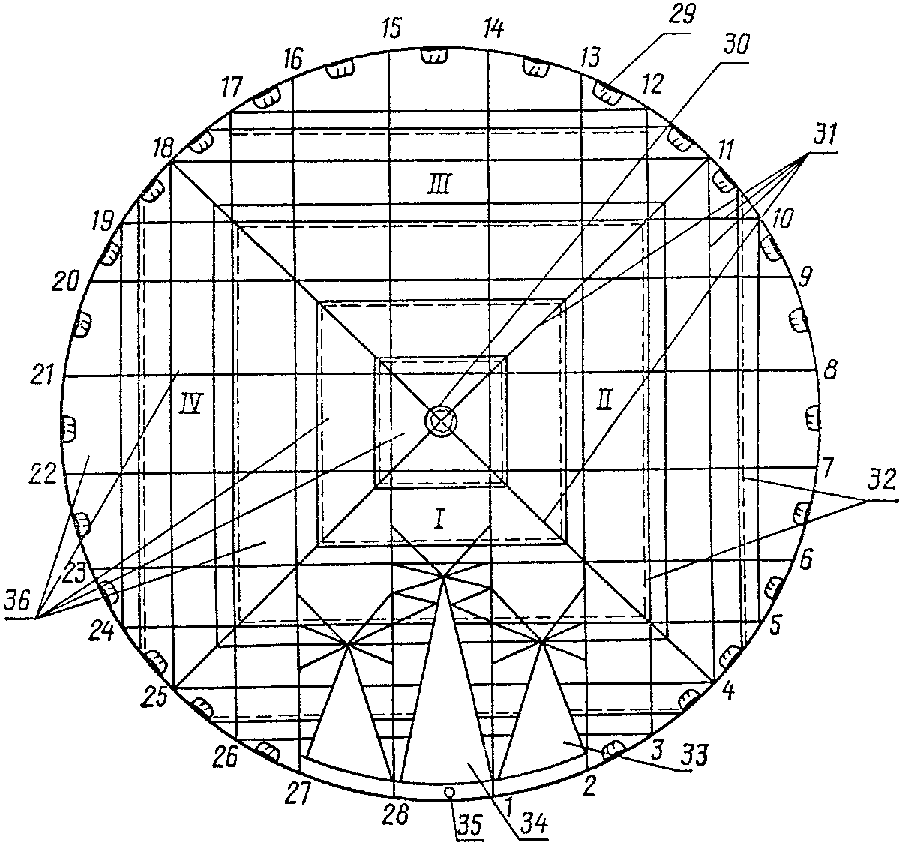
\includegraphics[width=320pt] {images/06}
    \caption{����� �������� �-1-5-�:}\label{ris06}
	{\scriptsize 1-28~--- ����� ��������� ����� � ������; 29~--- �������;
	30~--- �������� ���������; 31~--- ������������ ������; 32~--- ���
	��������; 33~--- ����� ����������� ���������; 34~--- �������
	����������� ���������; 35~--- ��������� ������; 36~--- ���������;
	I-II-III-IV~--- �������

	}
    \end{center}
\end{figure}

{\bf �����} �������� (���.~\ref{ris06}) ������� �����, �����������. �������
�� ������� ��������, ������ �� ������� ���� �� ���� ��������. ��� ��������
��������� �� ����������� ������ ����� ������������ ������ �� ����, ����������
�� ��������� 28 ������. � ������ ������ ������� �������� ���������, � �������
������������ �����, ����������� ��� ��������, �������� �������� �������.
����� ������� (����� 1 � 2-� 27 � 28-�, 28 � 1-�) ������ �������, ����������
���������� ������.

�� ���������� ����� ������� 1-� � 2-�, 28-� � 1-�, 27-� � 28-� ��������
����������� ���������. ��� ������ ������� �� ��� ��������� ���������� ����,
������������ ����� � �������������� �����������. ��������� ����� �������
1-� � 2-�, 27-� � 28-� �������� �������~--- ��� ������������� � ���
�������� � ���������� ��������, � ��������� ����� 1 � 28-� �������~--- � ���
���������� � ������ ��������. ����� ������ ����� ����� ��������� �������
�������������� �������� �� �����. 28 ����� ������ ������� �������� � ������,
������������� �� ��������� ������, � �������~--- � �����������, ������ �
��������� ����� ��������� �������. ����� ����� �������������� ���������������
��������. � 1-� � 28-� ������� �� ���������� 2 � �� ������-���������
����������� ������ ���������� � ����������, ��� ��������� ������� ���������
������� �����, � ����� ��������������� � �� ��� ������ �������. ������
���������� ��������� � ����������� ������, ������� �� ����� ��������� �������.
�����, ������ 82,5 �${}^2$.

\begin{figure}[!htb]
    \begin{center}
    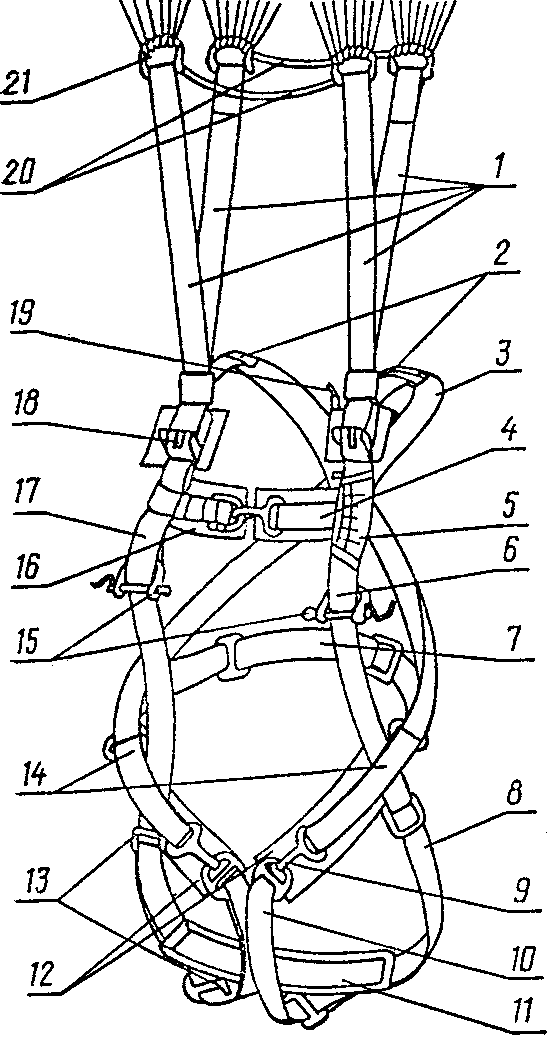
\includegraphics[height=3.5in] {images/07}
    \caption{��������� ������� �������� �-1-5-�:}\label{ris07}
	{\scriptsize 1~--- ��������� �����; 2~--- ������ ��������-�������� ��������;
	3~--- ��������-�������� �������; 4~--- ������� ��������� � ������� �
	���������; 5~--- ������ ��������� ������; 6~--- ����� �������� �����;
	7~--- ������� ������; 8~--- ������� �������� �����; 9~--- ��������;
	10~--- ������ �������; 11~--- �������� ��� �������� �������; 12~---
	�������������� ��� ��������� �����; 13~--- �������������� ������;
	14~--- �����-�����������; 15~--- ����� ��������� ��������� ��������;
	16~--- �������������� ������� ���������; 17~--- ������ �������� �����;
	18~--- ������������� ������; 19~--- ������ ��������� ������ ���������
	��������; 20~--- ��������� ���������� ��������� ������; 21~--- ���������
	������ ��� ������������� �����

	}
    \end{center}
\end{figure}

{\bf ��������� �������} (���.~\ref{ris07})~--- �������������� ����� �����
������� �� �������� � ������������. ��� ��������������� �� ���������� �����
� �������� � ���� ������� �������� ����� � �������� ���������� �������,
���������������� �������, ������� ������, ������� ��������� � ������ �������.
�� ������� �������� �����, �� ������ ����� �����������, ������������
�����-������ ��� ������������� ��������� ��������, � ���� ����� ������ ������
��� ������ ������� ��������� ��������. � ������ ����� �������� ����� ������
�������� ��� �������� ���������� ����������� ��� ��������.

��������� ������� ������������ �� ����� �������������� �������������� ��������
� �������� �� ����������� ��� ������ ��������� � �-�������� ������.

����� ��������� �-1-5-� �������� � ���������� ���������, ����������� �������
������� ���, ��������� �������� ������� ���� � �������
\flqq���������-������������� ������� ��-15 ����� 5\frqq.

\begin{figure}
    \begin{center}
	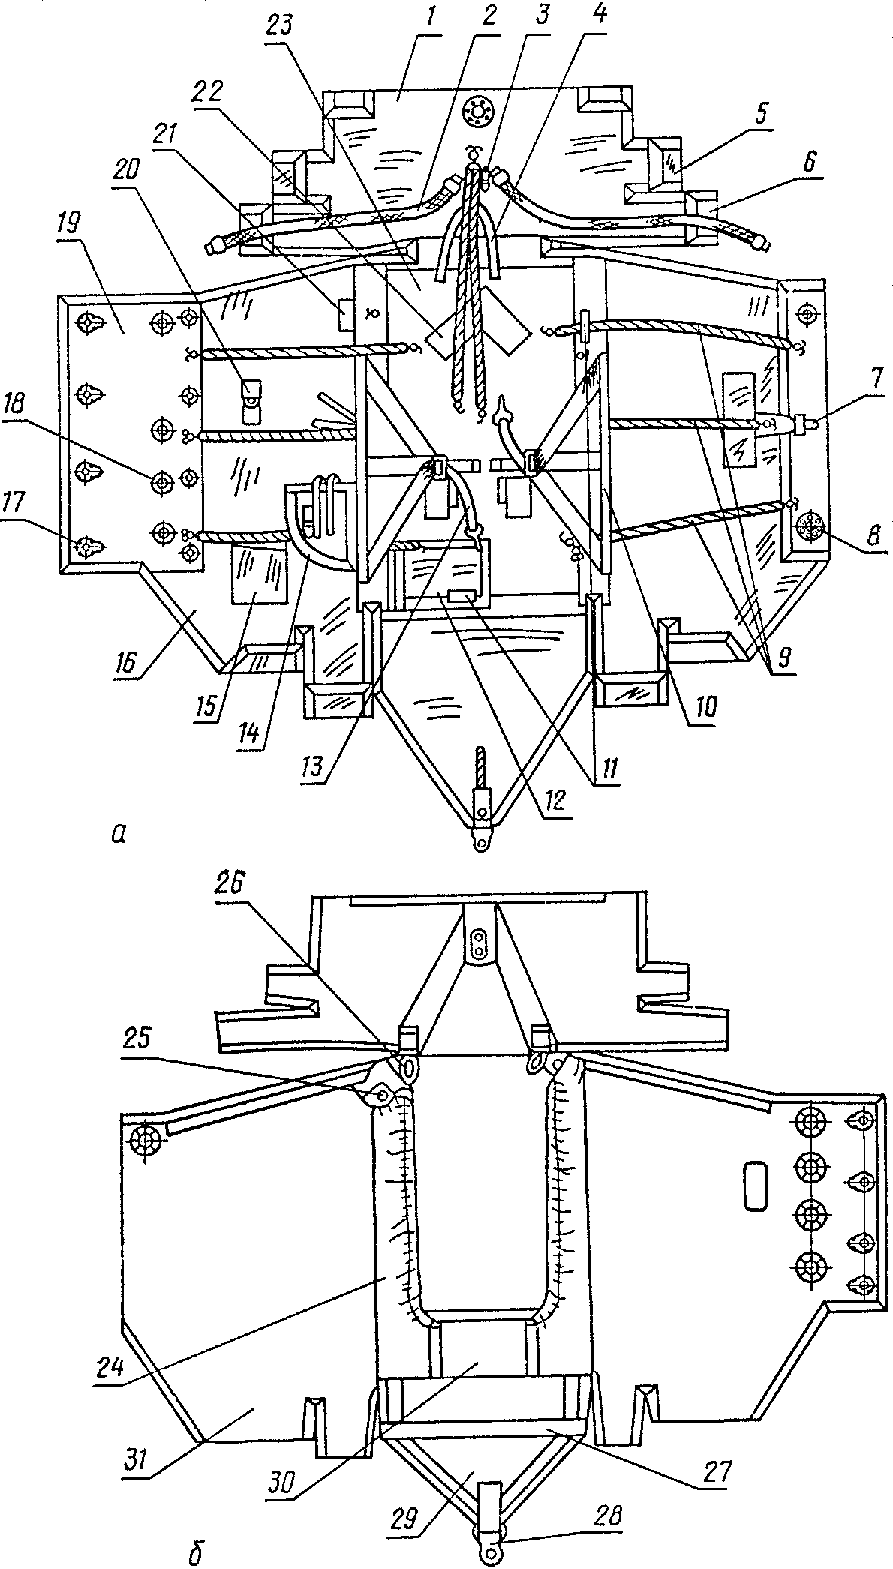
\includegraphics[height=6.7in] {images/08}
	\caption{����� �������� �-1-5-�:}\label{ris08}
	{\scriptsize �~--- ��� � ������� �������; �~--- ��� � ���������� �������;\\
	1~--- ������� ������; 2~--- ������ ������; 3~--- �������� ���������
	������� ���-�; 4~--- �����-�������; 5~--- ���� ��� ������ ���������
	������; 6~--- ��������-�������; 7~--- �������� ���������� ������;
	5~--- ������; 9~--- �������� ������; 10~--- ������� � �������;
	11~--- ������ �������� �����; 12~--- ������ ��� ��������; 13~---
	����� ��������� ��������� ��������; 14~--- ������ ��������� �������
	���-�; 15~--- ������ �������� ��������� ����; 16~--- ������ ������;
	17~--- ������-��������� ������������������ �������; 18~--- �������;
	19~--- ����������������� ������; 20~--- ������ ��� ���������
	��������� ����; 21~--- ����� ��������� ������; 22~--- ����� ���������
	����� � ��������� �������; 23~--- ��� �����; 24~--- ������� ��� �����;
	25~--- ���� ��������� �����; 26~--- ���� ��������� �����; 27~---
	�������� ���������; 28~--- ������-������; 29~--- ������ ������;
	30~--- ������, �������������� �������� ������ �� ��� �����;
	31~--- ����� ������

	}
    \end{center}
\end{figure}

{\bf �����} (���.~\ref{ris08}) ������������ ��� ������� � ���� ������ � �����,
�����, ����� ��������� ������ ��������� �������, � ��������� �������� ��������.
��� ������ ����������� ����� ����� �������� � ��������� �������.

����� ������� �� ��� � ������� ��������~--- ���� �������, �������� � �������.
� �������� ������� ������� ��� ������ ������, �������� � ���������� ����������
� �����-������� ��� ��������� ������������������� �������. � ���������
�������� ������� ������� ��� ���� ��� ������ ��������� ������ ���������
�������. ������� � ������� ������� ����� �������� ���������� � ���������,
������� ������������ ����� � ��������� � ���� ������� �� ����������� � ���
�������� �� ������ ������� ���������� �������� ��������������� �����. ���
��������� ����� � �������� ��������� �� �������� ������� �������, ������,
�������� ������ � ������-������, ������� ����� ������� ����� � ������� �
�������� ��������� �������� � ����� ���������� ��������� ����� �������������
��������������.

������� ��������� �������� ����� �������������� ������� ��������� ��������,
�������������� � �������� � ��� ����� ��� ������ ������� � ������ (�� �������
�������� �� �� ���, � �� ������� � ������~-- �� �����). �� ������� ������
�������� ������� ������ � ��������� ����������. ����� ��� ţ ���������
��������� � ������ ������ ����� �� ������ ��� �����. �� ������� ������� �
������� ������� ������ ��� ������� � ��������, � ������� �������� �������
�������� �������. �� ������ ������� ������� ����������� ������ ��� ����������
������������������� �������, �����-������� ��� ��� ���������, ������ ���
������� �������� ��������� ���� � �����-������ ��������� ������.

������ ������� ������ �������� �� ���� ������ � ������� ����� �����������������
������, ��������������� ��� ��������� ����������� ��������������.
����������������� ������ �������� � ��������� ��� ������ ������� ���
������-����������. ��� ����� �������. ������ ��� ������������ ���� ���������.
� ������� ������� ��� ����� ������ ����� ��� ��������� ����� � ���������
�������, ������ ��� ����������� �������� �����, ����� ��� �� ��������� �
������ ��� ��������. � ���������� ������� ��� ����� �� ������� � ������
�������� ��������� ������ ����� � ������ ������� � ������, ��������������
�������� �� ��� ����� ���������� � ����� ������ � ������ ��������� ����� �
�������������� ���������������� ����������� ����� � �������. �� ����������
�������� �������� �������� ����������� ��������������� ����.

� �������� ������� ����� ������� ����� ��������� � �������� ��������������
��������. � ��������� ������������ ��������� ����, ������� ���������� ������
�����. ���� �������� ������-������� � �����, �������������� � �������� �������
����� � ���� ���������. ���� � ����� ��������� ���� �� ������ �������� ��������.

{\bf ������ ������} (���) ������, ��� ������������� �� ���������� ����������
� ����������� �������� ����� ������������� ��������������: ����~--- ���
������� � ���������� ��������� �����, ������~--- ��� ���������������.
������ ����������� �� �������������� ������� ������, ����������
���������������� ������. ������ ����� ������� � ���������� ��������� ������
����� ������ � �������� ������� �����, ������~--- � ��������� ������� ���
�������� ��������� ������.

������ ����� ��������������� ��������� ����������� ������ ����� ������ �
�������� ������� �����. ������ ��� ����� � ��������� ��������� �������� ���
������ � �������������� ����������� ����� � ��������� ������ ������������
��� ������ �����, � ��� ������� ���������~--- � ������ �� ������ �������
�������. ����� ������� ������� ������ 515 ��.

\begin{figure}[!htb]
    \begin{center}
	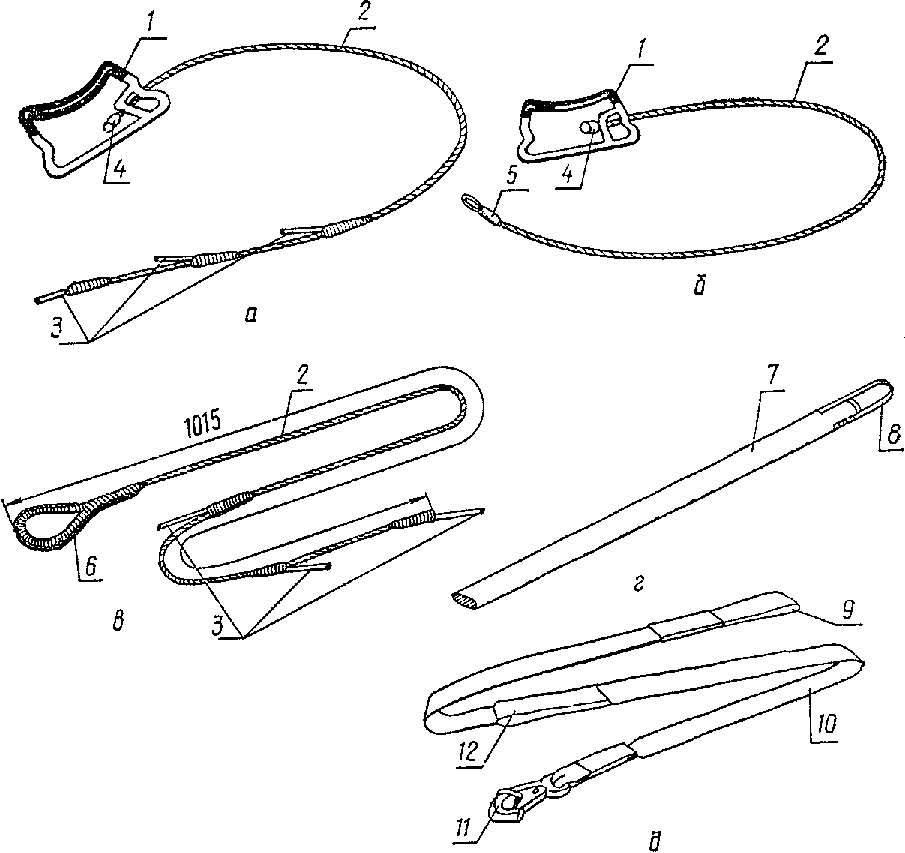
\includegraphics[height=4in] {images/09}
	\caption{������������ ��������������:}\label{ris09}
	{\scriptsize �~--- �������� ������; �~--- �������� ������ � ������ � ������;\\
	�~--- �������� ����; �~--- ����������������� �����; �~--- �������� ���;\\
	1~--- ������; 2~--- ����; 3~--- �������; 4~--- ������������;
	5~--- �����; 6~--- �������� �����; 7~--- ����������������� �����;
	8~--- ����� ���������� � �������� ������; 9~--- ����� �������������
	���� � ������� �����; 10~--- �������� ���; 11~--- �������;
	12~--- ����� ��� ������������� ����� ��������������� ���������

	}
    \end{center}
\end{figure}

{\bf ������������ ��������������} (���.~\ref{ris09}) �������� � ���� ��������
������ ������� ��������� � ������ � ����� ���������, �������� ������ � ������
� ������ ���������� ���������, ���� � ����� ��������� � ������ ��� ���������
���� ��������������� ��������� �����, ��� � ��������� ��� ���������������
��������� ����� ��� ��������� � ������ ������� ������������������� ���������
��������. �� ���� ��������������� ��������� �� ��������� ����������� �������
�������� ���������� ����������������� �����. �������� ��� ������. 3 �
���������� �� ����������� �����, �������������� �������� 1200 ���. �� �����
����� �� ����� ��������� ������� ��� ������������� � ����� ������ ��������,
� �� ������~--- ����� ��� ������������� ����� ��������������� ��������� ���
������� � �������������� ���������� ����� ��� ������������� ������� ������
��� ������� � �������������� ����������� �����. ��� ������� � ������
���������� �������� � ���� ����� �������� ��� ������ ������� ���������
����������� �������. �� ���������� 1,4 � ��� ����� ������ �����, ������������
����� ���������������� ��������� � ��������������� ��� ��������� ����� �����
� ����� ��������� ��� ���������� ������� � �������������� ����������� �����
� ��������� ������.

��� ������������� ���� �� ��������� (� ���������� ������ ����� � �����) ��
���� ������ ����� �� ���������������� �����. ��� ���������� �� ����� � ��
������� ����� ������ ������ � ���������.

\begin{figure}
    \begin{center}
	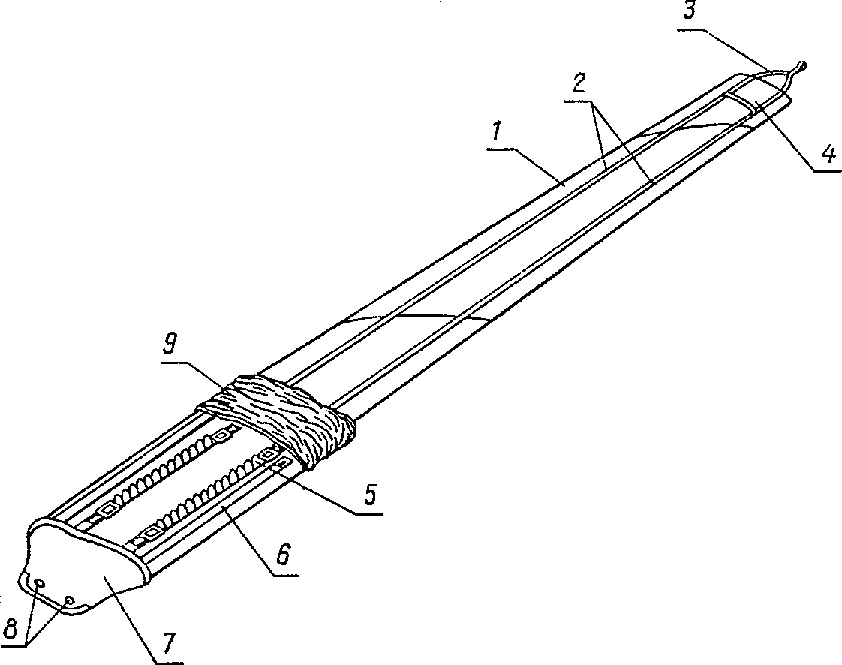
\includegraphics[height=3.3in] {images/10}
	\caption{����� ������ �������� �-1-5-�:}\label{ris10}
	{\scriptsize 1~--- ����� �����; 2~--- ������������ �����; 3~--- �������
	�����; 4~--- �������; 5~--- ��������� ����; 6~--- ����� ���
	���������� �����; 7~--- ������; 8~--- ���� ��� ���������� �������
	��� ��� ��������� �����; 9~--- �������������� �����

	}
    \end{center}
\end{figure}

{\bf �����} ������ (���.~\ref{ris10}) ������������ ��� ������������ ��������
���������� ������ � ������ � ���������� ������������ �������� �� ���� �
������ ���������. �� ����� ����� ������ � ���������� �� ��� ����� ������. ��
��������� ����� ������ �������, ������� � ������� ����� �������� ������� ���
������������� ��������� �������� �������� ��� ��������� ����.

� ������� ����� ����� ������ ��� �������, �������������� ������ ����� �� ���
� ���������� ����� � ������.

� ������ ����� ����� ����� ������, ���� ���� ������� ��������� ������� ���,
����������� ��� ��������� ��������� ��� � ��� ������������ ��������� �� ����,
� ������� ����������� ���������� ����, ��������� ����� ����������� ����� ���
������� �����.

������ ����� ������������� ��������������� ����� ��-����. �� ��� ������� ���
���������, � ������� ������������ ��������� ����. ��� ������� � ��� ����
����� ���������� ��������� �������. �� ��������� �����, � ��� ������ �����,
����� ��������������, ��������������� ���������� ����� ��� ������ ����� ��
�����.

{\bf ������� �������� �������} (���) ������������ ��� ���������� ����� �
��������� ������. �� ������� �� ������ �������� � ���������� ���������
(���.~\ref{ris11}).

������� ����� ������ �������� ����� ��������������� ����� � ���������, ��
����������� �������, � ������ �����, ���������� �� ��������� ��������� �
�������,~--- �� ���������� �����, ����� ����� ��������������� �����,
����������� � ����������.

\begin{figure}
    \begin{center}
	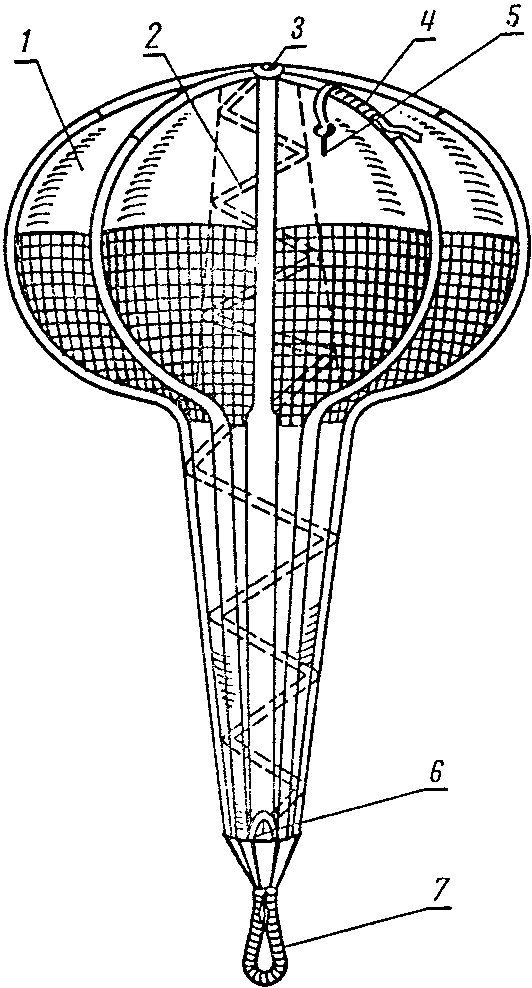
\includegraphics[height=3.5in] {images/11}
	\caption{������� �������� �������:}\label{ris11}
	{\scriptsize 1~--- ������ ��������; 2~--- ��������� ��������; 3~---
	������ � ��������� ������; 4~--- ������; 5~--- ����� �� ��������-�����;
	6~--- ����� ��� ��������� ���������� ���������; 7~--- ����

	}
    \end{center}
\end{figure}
\begin{figure}
    \begin{center}
	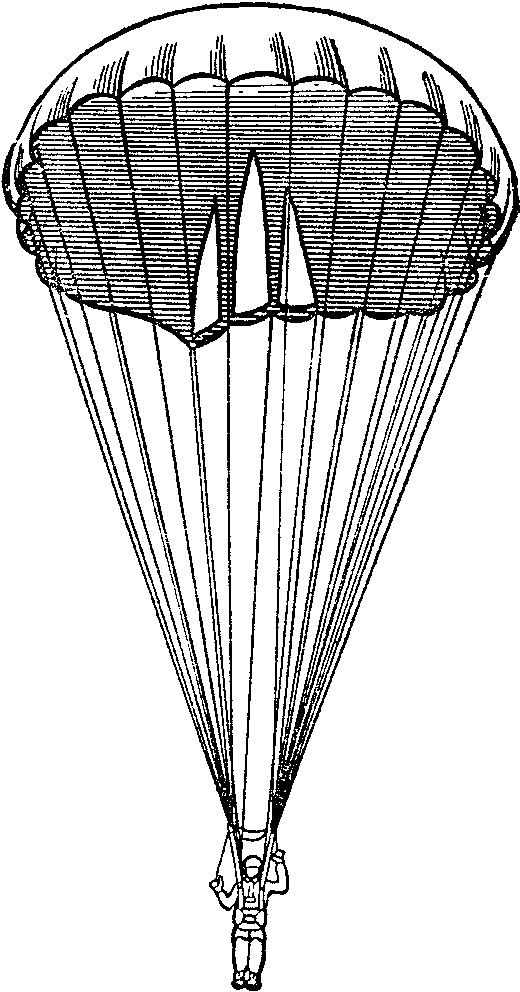
\includegraphics[height=3.5in] {images/12}
	\caption{�������� �������� �-1-5-� ������ ��� ��������� ������ ������
	����������}\label{ris12}
    \end{center}
\end{figure}

�� ������� ����������� ������ �������� ������ ������, ������������ �����,
���������� ������������� � �������������� �����������. � ����� �����������
���� ����, �� ������ ����������� �����, ���������� ������ � ��������� ������.

����� ����� ������� � ���� � �������� ������� ������. ��� ������ �����
�������� ������� �������� ������-������� � ������� ����� ������.

�� ����� �� ���� �� ������� ��������������� ����� ������� ������ � ����� ��
�������� ��� ��������� ���������� ��������� ��� � ��������� ����.

��������� �������� ������� �� ������ ������������� ������������� ������-����,
���������� ����������� ����� ���, � ���������� �������, �������������
������������ ������ ����������� � ���������� ������ ���.

�������-����� ������������ ���������, ������� ���������� � ������� � �������
������. ������� ����� ������� � ������� �� �������� ��������� ���, � �������
����� �������� ����� ����������� � ���������� ������� ���.

���������� ������� �������� ������������� �� ����������� �����, ����� ��������
��������� ��� ��������� � ��������� ��������� ����������� �����. �� ������
��������� ���������� ������� ��������� �������� � ������� ��� ���������
���������� ��������� � ������ ���������. ��� ��������� ����� ������������
����� ��������� ������� � ������� ����, ��������� ����� ������ ������ �
�������������� ��������-�����, ����������� �� ������ ��������.

��� ������� ��� � �����, ����� ��� �������, �������-���� ������������� ��
������ � ����������� �������. ��� ���� ��� ������������� ������������ �
������ � �������� � ���, �� �������� ����������� � ���������� �� ������ �����.

{\bf ���������� �����} ������������� ��� ������� � ��� �������� ���
��������������� � ��������. ��� ����� ������������� �����. � ������� ��
�������� ������� ��� ����� ��� ���������, ������ ��� �����, ����� � �����
��� ��������� �����.

����� ����������� �������� ��� ������ ���� ������-��������� � �����.

����� ������� �������� � ����� ������ �������� ������ ������, �����
������������ ������, ������� ������������ � ���������� � ����� ���
�������������.

{\bf ������� ��������} � ����������� �� ���������� ����� ��������� � �������
�� ��� ����� ��� � ��������� ����������� ���������. � ���� ��������� ������ �
����������� �������� �� ����������� ������������ � ����������, �������� ��
������� � �������, �������, �������� � ������. ��� ������ ������ ������� ���
�������, ��������� ��� ��������� ������. ����� \flqq����������� ��
������������\frqq{} ����������� ������� �����������.

{\it ������ ��������} �-1-5-� {\it � �������} ������� ��� ������� ����������
���� ���������� �� ��� ������������.

� ����������� �� ��������� ��������� ������� �-1-5-� ����� ��������� ��
�������:\\
\mbox{\quad}150--600 �~--- ������ � �������� ��������������� ������-��� �����;\\
\mbox{\quad}600 � � ����~--- � ������ ���������� �����.

�������� �������� ��� �������������� �������� �������� � �������� �� ������
��������� 180 ��/�, ��� ������ ���������~--- 250 ��/�.

������� �-1-5-� ��������� ��������� ������ � ��������� � ���������.
������������ ���������� � ������ ���������� ������ ��� ���� �� ��������� 10.

������� ������������ �������� �������� ��� ����� ����� ���������� �����������
�� ����� 120 �� �� ������� 30--35 � �� ����� ��� ����������� �����������
�������� �� ��������� 5�/�.

��� �������� �� ����������� ������ ���������, ������������� � ��� ������
��������, ������������ ����������� ������ � �������������� ��������� ��
��������� �� 2,5 �/�.

����� ��������������� ������ ������������ ��� ������ ��� ����� ����� ���������
����� ����������. ������� ���������� � ������� ��������� ��������� ������
���������� �� 12--14 �. �������� �������������� �� ���� ����������� �������
����� �������, ���������� �� ������������� ��������� (���.~\ref{ris12}).

\section{�������� ������� �-5}

�������� ������� ����������� ��� ����������� ����������� �����������
����������� ��� ���������� �� ������-������������� ������� � ������
����������� ��������� � ������ ������ ��������� ��������.

������� �-5 ������� �� ������ �� ��������, ������������� ��������� �������,
�����, ������������� �������������� � ���������� �����. ������ �������
����� ���� �������.

{\bf ����� ��������} (���.~\ref{ris13}) ������� �����, �������� 50 �${}^2$,
������� �� ������� ��������, ������ �� ������� ���� �� ���� ��������������
��������. � ������ ������ ������� �������� ���������, ������� � �������
������� ��������� ������� ���������, ��������������� ��������� ����������
������ �� ���������� � ������ ������ ������.

��� �������� ��������� �� ����������� ������ ����� ������������ ������,
���������� � ������ ������ 24 ����� ��� ��������� �����. ������ � �������
������ ������� ���������� ������ � ��� ��������. ����� ����� � ���������
��������� 6,3 �. � ������ ����� ������ �������� � �������-����������� ��
��������� ������ ������������� ��������� �������~--- �� ����� ����� �
������ ������-����������. ��������� ����� ����� ������������
��������������� ��������. �� ���������� 1,4 � �� ������ ������ ������ ��
������� �������� �����, ����������� �� ��������� ������� �� � ����. ��
������ ������ �� ��������� ������ ��� �������� (����� 12-� � 24-�) ������
����������� �����. ����� 24-� � 1-� �������� ������� ��������� ������ �
������� �������� � ����� ��� �������.

\begin{figure}
    \begin{center}
	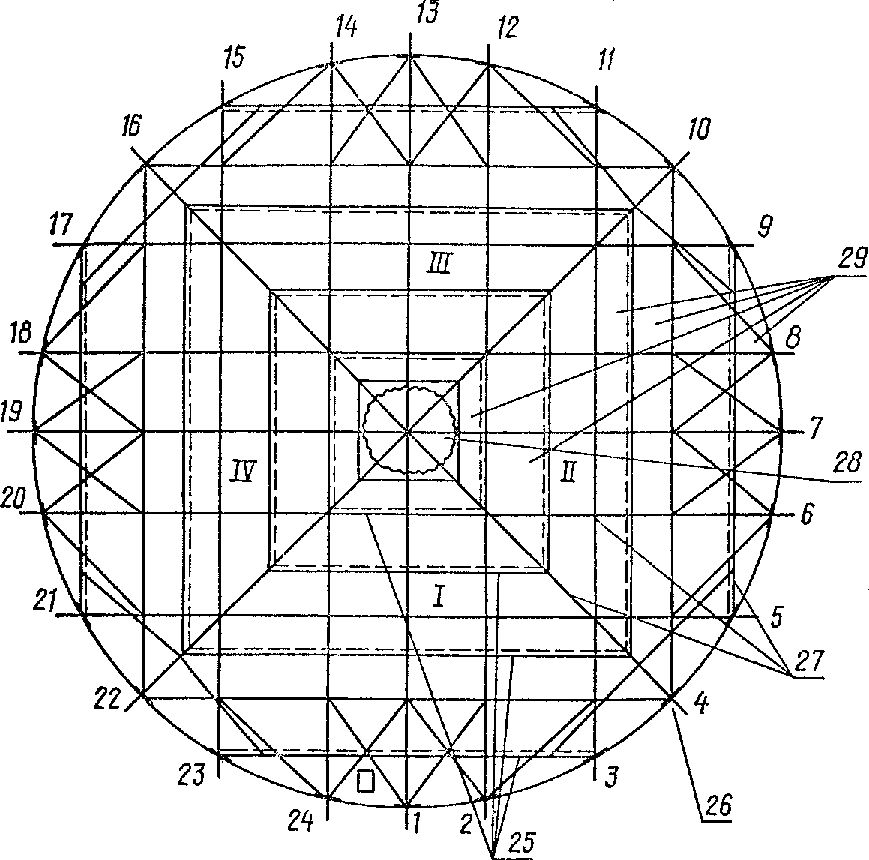
\includegraphics[height=4in] {images/13}
	\caption{����� �������� �-5:}\label{ris13}
	{\scriptsize 1~-- 24~--- ����� ��������� �����; 25~--- ��� ��������;
	26~--- ����������� �����; 27~--- ������������ ������; 28~---
	�������� ��������� � �������� �����������; 29~--- ��������� ������

	}
    \end{center}
\end{figure}
\begin{figure}
    \begin{center}
	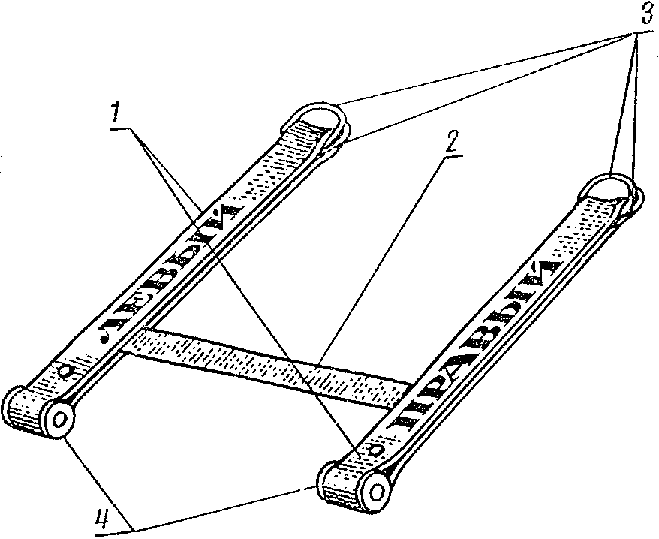
\includegraphics[height=2.7in] {images/14}
	\caption{������������� ��������� �������:}\label{ris14}
	{\scriptsize 1~--- ��������� �����; 2~--- ���������;
	3~--- ������-����������; 4~--- ������
	}
    \end{center}
\end{figure}

{\bf ������������� ��������� �������} (���.~\ref{ris14}) ������������� ���
���������� ������ ��������� �������� � ��������� �������� ��������� ��������.
��� ����������� �� ���������� ����� � ������� �� ���� �����, �����������
����� ����� ����������. ������ ����� ����� �� ��� ������-����������, �
������� �������� ������.

��� �������� ������������� ������������� ��������� ������� � ������ ���������
������� ��������� �������� � ����� ������������� ��������� ������� ���������
������. �� ������� ������� ����� �������� ������� \flqq�����\frqq{} �
\flqq ������\frqq. ������ ����� ����� ������ �������� ����� � ������������
������� �������� \flqq�-5\frqq. �� ����� ����� ��������� ��������� �����
��������.

{\bf ����� ��������} (���.~\ref{ris15}) ������������ ��� ������� � ����
������ �� �������� � ����� ��������� ������ ������������� ��������� �������.
�� ����� ���������������� ����� � ������� �������� ���������: �������,
������� �����, ������� ������ � ������. � �������� ������� ������� ������
��� ����, ��� ������ ��� ��������� �����, �������������� ������,
��������������� ��������� ����� ������ ��� ����-�� ��� ������� ����� � �����
��� ��������� ��������.

\begin{figure}
    \begin{center}
	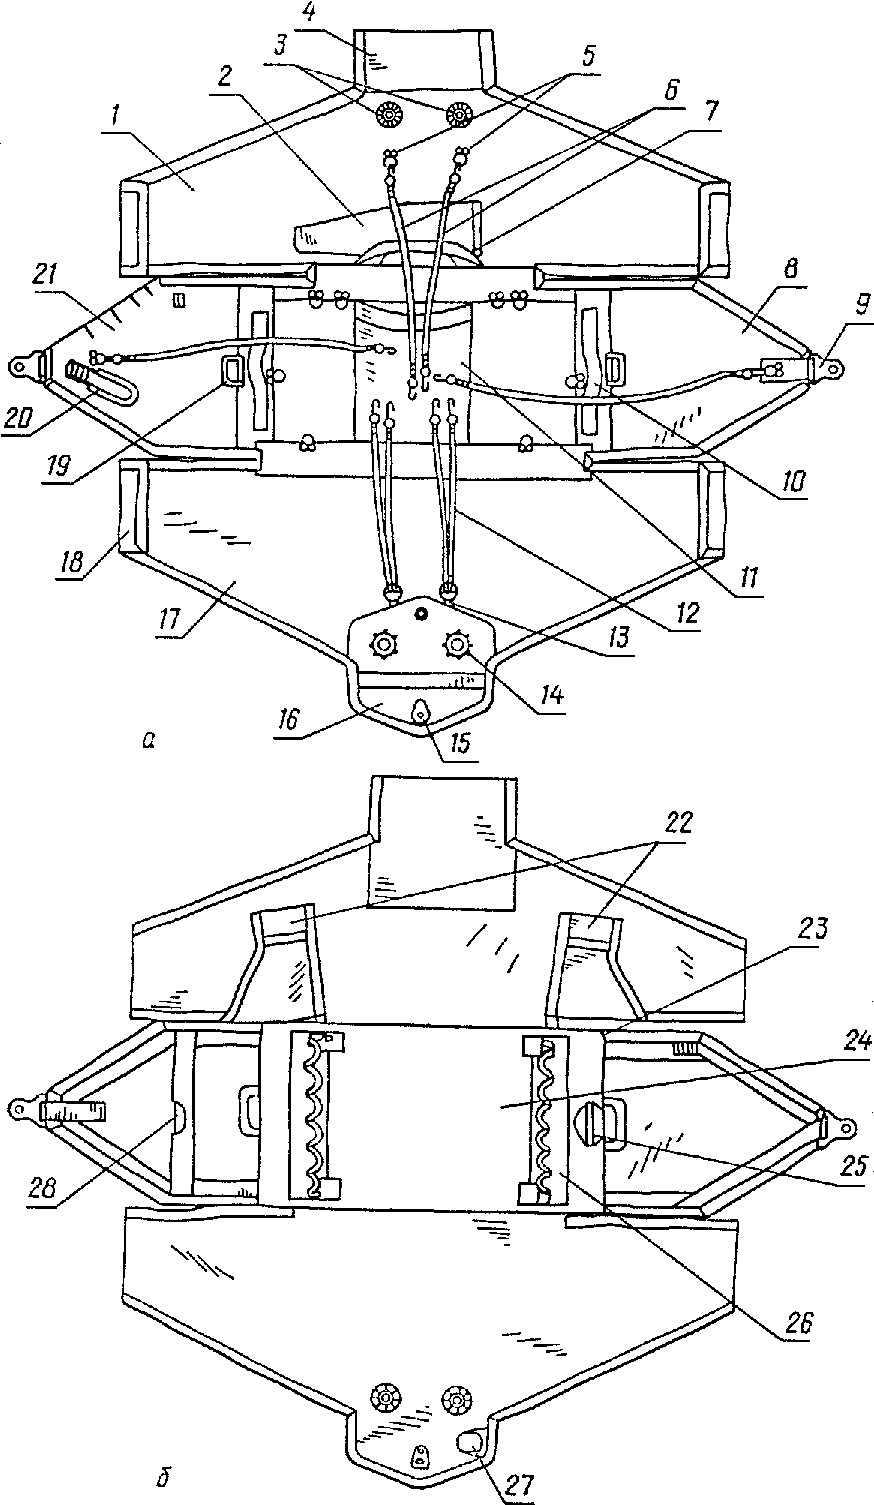
\includegraphics[height=6.8in] {images/15}
	\caption{����� �������� �-5:}\label{ris15}
	{\scriptsize �~--- ��� � ������� �������; �~--- ��� � ���������� �������;\\
	1~--- ������� ������; 2~--- ������ ��� ����; 3~--- ������;
	4~--- ����������������� ������; 5~--- ����� ��� ��������� ��������
	�����; 6~--- �������� ������; 7~--- ����� ��� ��������� ��������;
	8~--- ������� ������ ������; 9~--- ������-������; 10~--- �����
	��� ���������� ������ ������������ �������; 11~--- ������ ���
	��������; 12~--- ������� �������� ������; 13~--- ����� ���������
	������� �������� �����; 14~--- �������; 15~--- ������-��������;
	16~--- ����������������� ������; 17~--- ������ ������; 18~---
	������� ��� �������� ������� ��������; 19~--- ������; 20~---
	������ �����; 21~--- ������� ����� ������; 22~--- �������� ���
	�������� ��������; 23~--- ���� ��� ������ ��������� ������
	��������� �������; 24~--- ��� �����; 25~--- ���� ���������;
	26~--- ��������� ����; 27, 28~--- �������� ���������

	}
    \end{center}
\end{figure}

� ���������� ������� �������� ������� ����������� ��� ������� ��������,
�������������� ����� �� �����������. ����� ������� �������� � ���� �������
��� ��������� ��� ������ ������ ������������� ��������� ������� �� �����.

������� ����� ������ ����� ������-������, ������ ��������� ������, ������
�����, �������� ��� ��������� ���-�, ����� ��� ���������� ������
������������ ������� � ����� ��� ������������� �������� ������. ������
����� ������ 380 �� ������������ ����� �����, ������������� �� ��������
������������ ����� � ������� ���������� ��������. ���� ����� ������ ������
� �������� ��������� �������� ������� �������, ������ �������� �����
������������� ��������� ������� ��������� ������ � ������ � ������-�������.

������� ������ ������ ����� ������-������, ����� ��� ������������� ��������
������ � ����� ��� ������������� ������ ������������ �������. � ��� �������
������� ������������ �������� ���������. ������ ������ ����� ��� �����, �
������� �������������� �����-������, ��� ������� �������� ������, ���
�������, ����������������� ������, ���������� ������������ ������� �������,
������-�������� ��������� ������������������ ������� � �������� ��� ��������
�������� ��� ������� �����.

������� ����� ������ ������������ ������ ��������� ��������. ��� �����
������� � �������������� ������ ��� ����� ���������, � ����� ������� ���
��������� ����� � ��������� ������� ��������� ��������. �� ���������� �����
��� ����������� ����� ��� ��������� ��������� ��� ��� ������� � ��� �����.

����������� ��������������� �������� �-5 �� ��������������� �������������
�� ��� ����������� ������������ ���-�. ��� ������������� ��������� ��� ��
������� ��������� ���������� ��������� ���������, � ������: �� �������
������� ��� ����� �� ����� ������� � �������� ������ �������� ��������
����������� ���� ��������� ���-�, � �� ������ ������� �������~---
�����-������� (���.~\ref{ris16}). �� �������� 110 �� �� ������ ������-�������
�������� �������� � ���-������� ���������� ��� ������������� ������ ���-� �
�����-������� ��� ��� ���������.

\begin{figure}
    \begin{center}
	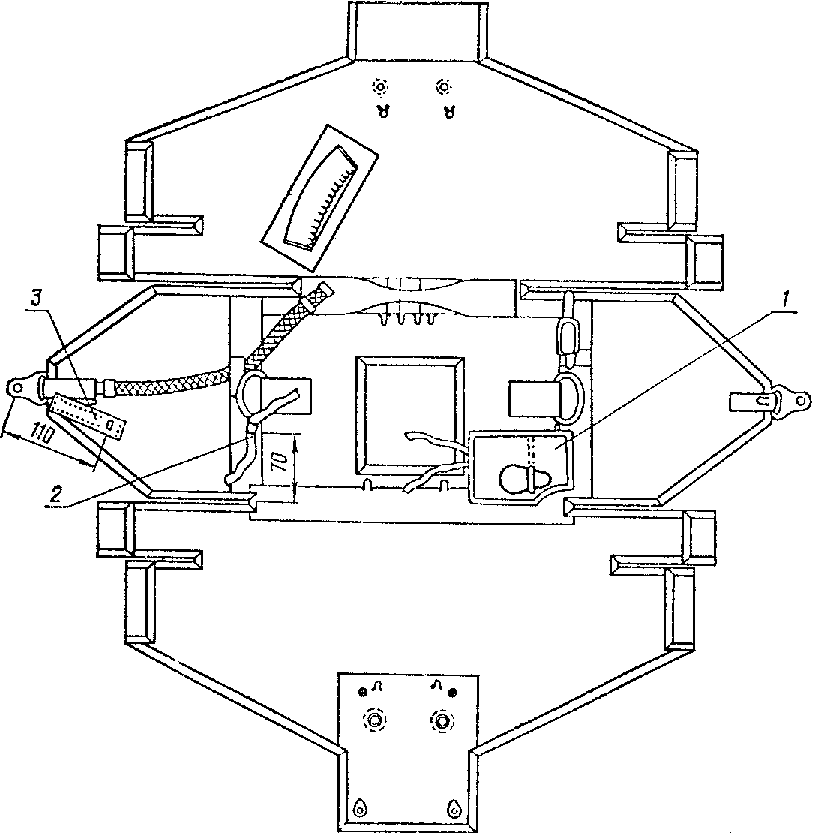
\includegraphics[height=3.5in] {images/16}
	\caption{��������� ����� �������� �-5 ��� ��������� ������� ���-�:}\label{ris16}
	{\scriptsize 1~--- ���� ��������� �������; 2~--- �����-�������;
	3~--- �������� ��������� �������

	}
    \end{center}
\end{figure}

�� ������ ������� � ����� ��������� ��������� �������� �������� ���������
������� �������� �������� ����, ������������� �� ����� ���-125 �������� �����
� ��� �������� � ������������� ��� ��������� ��������������� ��������.

���-� ��������� �� ������� ����� ��� ������ �������. ������ ��������� �������
������������� �� 350 � � ������ ���������������� �������� � ����� ����������
������� � ������������ �������. ������� � ������ ������������ �������������,
������������� �� ������� � �������� ���������, ������ ���� �� ����� 400 �.

������, ������������� �� �������� �������� ��� ������ ���� ��������� �
����������� ������, ���������. ��� ���� ��������� ������ � ����� �������������
������ ������� ���������� �������� ����� (����������� �� ��������� �-4 �
�-1-5-� ��� ��������� ������� ������� ����������� �������������� ������),
�� ������� ���������� ����� ������� � ����������� ����������� ������
(���.~\ref{ris17}).

\begin{figure}[!hbt]
    \begin{center}
	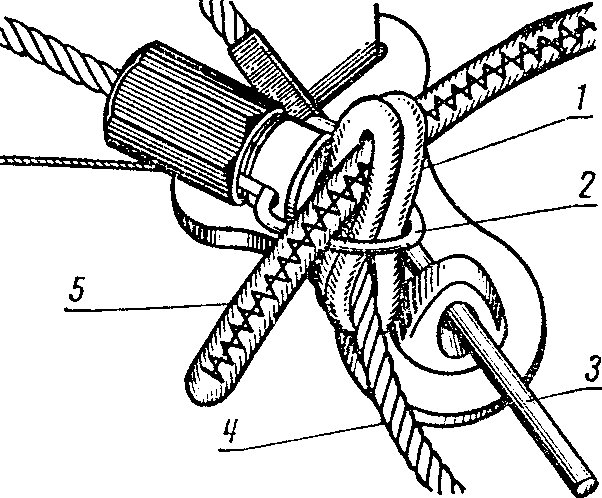
\includegraphics[height=2in] {images/17}
	\caption{������ ����� ������� ���-� �� ����� ��������� ������ �������� �-5}\label{ris17}
	{\scriptsize 1~--- �������� �����; 2~--- ����� ������� ���-�;
	3~--- ������ ������� ����� ��������� ������; 4~--- ����, ������
	� ������ ������� ��������� ������; 5~--- ������������� ����

	}
    \end{center}
\end{figure}

������ ��������� �������� �������� ������� ����� ������������ ���� � ������
�������� ��� ���������� ��������� ������ 600 �. ����� ��������� �������
���������� ��������� ������������ � �������� ��� ������ �� ����� ����� ���
��������� �� ��������.

������������ ��������� � �������� ����� �������� � ��� ����������������
������������ � ������� ��������� ���������� � ������ ������.

{\bf ������������ ��������������} ������������� ��� ��������� � ���������
����� ��������. ��� ������� �� ����� � ����� ���������, ������������,
��������� ��������� ������ �������������� �����. �� ������ ������� ���
�������, ������������ ��� � ������� �� �����. ��� �������� ������� �����
����� ������, �� ��������� � ���������, �������� �� 60${}^\circ$ � ��������.

{\bf ���������� �����} ������ ��� ������� � ��� �������� ��� ���������������
� ��������. ��� ����� ������������� ����� � ����������� �������,
��������������� � ���� ������ �� ���� ������-����������. ��� ��������
���������. ����� �������� ����� �������. ����� �� ��� ����� ������ ���
�������� �����.

������� �������� ������������ ��� ������� ���� ������ � ��������: �� ���
���������, ����� ������ ��� ��������, ����� ������������ ������ � ��.

{\it ������ �������� �-5 � �������.} ��� �������� � �������� �������������
�������������� ��� ������� ����� ������� �� ������� ����� � ����������� ���
�������, ������� ��� ��������� �������� ����� ������������ � �������.
�������� ����������, ��������� �� ��������, ������������� ������ ���������
��������� ������, ������� � ����� �������, ���������� �����, ��������� ��� �
����������� ����� � ���������� ������ �� ��� �����. ��� ������ ���������
������� ����� �����������, � �������� ���������� �� ��������� ������.

� ������, ���� ���������� �� ��������� �������� �� ���� � �������� ��������
������� ������ ��������, �� ����� �������� ���������� �� �������� ������
�������� ���-�.

��� ���������� ��������� �������� ������ ������������� �� ����� ���������
�������� ������ ���-� �������������� � ����������� ���������.

������� �-5 ����������� �� ������� �� ���� 100 � � ��� ��������� ������,
�� 120 �� 350 ��/�. ������� ������������ �������� �������� �� �������
30--35 � �� ����� ��� ����� ����� ���������� ����������� �� 120 �� ��
��������� 7,5 �/�.

��� ������� � ����������, �������� ���������� ����� ������������
(���� �-1-8), ������� �-5 ��������� ������.

\section{���������-������������� ������� ��-15 ����� 5}

����������� ���������-������������� ������� ��-15 ����� 5 ������������ ���
������� �����������-������������, ������� ���� � ���������� ������� �
���������� ����� �-1-5-� � �-4-4. ������� ������� �������� ������ ��� ������
�������� ��������� ���� ����������� � ������ ���������, ������� � ������� �
���� ��������� ����������� ����������, ������ ��������� ����� ����� �
��������� �������.

������� ��-15 ����� 5 ����� ������ ���� ������� ����������~--- ������
���������. � ��� �������� ������: ����� �� ��������, ����� �����, ���������
������� � ������� ���, ����� � ������ �������, ������������ ��������������,
����� ������, �������� ��������, �������������� �����, ����� ��� �������� �
���������������. ������ ������� ����� ���� �������, � ������� ��������� ���
�������� � ��� ����������� ��������� � ������������.

\begin{figure}
    \begin{center}
	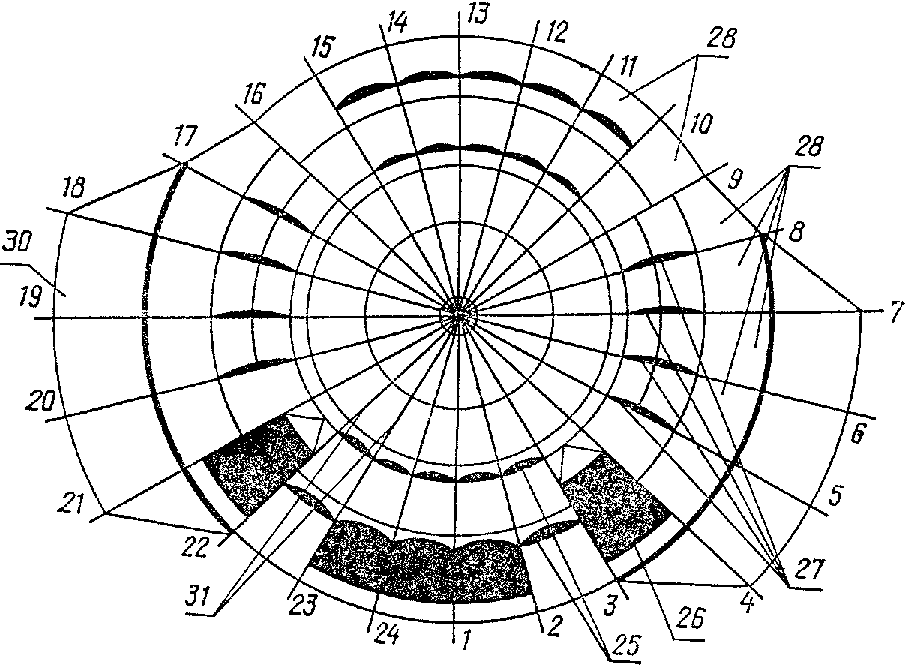
\includegraphics[height=3in] {images/18}
	\caption{����� �������� ��-15 ����� 5:}\label{ris18}
	{\scriptsize 1--24~--- ���������� ��� � ������� ��������; 25~--- �����;
	26~--- ��������� �������������� �����; 27~--- ���������� ����;
	28~--- �������; 29~--- ���������; 30~--- ������ ������;
	31~--- ���������� ���������

	}
    \end{center}
\end{figure}

����� �� �������� (���.~\ref{ris18}) ������������ ��� ����������� �����������
����������� � �������� �����. � ����� �� ����� ����� �����, ���������������
�� �������, ������� �� 16 �������� � 8 ��������, �������, � ���� �������,
������� �� �������. ������� ��� ��������� �������� ���������� ����. ��
�������� ����� �������� 21-� � 22-�, 3-� � 4-� ������� ���������
�������������� �����, � ����� �������� 22-� � 23-�, 23-� � 24-�, 24-� �
1-�, 1-� � 2-�, 2-� � 3-�, 10-� � 11-�, 11-� � 12-�, 12-� � 13-�, 13-� �
14-�, 14-� � 15-�~--- �����.

� �������� ����� ������ ����������� ���������� ��������� ��� ������ ��������
��� ��������� ��������. � �������� ����� ������ ����� �������� 17-� � 18-�
�������� ���������� ������� � ������� ���������������������. �� ����
�������������� ������� ������, ����������� ����� ������������� ������,
� ������� ������������ ��� ������ ����������.

�� ���������� ��� ������ � ������� ������� ���������� �������������� ������,
� ������� �������� �������������� �����.

�������� ��������� � ������ ������ ������ � ���� ������ ������� ����������
������.

� ������ ������ ������ ������� 24 ������. ������ ����� ����� �������� �
�������-����������� ��������� �������. ������ 1, 2, 3, 22, 23 � 24-� �����
���������� ���������. � ������ ������-���������� �� �������� ��������� ������
����������� �� ���� �����, � �� ������~--- �� ����.

� �������� ����� ������ ������� ������, �������, ����������� � ��������
���������, �������� �������� �������.

�� ������ ������ ������, ����� �� �����, ������� �� ���������� ������. ����
����� ������� ������ ������� �������. ����� �� ����� �������������� ����� ��
������-��������� ��������� �������~--- 9330 ��. ����� ����������� ������ ��
����� �������� ����� �� ������-��������� ��������� �������~--- 6200 ��. �����
����� ���������� �� ����� �� ��������� ����� 5000 ��.

������ �� ���� ����� ���������� ����������� �� ����� �� ������ ���������
������ ��������� ������� � ��� �������� �� ������������ �������������
���������, ���������� � ������� ����.

��� ����������� ���������� ������� �������� �� ���������� ������ ��������
�����:\\
\mbox{\quad}�� ������ ����� � ���� ������ �� �������� ����� �������� 6-� � 7-�,
18-� � 19-� � ������ ������ ������ � ���������� �������~--- ��� ������� �����
����������. �� ��� ����� ���������� ������ ����� ���������� ��� ������� ������;\\
\mbox{\quad}�� ���� ������� ������ �� ���������� 4100 �� �� ������-���������
��������� ������ ��������� �������, ���������� ������ ������� ����� � ����
�����, � �� ���������� 1300 ��, ���������� ����� �������.

� ������� ������ ������������ ����������� ������ �� ����� ���������� ���������;
������ ����� ������ ����������� � �������-����������� �������� ���������
������ ��������� �������.

\begin{figure}
    \begin{center}
	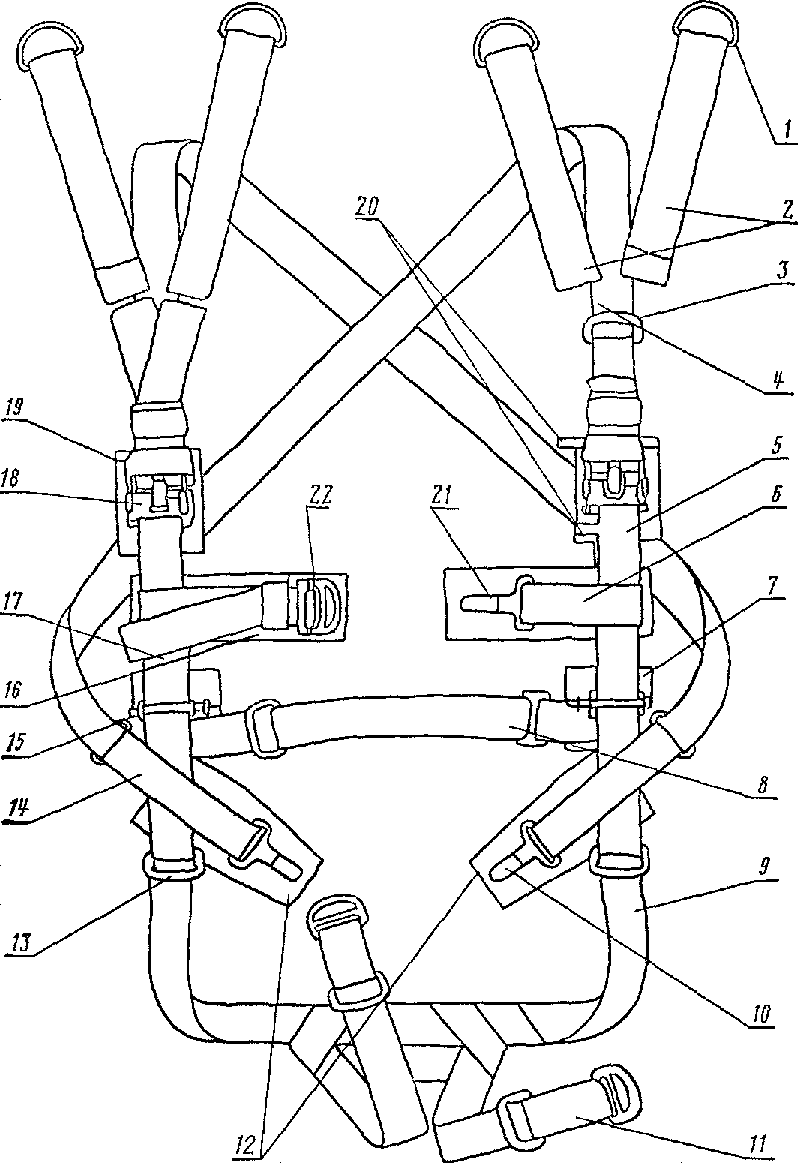
\includegraphics[height=5.8in] {images/19}
	\caption{��������� ������� �������� ��-15:}\label{ris19}
	{\scriptsize 1~--- ������-����������; 2~--- ��������� �����; 3~---
	������; 4~--- ��������-�������� �������; 5~--- ����� �������� �����;
	6~--- ����� ������� ���������; 7~--- �������������� ��� �����;
	8~--- ������� ������; 9~--- �������� �����; 10~---  �������;
	11~--- ������ ������; 12~--- ��������������; 13~--- ������;
	14~--- ����� �����������; 15~--- ����� ��������� � ����������;
	16~--- ��������������; 17~--- ����� �������� ������; 18~--- ����� ���;
	19~--- �������������� ��� �����; 20~--- �����-������ ������� ������;
	21~--- ������� ������� ���������; 22~--- ��������������
	������-���������� ������� ���������

	}
    \end{center}
\end{figure}

��� ���������� ������� ������ 12-� ������ ����������� �� ��������� �����,
� ��� ����������� ������������� ��������� ������ ��������� ������� �� 1-� �
24-� ������� � ������ ������ ������ � � ������-��������� ��������� �������
������ ��������������� ����� �������������� �����.

{\bf ��������� �������} (���.~\ref{ris19}) ��������������� �� ����������
����� ���������� 1600 ���/��${}^2$ � ������� �� ������ � ����� �������� �����,
�������� ����� � ������� ���������, ���� ����-������������ � ����������,
���� ��������-�������� ��������, ���� ��� ��������� ������, ���� ���� �������
���������~--- ������ � ������� � ����� � ��������� � ���������������.

�������� � �������� �����~--- ������� �������� ��������� �������. � �������
����� �������� ����� ������������ ����� ��� ��� ������������ ��������� ������
��������� ������� � ��������� ����������.

�� ����� �������� ����� �� ������ ����� ������ ������ ��� ��������� ������.
���� �������, ����� ����� ���, ������� �����-������ ��� ��������� �������
������. ������ �����-������ ����� � �������������� ��� �����.

��� ������������� ��������� �������� � ��������� ������� � ������ ������
�������� ����� ������� ����� ��������� � �����������. � ������� ����
������������ �������� ����� � ������� ���������.

��������-�������� ������� ��������� � �������� ������ ��� � ��� ������
������ �������� ������� ������. � ����� ����������� ��������-��������
������� ����������� �����������, � ������� �������������� �����.
��������-�������� ������� ����� ������ ��� ����������� ��������� �������
�� �����.

��������� ����� �������� � ��������� ������� ��� ������ ������ ���.
������-����������, ������ � ��������� �����, ������ ��� ������������ �����.

����� ��������� ��������� ��������� � ������ ������, ������ ����������
��������� � ����������������� ������-����������, ������������ �� ����������
������� �������� ��������� ������. ����� ������ ������������ � ��������� ��
��������� � ������������ � ����� � ������-���������.

��� ����������� ������������� ��������� ������ � ������ ��������� �������
������ ��������� ����� ����� ������� \flqq������\frqq, \flqq�����\frqq.

�� �������� ����� ��������� ������� ������������ ����� ������� ���������,
������������ �� ������ ����� ����������� ��� ������ ������-���������� �
��������� ������.

��� ������������� ����� ��������� ������� ��� ��������� ����� � ������ ��
��������������� � ����� ����������� ������������ ��������������,
������������� �� �������� � ��������� ���������� ��������. ������ ����� ���
����� ����������������� ����� � ������ ��� ��� ��������.

\begin{figure}[!hbt]
    \begin{center}
	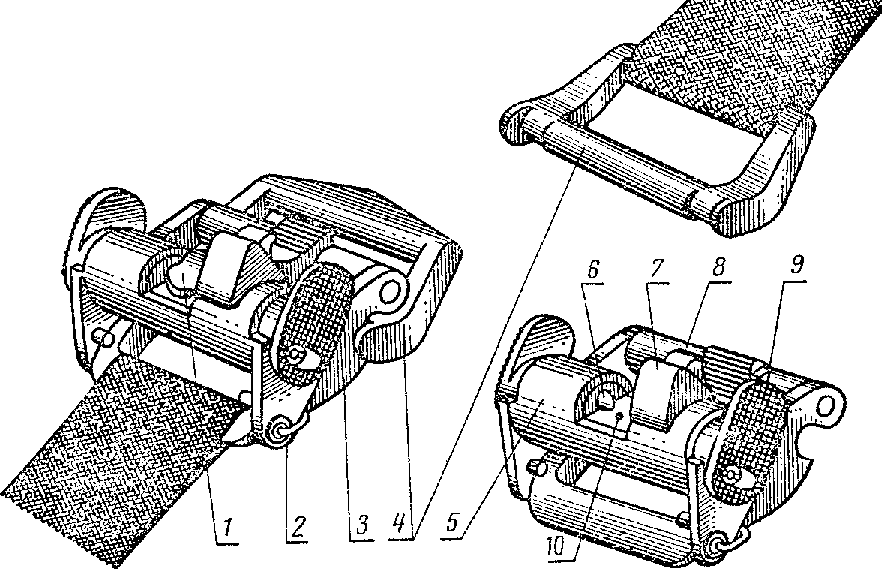
\includegraphics[height=3in] {images/20}
	\caption{����� ���:}\label{ris20}
	{\scriptsize 1~--- �����; 2~--- �������; 3~--- ������; 4~--- ������;
	5~--- ������ �����; 6~--- �����; 7~--- ������ ��������������;
	8~--- �������� ��������������; 9~--- �������;
	10~--- ���������� ������� �����

	}
    \end{center}
\end{figure}

{\bf ����� ���} (���.~\ref{ris20}) ������� �� �������, ������, ������� �����,
�������, ������ ���������� ����� ��������� �������, ������ � ����� �������,
������ ��������������, ��������� �������������� � �������.

����� ������� �����, ���������� ������ ���������� ����� �������� � ������
��� ������ � ������� �����, ����� �������������� �� ����� ����� ������.
����������� ������ ����� ������, ����������� � ������, ����� ������ ��
������� � ������� ����� � ������� ������ � �������. ������� ����� ������
������ � ������� � ������� �����, ���� ������� ����� ������ ��� ���������
������� �� ����� � ��������� �������. ������ ������� ��� ���� ������ �����
� ��������� �� ����� �������� ����� ������. �������������� ������ �� �����
����� ����� ��������� �������������� ��������� ������� �������. ����������,
��� ������ ������������� �����, ��������� �������������� � ������� �������
���������.

��� ������������ ��������� ������ ��������� ������� ����� ������ �� ��������
�������������� � �������� ������ �������������� � ������� ������ ���������.
����� ������ �� ��� ������� � ������� ������ ����� � ������� ���� �� ������.
��� ���� ����� ����� ������ �� ���������� � �������������� ������������ �����
� ���������� ������ ����� �� ��������� ������ ��������� �������. ���
���������� ������� ����� ���������� ������� ����� �� ������ � ������� �����
������ ���� �������.

\begin{figure}
    \begin{center}
	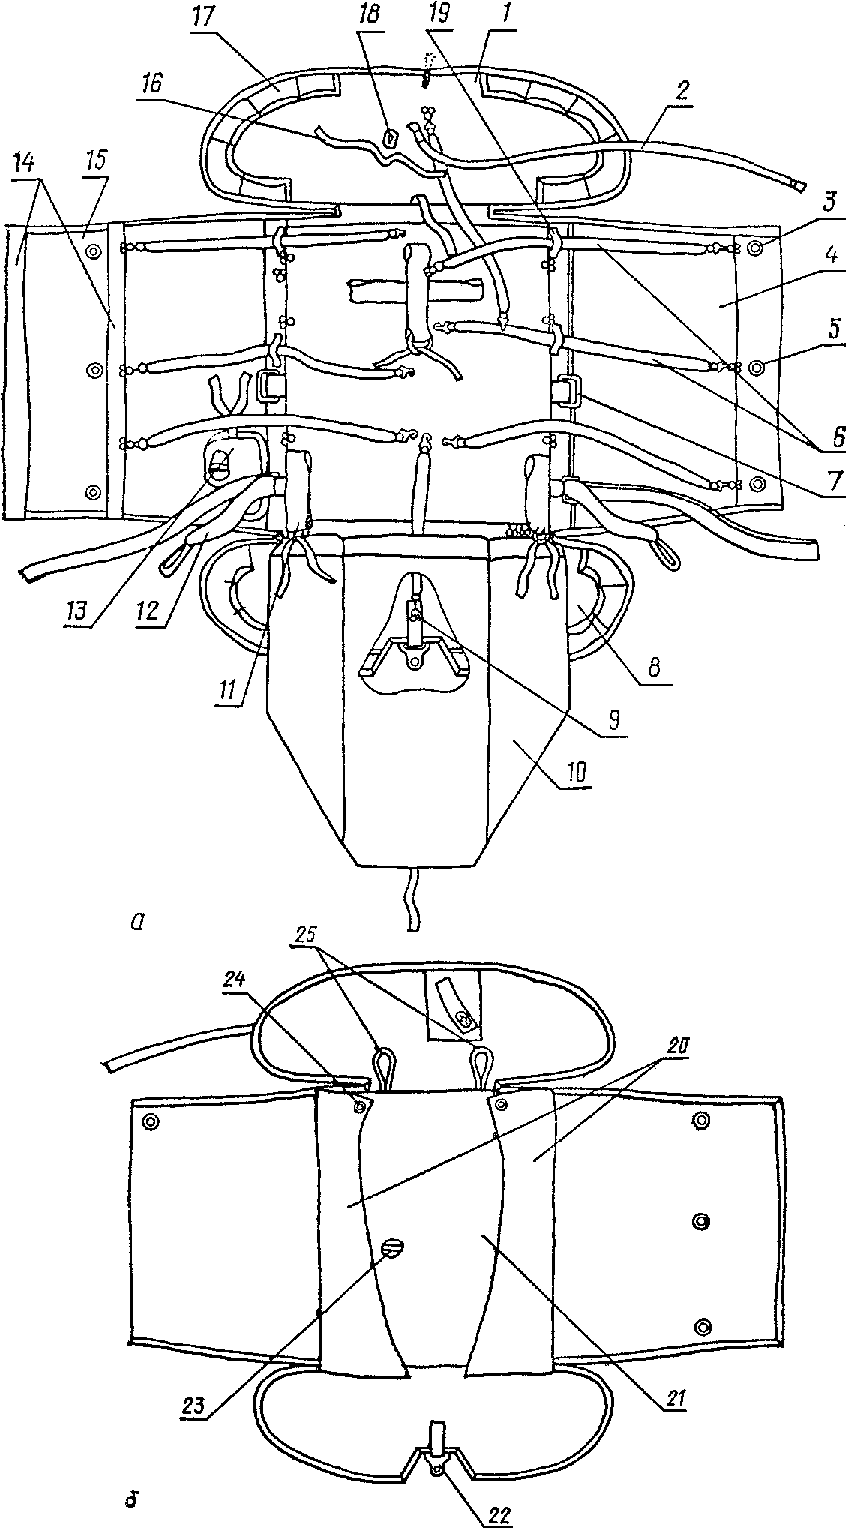
\includegraphics[height=6.8in] {images/21}
	\caption{����� �������� ��-15 ����� 5:}\label{ris21}
	{\scriptsize �~--- ��� � ������� �������; �~--- ��� � ���������� �������;\\
	1~--- ������� ������; 2~--- ������ �����; 3~--- ������ � ���������
	������; 4~--- ������� ������; 5~--- �����; 6~--- �������� �������;
	7~--- ����� � �������; 8~--- ������ ������; 9~--- ����������� �����;
	10~--- ������; 11~--- ����� ��������� ��������� ������� � �����;
	12~--- ��������� ��������� ��������; 13~--- ������ �������;
	14~--- ����������� ��������; 15~--- ����������������� ������;
	16~--- �����-�������; 17~--- ������; 18~--- ������� ��������;
	19~--- ������; 20~--- �������; 21~--- ��� �����; 22~--- ������-������;
	23~--- ���� ���������; 24~--- ������; 25~--- ��������� ����

	}
    \end{center}
\end{figure}

{\bf �����} �������� (���.~\ref{ris21}) ���������� �� ����������� �������� �
������� �� ��� � ������� ��������: ���� ������� (������� � ������), ������
�������� � ������ �������.

��� ����� �������, ������ ��� ������������ ���� ���������. �� ������� �������
��� ������� ���������� � ����� ��� ��������� ����� � ��������� �������,
����� � ������, ������� �� ��������� ��� �����, ��������������� ��� ����������
� ��������� �������� �����. � ������� ��������� ��� ������� ������ ������.

� ���������� ������� ��� �����, �� ������� � ������ �������� ���������,
������ �������, �������������� �������� ���������� � ����� ������ �� ���
����� � ������ ��������� � �������������� ���������������� ����������� �����
� ���������, � ���� �������. �� ���������� �������� ������� ��������
�������� ����.

� �������� ������� ����� �� �������� ���������� �������, � �������
������������ ��������� ����, ���������� ������ �����. ������-������� ����
�������� � �����, �������������� � ������ ����� � ���� ���������. ���� �
����� ��������� ��� �� ������ �������� ��������� ����.

�� ������� ������� ��������� �����, �������� ��������� ������, ������� ���-�,
�����-�������, ����� ������� ������ � ����� ��� ������������� �������� ������.
� ������ ���������� � ���� ����� ������� ������ ����� ������, � ������� ���
������� ������ �������� ��������� ����� ��������� �������.

�� ������ ������� ������ ����� ��� ������� � ������-������.

������� � ������ ������� ����� �������� � ���������, ������� ����� �������
������ � ����� ������������ ��� ������� �������. �������� ������������ �����
�� �����������.

�� ������ ������� ������� ������ ���� ��������� ������� ������� ���-� �
������-�������� � ��� ����� ��� ������������� �������� �����. ������ �����
��� ������� ��� ��������� ����� � ����������������� ������, ������� ����������
����� ��������-����������� � ������������ ������� ����� �������������
�������������� �� ��������������� ����������.

�� ����� ������� ������� ������ ��� ����� ��� ��������� �������� �����. ������
����� ���� ������ � ��� ������ ��� ��������� �����.

�� ������� ������� ����� � ������� ������� ����� �� ��������� ������ ������
������ � ������� ��� ������������� ��������� �������� � �������� ���������
������� � ��� ������������� ��������� ���������� �������� � ���� �����������.

��������� ��������� �������� � ������� ���� ������ ����������� ������������
����� ����������� �������������� �������, � ������ ���� ������~--- ���
������� �� �������� �����������.

�������� ������� �������� ������, ����������� � ������, � ���������, �������
��������� �� ����� �� ����� ��������� ��������.

�� ��������� ��-15 ����� 5 ������� � ��������� ��������� ����� �����������
�������� ������. ����� �������� ������ � �������� �� ������ � ������� ��������
����� 335 ��. �� ������� ������ �������� ������� �������� ������ ������ 385 ��.

{\bf ������ �����} ���������� �� �������������� ������� ������ ������ 515 ��,
���������� ���������� ������. ����� ������ � ������ ���������� � �������������
��������. ������ ����� ����� ������ ���������� � �������� ������� �����,
������~--- � ��������� �������, ���� ����� ��� � � �������������� ��� �����.

\begin{figure}
    \begin{center}
	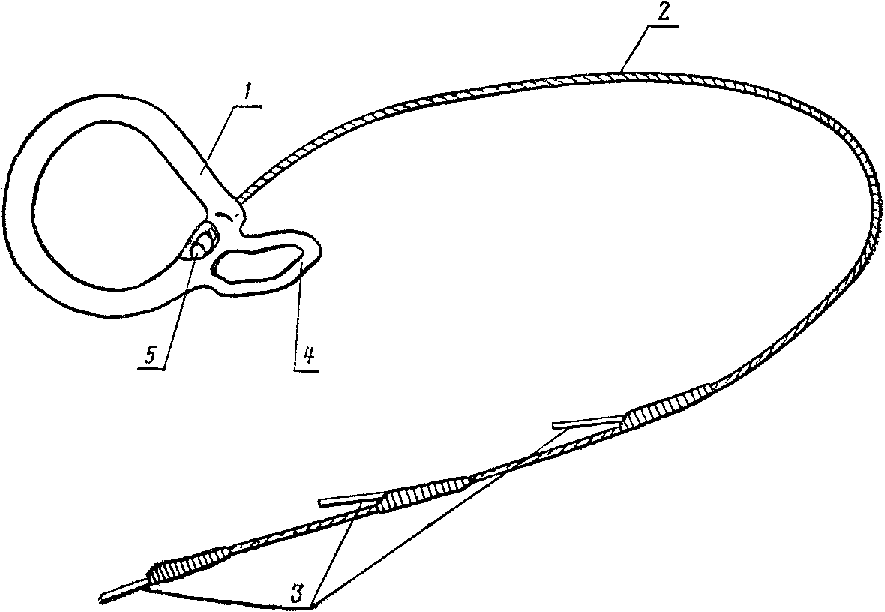
\includegraphics[height=2.5in] {images/22}
	\caption{������������ �������������� �������� ��-15 ����� 5:}\label{ris22}
	{\scriptsize 1~--- ������ ��������� ������; 2~--- ����;
	3~--- �������; 4~--- �����; 5~--- ������������

	}
    \end{center}
\end{figure}

{\bf ������������ ��������������} (���.~\ref{ris22}) ������� �� �������,
������, �����, ����� � ����� ��������� � ������������� � ��������� ����.
������ ������ ���������� �� �������� ������ ��������� 10 ��. �� ������������
� ������, ������������� �� ����� �������� ����� ��������� �������. ���
�������� ������� ����� ������ �� ��������� � ����� �������� �� 135${}^\circ$.
������� ��� ��������� ����� ����������� ���� �� ������ �� ���������� 150 ��.
������ �� ������� ������� ����� ����� 38 �� ������ � ������~--- �� 32 ��.
����� ����� �� ����� ��������� �������~--- 1070 ��.

\begin{figure}
    \begin{center}
	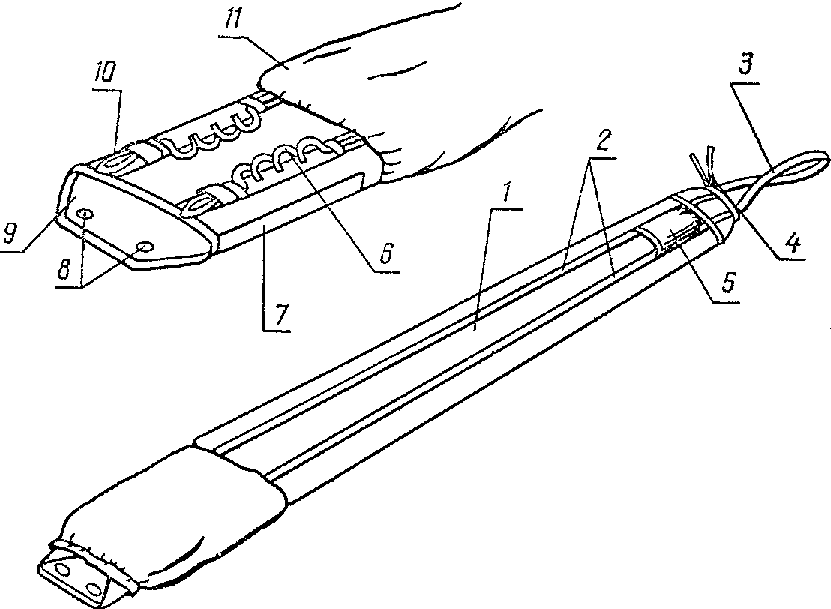
\includegraphics[height=2.8in] {images/23}
	\caption{����� ������ �������� ��-15 ����� 5:}\label{ris23}
	{\scriptsize 1~--- ������ �����; 2~--- ����� ������������;
	3~--- �������; 4~--- ����; 5~--- ������; 6~--- ���������
	��������� ����; 7~--- ����� �����; 8~--- �������; 9~---
	������ ����� �����; 10~--- ������� ��������� ����;
	11~--- �������������� �����

	}
    \end{center}
\end{figure}

{\bf ����� ������} (���.~\ref{ris23}) ����� ����� ������ ������ 3,37 �.
�� ���� ����� �� ������ ����������� �������, ������� � ������� ����� ��������
������� ��� ��������� ��������������� �����. ����� ������� ����� ���������,
��������������� ������ ����� �� ��� � ���������� ��� � ������. ������� �����
����� ����� ������� ������ ������������ ������ � ������������.

� ������ ����� ����� ����� ������ � ����� ���������, ���� ���� ������� �
������ ���� ��������� ��� � ��� ����� ��� ��������� ���������� ����. ���
��������� � ������� ������� ������� ��� ������� � ��� ������ ����� �����
��������� ������� �����.

������ ����� ����� ����������� ����� ������� ����� ���������������,
�������������� ����� �������������� �����, ������� �� ��������� ������.
������ ����� �������������� ������� ��������, ����������� � ������ ������.

\begin{figure}
    \begin{center}
	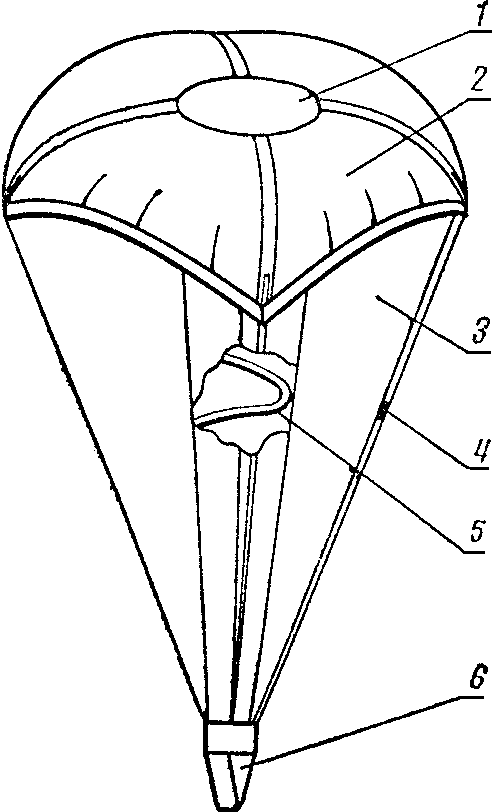
\includegraphics[height=2.3in] {images/24}
	\caption{�������� �������:}\label{ris24}
	{\scriptsize 1~--- ��������; 2~--- ������ ������; 3~--- �����
	� �������; 4~--- ������; 5~--- �������; 6~--- �������

	}
    \end{center}
\end{figure}

{\bf �������� �������} (���.~\ref{ris24}) �������� 0,4 �${}^2$ ������� ��
������ ������ ���������� �����, ������, ������, ������������� �� �������, �
������� ��� ����� �������� � ��������. �� ��-15 ����� 5 ����������� ���
�������� ��������.

��� �������� �� ������ ������ � ���������� ������ ������ ���������� �����.
�� ����� ����� ��������� � � ������ ��������� ���������� ������, �����
������� ��������������� � ������ ������. ������ ������, ����������� ������
�����, �������� ������� ��� ��������� � ��������������� �����. ������ ������
�������� ��������� ���������� �������, ������� ������ ����������� �������
��������� �� ����������� ��������.

\begin{figure}[!hbt]
    \begin{center}
	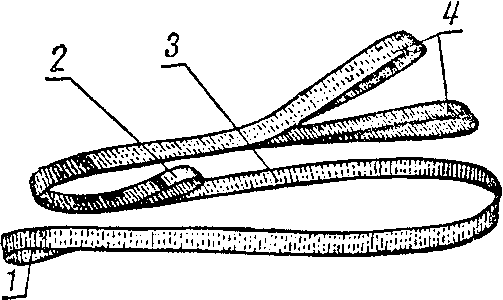
\includegraphics[height=.8in] {images/25}
	\caption{�������������� �����:}\label{ris25}
	{\scriptsize 1~--- ����� ��� ������������� � ����� ��������������
	�����; 2~--- ����� ��� ������������� � ������� ������; 3~--- ����;
	4~--- �����, ��� ������������� �������� ���������

	}
    \end{center}
\end{figure}

{\bf �������������� �����} (���.~\ref{ris25}) ������������� ��� ����������
������, ����� ������, ����� ����� � ���� �������� ���������. ���������������
�� ����������� �����, �������������� ������ 550~���. �� ����� ����� �����
������� �����, ������� �������������� � ����� �������������� ����� � �
�������������� �������. �� ���������� 0,75~� �� ��� ��������� ������ �����
��� ������������� � ����� ������. �� ���������� 0,33~� �������������� �����
������������� � �������� ��� ����� ��� ������������� �������� ���������.
��� ���������� ����������� ������-�������. ����� ����� 1,4~�.

\begin{figure}[!htb]
    \begin{center}
	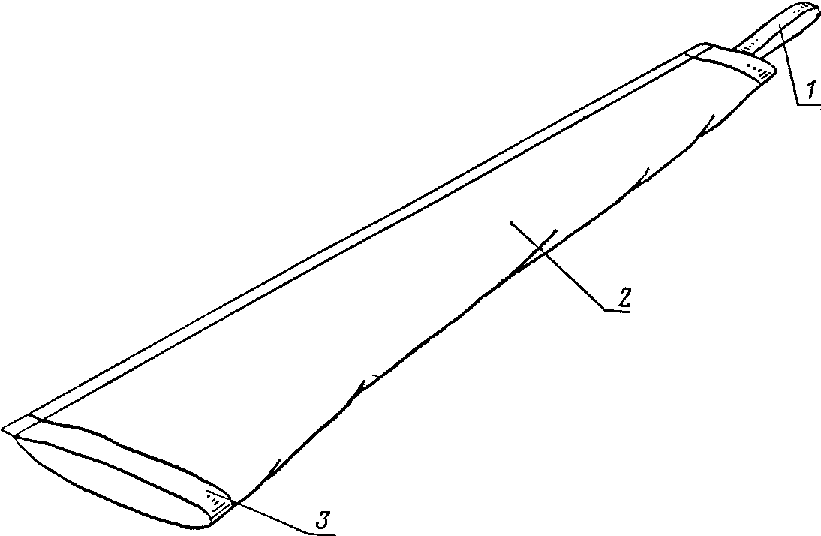
\includegraphics[height=2.2in] {images/26}
	\caption{����� ����� �������� ��-15 ����� 5:}\label{ris26}
	{\scriptsize 1~--- �������; 2~--- ���������; 3~--- �����}
    \end{center}
\end{figure}

{\bf ����� �����} (���.~\ref{ris26}) ������ ��� �������������� �����������
�������������� ����� ��� ������� �� ������ � ������ ��������������� �����.
�� ������� �� ����������� ���������, �������� ����� ������ ������ 1,5~�,
� ������� ��� ������������� � �������������� ������� ������. ������ �
������� ������ ����� ������� ������.

\begin{figure}[!bht]
    \begin{center}
	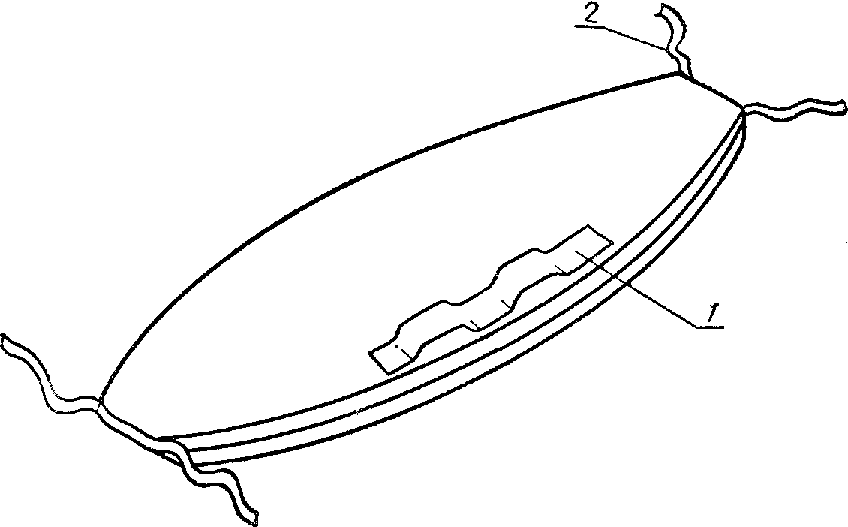
\includegraphics[height=2in] {images/27}
	\caption{������� �������� ��-15 ����� 5:}\label{ris27}
	{\scriptsize 1~--- ����� ��������� � ������ ��������; 2~--- �����-�������}
    \end{center}
\end{figure}

{\bf �������} (���.~\ref{ris27}) ������������� ��� ������������� �����������
�� ������ � ������ �����������. ��� ����������� �� ����������� ���������
�������� 40--50~��, ������� ���������� ���������. �� ������� ������ ������
��� ��������� � ������ �������� � �����-������� ��� ��������� � ���������
�������.

�� �������� ����������� ������ ���-�, ������� ���������� � ������ �����������
�������� �����, �������������� ��� ������ ��������� ����������� � �������
�������.

��� ���������, �������� � ��������������� ������� ����� ����������� ����������
�����.

{\it ������ �������� � �������.} ������� ��-15 ����� 5 ������� � ������ ���
������� �������� ���������� ���� ���������� �� ��� ������������ � ������� ��
��������� ������ ��������:\\
\mbox{\quad}�� 120 �� 225 ��/� � ������ �� ���� 150 � ��� ����������� ��������
�������� � ��������;\\
\mbox{\quad}�� 225 ��/� � ������ �� 1000 � ��� ����������� ��������� �������� � �
��������� � ���������;\\
\mbox{\quad}�� 240 ��/� � ������ �� 2000 � ��� ����������� ��������� �������� � �
��������� � ���������.

������������ ���������� ��� ������� � ��������� � ��������� �� ��������� 16
������. ������� ������������ �������� �������� �� ������� 30--35~� �� �����
��� ����� ����� ���������� �� ����� 100 �� ���������� 5,1~�/�.

������� ��-15 ����� 5 �������� ��� ��������, ����������� ����� ��������
����������. ������ �������� �� $360^\circ$ � ����� ������� ��� ���������
����� ������ ��������� �� 5~�. �������������� �������� ������ ���������� 5~�/�.
����� �������� ��������� ����� ����� ���������� �������������� ��������
������ ����� �������� �� ����. � ��������� �������-���� ��� ������������ �
�������� ������������ ���� �������� ���������. ��-15 ����� 5 ��������
��������� ��� ������������ �� ����� $10^\circ$ �.

\chapter{������� ���������}

\section{����� ���������}

������� ��������~--- ��� ���������� ��� ��� ���������� � �������, �������
������ ���������� �������� ������ �������� � ��� ��� ���� �������� ���������.

���� ������� ���������� ��� ��������~--- ������������ � ����������~--- ���
������������ ��������� �������� ����������� ���������� ����������.

�������� ���������� �� ����������� ���������� ������ ������ 12--15 �, �������
1--1,2 � � ������� 1 � ��� �� �������� ����������. ����� ��������
�������������� ���������� � ��������������� ��������������: �������~-- 5 ��.,
�������~-- 3 ��., ���������� ������, �������, ����, ������, ����-�������,
����� ��� ��������� � �����������.

��� ������� ������� ������������ �������� ����� ���������� ��������������� ��
���������, � ������� ��������, � ���������� ���������� ��� ����� �����.
����������� ��� ������� �������� ������� �� ����������� ��������� � ���������
������������ ����������� �����������. ����� �������� ��������� � �������
������, ��������� ����������� ���� �� ����� ���������� � ����������� �
10--15 ��. ��� ������ ����� ����� �������� ������������ ��������� �� �����
���������������� ����� �������� $4,\!5\times 2$ �, ��������������� ���
������������� ������ �� �����������.

������� ��������� �������������� �� ���� ������:\\
\mbox{\quad}������ � ���������� � �������;\\
\mbox{\quad}������� ������;\\
\mbox{\quad}��������� ����� �� �����, ������� ����� � ����;\\
\mbox{\quad}������� ������ � ����� �� �����;\\
\mbox{\quad}������� �������� �����.

������ ��� �������� ����� ���� �������� �������, � ����������� �� ������� �
������������ ��������������� ���������� � �������.

������� �-1-5-� ����� ��� �������� �������: ���������� ����� � ���������
������ �������� �����, �������������� ���������� ����� �������� �����,
������ ��������� ��������.

������� �-5 ���������� ������ � ����� ��������~--- � ������ ���������� �
���������� ��������� �������� ���-�.

������� ��-15 ����� 5 ����� ���� ���� ������� �������~--- � ������ ����������.

���������� �������� ������� ������� �� ���� ���� ����� ���������.

\section{������� �������� �-1-5-�}

\subsection{������� �������� �-1-5-� � ������� ���������� ����� �
��������� ������ �������� �����}

{\sc I ����.} {\bf ������ ��������.} �������������� � ���������
������������������: �����, ������, ����� ������, �������� �������, ���������
�������, �����, ������������ ��������������, �������� ���, ���������� �����.

{\it ������ ������} �������� � ��������� �������� ����� ������ � ����� �
����������� ������ �� �������� �� ��� �����.

����� ���������� ����� � ������ ������ 1-� � 2-� ������, �������� �� �� ������
��������� � ����������.

������������ �������� ������ ����� � ����, �������. ���. ���� ���������: ��
��������� �� ������� ������ ����� �������� ���������, ��� �� ������� ����� �
�������������� �����, �� ���������� �� ������� �������� � �����, � �����
��������� ��������� ����������� ��������� ���������.

���������� � ��� ����� ��������� ��������� ��������� ����� � ������.

����� ������� ������� ����� 1-� � 2-� �������� ���������� � ������� �������
����� 2-� � 3-� ��������. ��� ����� ���������� ��������� 1-� ������, ����� �
����� ���� 2-�, � � ������ 3-�.

������������ �������� ������. � ����� �� ������� ��������� ������� �����
���������� ��������.

{\it ������ �����.} ������ ������ ���� � ������ � ����������. ����������� ��
������ � ��������� �������, ������������ ����������� ������, � ����������
������������ ������������� ������� ����� �, ���������� �� ����� ��������,
������� ����������� ��������� �������. ����� ����� ��������� ����������
��������� ����� � ��������� �������.

{\it ������ ����� ������.} ��������� ����������� �����, ������� ������������
����, ������� � ��������� ��������� ���, �������������� �����, �������� ���
������� �����. � ������ ������� ��������� ���, ��������� ������ ������ �����,
�� ���������� �������� ������. ������������� ��������� ���� �������������
�����������.

{\it ������ �������� ��������� �������� (���).} ������� ������� ����������
������������ ����� ��������. ���� � ���, ��� ������� ���������� ����������
���������� � �������� ������������ ����������� ������������������ ����� � ���
��������� ��� � ����� ������� ��� ��������. �� ��������� �����, � ����� ���
�������������� ������������ ����� � �������� ������, ��� ����� �������� �
������� �����, ������� ����� ����������, ������ �� ������ ��������������
�����������.

����� ���� ���������, ��� �� ����������� ����� � �����, ������� ������� �
����������� ������, ����������� ���������� ������� � �������-���� ���
��������� ���������� ���.

��� ����������� �������������� �������� ������� ��������, ��� ��� ����
�������� ������������� ����� �������� � ���������� ��� �� ������ ����� � �
����������� \flqq����\frqq~--- �������� �������� ������ � ������ ��������.

{\it ������ ��������� �������.} ��������� ��� ������������� ������: ����� ���,
����� ��������� � �����������, ��������� ������, ��������. �������������, ���
�� ����������� �� ������ ������-���������, ����� ������� �������� ������
����������, ���������� ���������� ��������� ���������, ��������� �����������
������� ��������� ������.

������� ��������� ������� �� ������ ����� ���������, � ������~--- �����������.
�� ����������� ������� �� ������ ���� ����� �� ���������, ����������� �����.

{\it ������ �����.} ��������� ����������� � ���������� ��������� ��������,
�������, ��������� ������, ����������� ������ ��� ��������� �������� �����,
��������� ������ �������, ����-�������, ������� ��� ������� �������������������
���������, ������� � ����������� ���� � ��������� ��� ��������� � ������������
��������� ��������.

� ������ ���������� ��������� ������ ��� ��������.

����� ����� � ��������� �� ������ ����� ��������� ������� � �������. ��
����������� ����� ����� ����� �� ����.

��������� ���� �� ������ ����� �������� � �����������. ����������� ����
�������� ������.

������ ������������ ������������� ��������� ����� ������� ��� ������ ������
�����. ������� �������� ��� ����������� ����� �����������.

{\it ������ ������������� ��������������.} ��������� ��������� ����� ������,
��������������� �����, ������ � ����� �����.

���� �� ������ ����� ������ �������, ����~--- ��������.

��� ����������� �������������� ������������ �������������� ���������� ��������.

��������� ����� ����������� ������������������ ����� ����� ���������������
���������~--- �� ���������� ����������� ����� ����� � ��������. ��� �����������
�������������� ����� �����������.

{\it ������ ��������� ����.} ���������, ��� �� ����������� ��������� �����
����� � �����, ���������� ������� �� �������, ���������� �����. ����� �������
�� �������������� � ������� ��������� �� �����������.

{\it ������ ���������� �����.} ���������, ��� �� ����� �� ����������� �����
���������, ������� ����� � ��������� �������, � ����� ������� ������-���������
��� ����������.

\begin{figure}[!b]
    \begin{center}
	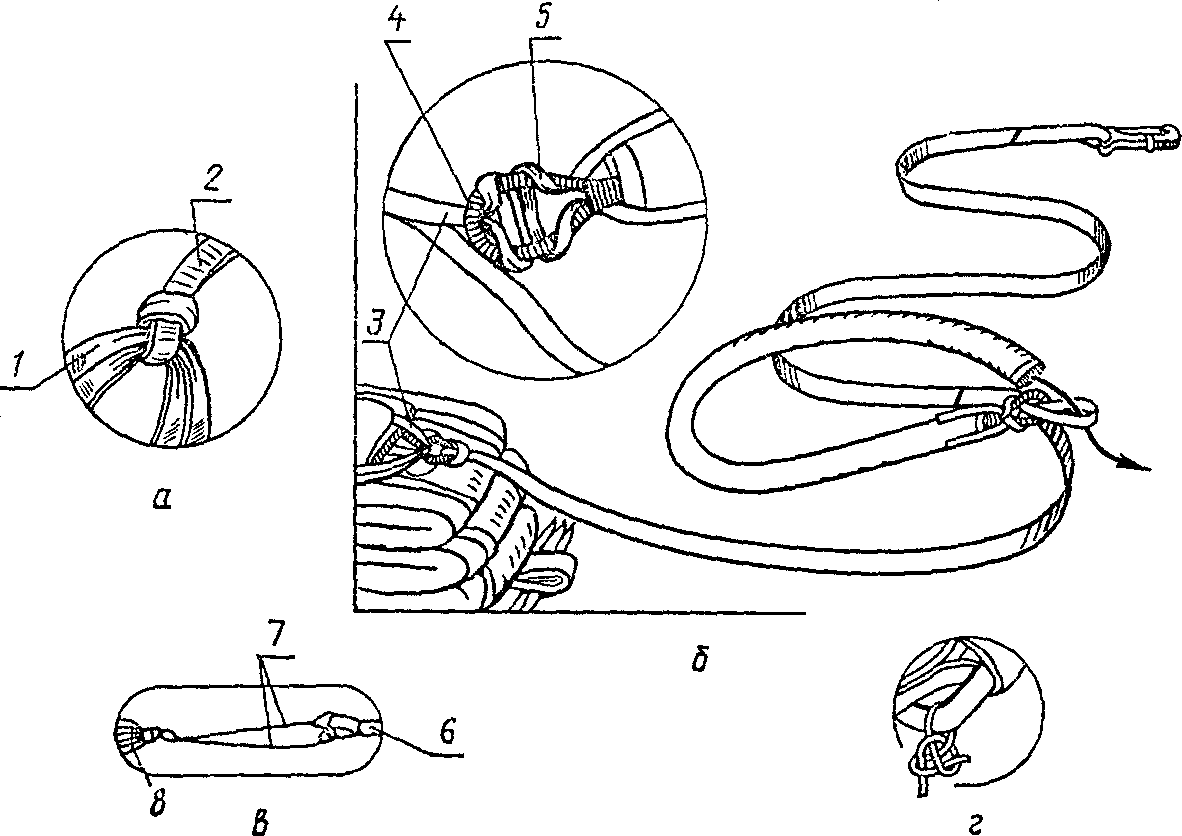
\includegraphics[height=3in] {images/28}
	\caption{������� �������� �-1-5-�:}\label{ris28}
	{\scriptsize �~--- ������������� ��������� ���� � ������� ����� ������;
	�~--- ���������� ��������� ����� � ����� � ������ ��������� ����;
	�~--- ������������� �������� ������ � ������� ������;
	�~--- ���� ����������� �������� ������;\\
	1~--- ������� ����� ������; 2~--- �������� �������; 3~--- �����
	�������� �������; 4~--- �������� �����; 5~--- �����
	������������������ �����; 6~--- ����� �������� �������;
	7~--- ������ �������� (�������); 8~--- �����

	}
    \end{center}
\end{figure}

{\bf ���������� � �������} �������������� � ��������� ������������������:\\
\mbox{\quad}� ������� ����� ������ ������������ ������-������� ����� ���������
���� (���.~\ref{ris28},�);\\
\mbox{\quad}�������� ���� ��������������� ��������� ��������� � �����������������
�����. ��������� ����� ����� � ��������� �����, ��������� �� ������-������� ��
������� ������ �� �������� ���� (���.~\ref{ris28},�);\\
\mbox{\quad}������������ �������� ������ � ������� ������ (���.~\ref{ris28},�);\\
\mbox{\quad}����������� ���������� ����� � �������� ����� ��������� ���� ����������
������� � �������� ����� �������� ������ (���.~\ref{ris28},�).

{\sc II ����.} {\bf ������� ������.} ����� �������� ������� ������ �������� ��
������� ����� ��� �� ����� (� ������� ��������). ����� ����������� �� ���
�����.

��������� ������� ������ ���, ����� ��������-�������� ������� ���� ������.
������ ��� ���� ������ �������� �� ����� � ������ ������, � ������ ������~---
�� ������� � ������.

�������� ������������ ������������ �����, ���������� ����� 14-� ������
(� ������� ������), ���������� �� �, ��������� �� �����, ������������� �����
�������� ������ �� ������ ������� �����, ������ 15-� ������ �� 14-�, �
������������ ������������ ��������� ����� �������, ����� ������������
��������� �����, ��������� ����� ������, ������� ������������ ������ �� �����
������ (���.~\ref{ris29}).

\begin{figure}[!hbt]
    \begin{center}
	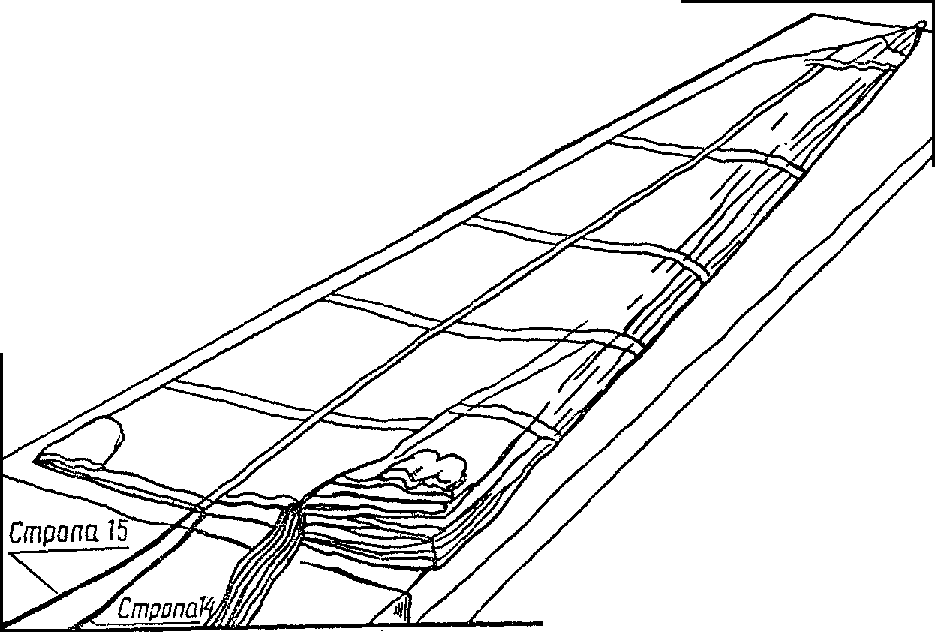
\includegraphics[height=3in] {images/29}
	\caption{������� ��������}\label{ris29}
    \end{center}
\end{figure}

���������� ���������� ��� ��������� ����� �������� ������ ������ �� ���������
� ������� ������-������������.

\begin{figure}
    \begin{center}
	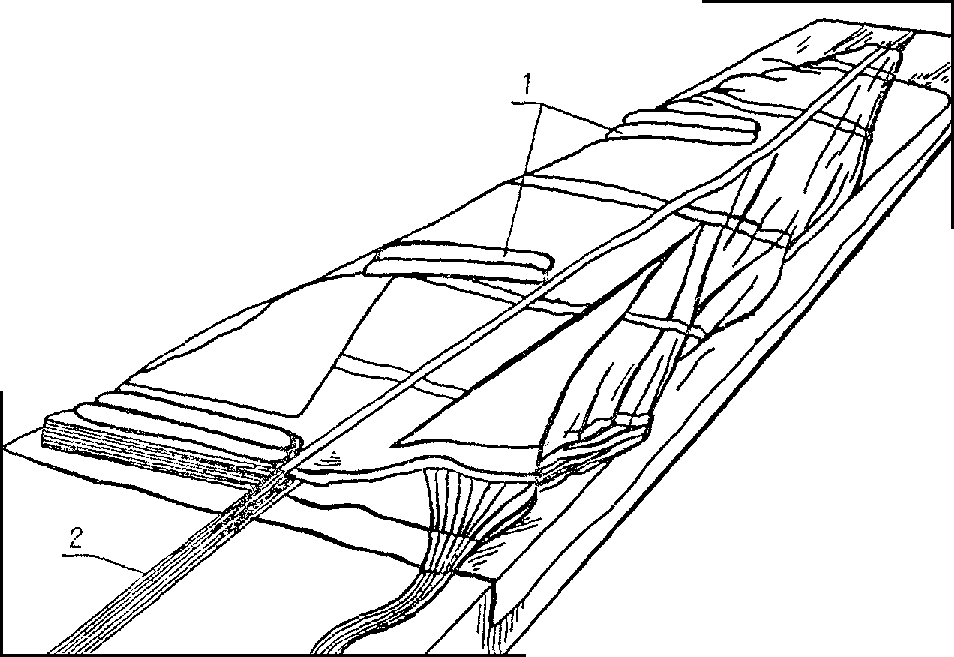
\includegraphics[height=3in] {images/30}
	\caption{��������� �������� ������:}\label{ris30}
	{\scriptsize 1~--- �������; 2~--- 28-� ������}
    \end{center}
\end{figure}

����� ����� �� ��������� ����� ������ ������ ������-���� ��������
(���.~\ref{ris30}), ������ �������� ������ ������������� �� ��������� �����
��������, 14-� ������ ��������� ������ � �� ��� ���������� ������ ������
������ �� ��������� � �������. ��������� �����������, ��� � � ����� ������.

��������� � ����������� ���������� ��� ��, ��� � ��������� ��� ���������.

��� ���������� ������� ����� ����� ��������� ����� � ����� ������, � ������
����� � ����������� �������~--- � ������.

����� ������� �������� ������� � ����� ������� �������, � ��������� ������
���������, ��� ��� �������� �� ���.~\ref{ris31}.

\begin{figure}
    \begin{center}
	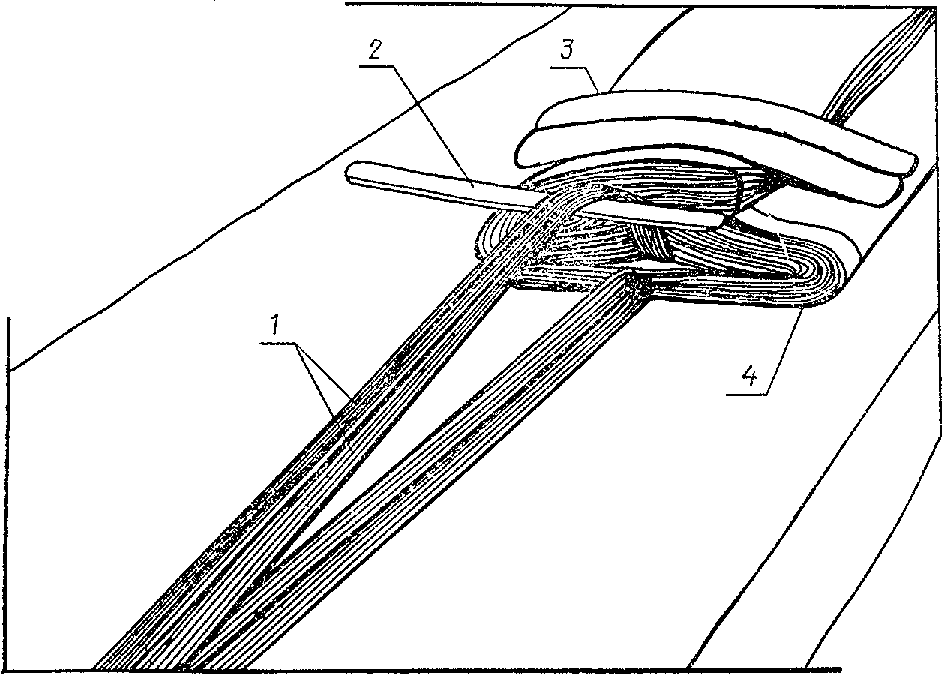
\includegraphics[height=3.3in] {images/31}
	\caption{���������� ��������� ��������:}\label{ris31}
	{\scriptsize 1~--- ������ ������� ���� ��������� ������
	��������� �������; 2~--- ���������� �������; 3~--- ������;
	4~--- �����

	}
    \end{center}
\end{figure}

����� ������� ������ ��������� ������������ ��� �������. ��� ����� ������
����� �� ����� � ������ ������. � ����� ������������� � ������ ������ ��
������ ���������������.

\begin{figure}
    \begin{center}
	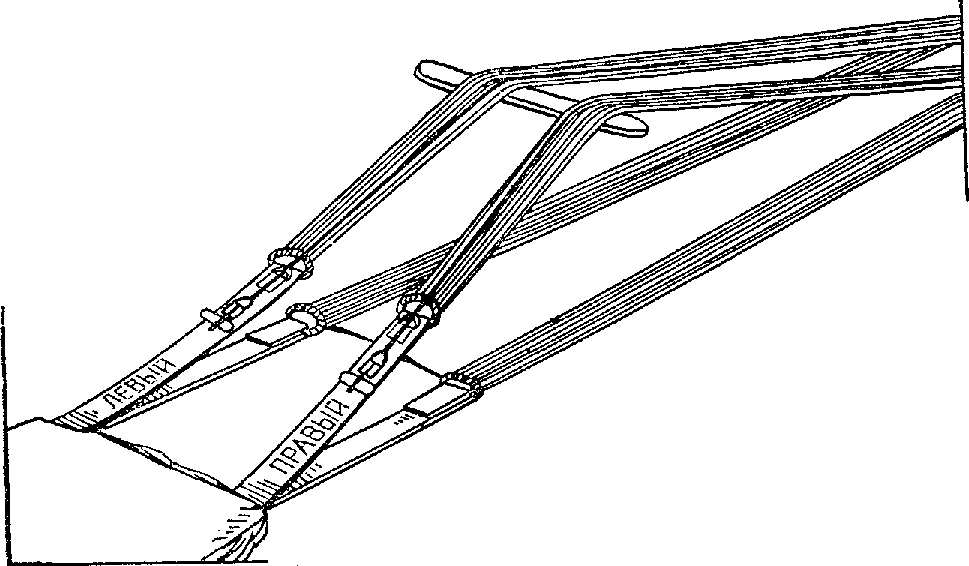
\includegraphics[height=2.8in] {images/32}
	\caption{������� ����� ��� �������� ������������ �������}\label{ris32}
    \end{center}
\end{figure}

����� ������ ������ ����� ����� �� ������� � ������. ������ ��� ���� �����
�� ������ ���������������. ��������� ��������� ����� ������� ��
���.~\ref{ris32}.

{\sc III ����.} {\bf ��������� ����� �� �����, ������� ����� � ����.} �������
� ������ ������� � ����������� ������� ������ �� ������� ����� ��� �����.
��������� ���� ������ �����, �������� �������������� �������������� �����,
�������� ����� ��������� � ������� ����� �� ������� ������ (���.~\ref{ris33}).
����� �� ������ ������ ����� � ���������� ��� �� �����. ��������� ����������
���� � ������������ ����� �� �����. �� ���������� 0,5 � �� ������ ������ �����
����� ����� � ������ �� �� ����� ������ ����� ������ (���.~\ref{ris34},�).
��������� �������� ������ ������ ������, ��������� ������� ������� ���� �
��������� �� ������� �����, ����� ����� �����, ������� ��� �� ����� � ���
������ ������ ������������ ������ ������� � ������, � ����� � ����� �������
����. ����� ����� �����, ��������� � ������� �����, ������� ��������� �������,
����������� ��� �������������� ���������������� ������ ����� �� ������� ��� �
������ ������ ����� � ������� �� ����� (���.~\ref{ris34},�).

\begin{figure}
    \begin{center}
	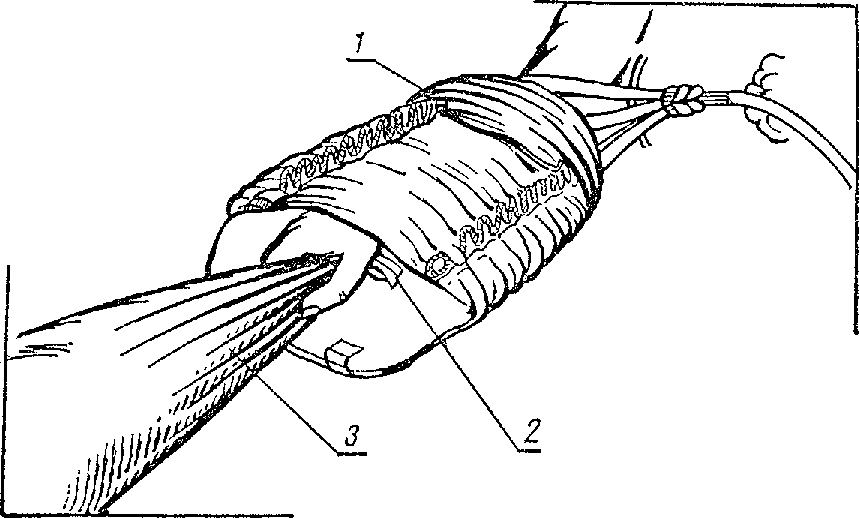
\includegraphics[height=2.8in] {images/33}
	\caption{��������� ����� �� �����:}\label{ris33}
	{\scriptsize 1~--- ����� ������; 2~--- ������� ������; 3~--- �����}
    \end{center}
\end{figure}

\begin{figure}[!hbt]
    \begin{center}
	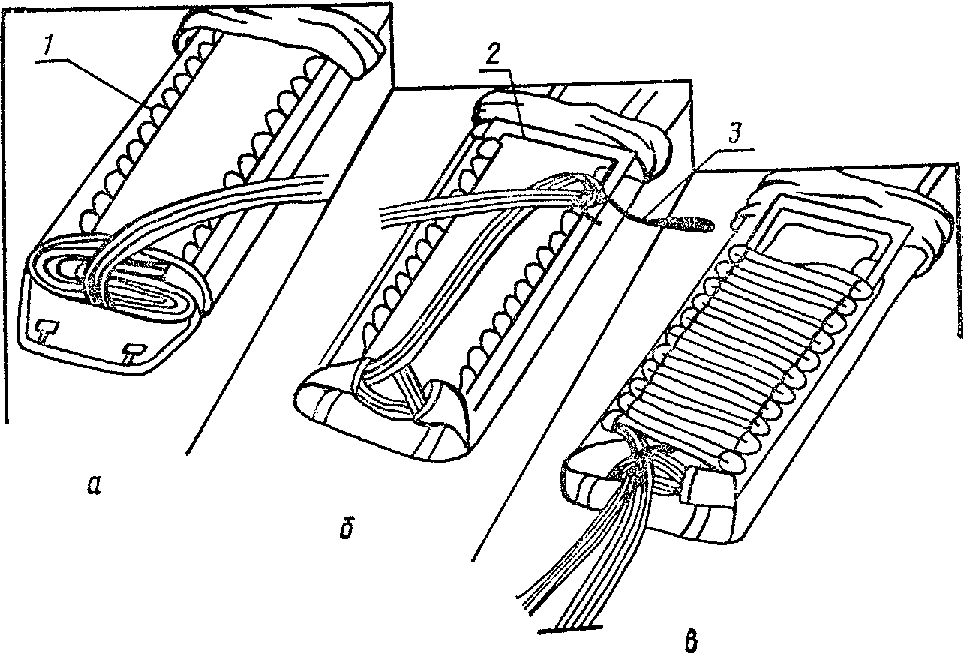
\includegraphics[height=3.3in] {images/34}
	\caption{������� ����� � ����:}\label{ris34}
	{\scriptsize �~--- ������ ������� �����; �~--- ��������� ������� ���;
	�~--- ������� ����� ����� ������� � ����;\\
	1~--- ��������� ����; 2~--- ���������� �����;
	3~--- ������ ��� ������� �����

	}
    \end{center}
\end{figure}

���������� ������� ����� � ���� � ������ ������ ��� ����� �� �����.

�� ���� ������� ��������� ������� ����������� � ������.

� �������� ������� ���� �������� �������������� ����� (���.~\ref{ris34},�).
� ���������� ���������� ����� ��������� ������ ����� � ��������, ��������
���������� ����� � �������� ����������������� ����� �����.

\begin{figure}[!htb]
    \begin{center}
	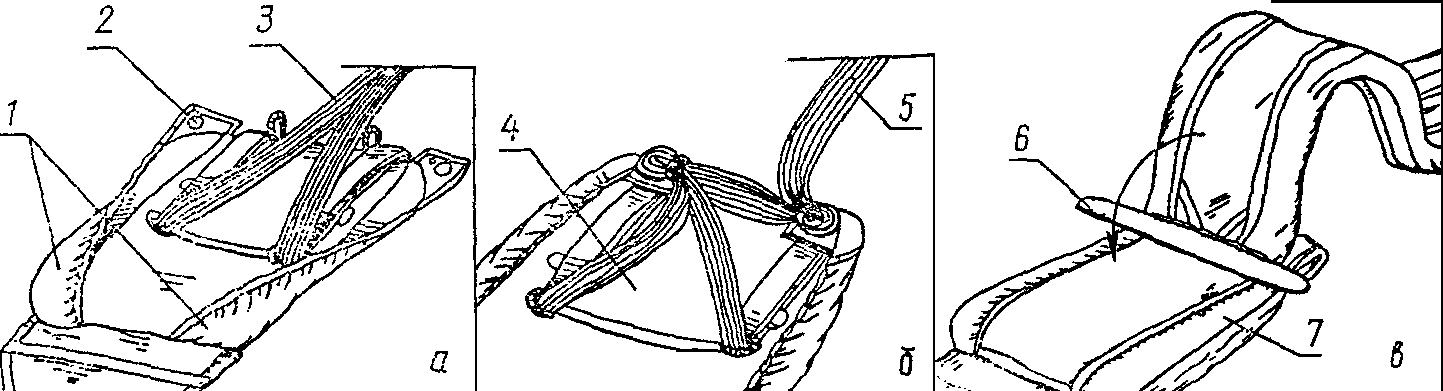
\includegraphics[width=350pt] {images/35}
	\caption{������� ����� � ������� � �����:}\label{ris35}
	{\scriptsize �~--- ������������ ��������� ������ ����� �������� ������
	� ����� �� ��� �����; �~--- ��������� ��������� ��� ��������;
	�~--- �������� ������ � ����� � �������;\\
	1~--- �������; 2~--- �������; 3, 5~--- ������; 4~--- ��� �����;
	6~--- ���������� �������; 7~--- �������

	}
    \end{center}
\end{figure}

{\sc IV ����.} {\bf ������� ������ � ����� �� �����.} ����� �������� �����
���������� ��������� �������� ��������, ��� ���� ���������� ����� � ����������
� ����� ������, ��������� ����� ��������� ������� ������� �� ��� ����� ���,
����� ������ ���� �� ������������� ����� ��������� ����� � ��������
(���.~\ref{ris35},�). ��� ���� �� ��������� ����������� ��������� � �������.
�������� ������ ��������� ��� ��������� �����. ��������� ���� ��������� �
��������� �������� � ������������: ������� �����, ����� ������
(���.~\ref{ris35},�).

����� ��������� ����� ����� � ����� ����������� �� ��� ����� ����� �������,
����� ������ ������ ����� ����� �� ���� ��� ����� � ��� ������ � ����� ������
������� �������. ������, ��������� � ����, ��� ���� ������ ���� ������.

�� ������ �������� ������ ����� �� ����� � ������� ����������� ����������
������� �, �������� �� ������ ���� ����� � �������, ����������� ������ ����.
����� ����� ��� ���� ���������� � ������� ����� (���.~\ref{ris35},�).

����� ��������, ��������� ��������, ���������� \flqq������\frqq{} ���������
����� ����� � ��������� � ���� �������.

��� �������� ��� ������� ����� � �������� ����� � ��������� � ���� ������ �
������� ���������� ����� ������ ����� ���� ����� � ������� ������ ���� ��
����� ������� ������ �����������.

�� ��������� ������� ������� ����� � �������� ����� ������ �������� � �������
����� �����.

\begin{figure}
    \begin{center}
	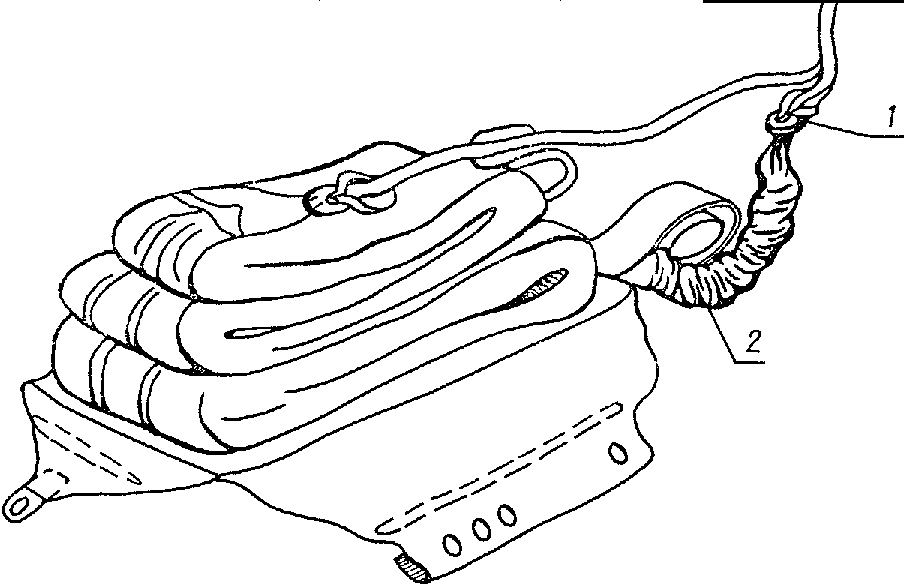
\includegraphics[height=2.8in] {images/36}
	\caption{����� � ����� ����� �������� �����:}\label{ris36}
	{\scriptsize 1~--- ���� ���������� ��������� ���� � �����;
	2~--- ����� � ������ � �������� ����� ����� �������� ��������

	}
    \end{center}
\end{figure}

{\sc V ����.} {\bf ������� �������� �����.} �� ������� ��������� �� ���� �����.
����� �������� ��������� ������������ ������������ ������� ������ � ��������
������ � ����� ��������� ����, �������������� � ����� ������. ����� � ��������
������ ������ ���� ������ � ������ (������ ������ ������ ��������� ������), �
����� ��������� ���� ������ ���������� ��� ���������� ������� ���������
������� (���.~\ref{ris36}). ����� ��������� ����-������� � ����� ���������
������, ������� ��� ����� �� ������ ������ ������ ������� �������� ��������
��������� � ����� ��������� ������ ��������������� �������. ����� �������
����� ����� �� ������� ������, �������� ������������ ����� ��� ������
�������� �������, ������ ����� �������� �� ����� �������� ������� �������
������ ������ ������ �������, � ����� ������ ������ ������� ������� � ���������
� ����� ������� ������� ��������� �����. �������� ��������������� ������� ��
��������� ������ � ��������� � ���� ������� ������� ��������� �����.

����� �����, �������� �� ����� ������ � ������� ������, �������� �� ������
����� ������ ������ ������� �������� �������, � ������ ����~--- ������-������
������� �������.

����� ������� ����� ���������� �������� ��������, ������� ���������������
����� � �������� ��������� ����. ����� ��������� ��������� ���� ���� ����������
���� � �������� ����� ������ � ����� �������� �� ��������� ������� �������
��-��� ������� ������ � ��������� � ����� ��������� �� ������. ���� ����������
��������� ����� � ���� ����� ������� ������. �������� ��� ���������� ��� ������
����� �������, ����� �� ����� ������� ��-��� ����� � ����� �� ������� ��.

����� ������� ��������� ������������ ���������� ��������� ���� � ������ ������
� �������� ������, � ����� ������������ ��������� ������ ��������� ����� �
������� � �������� �����.

������ ������� ��������� ����� ��������� ���������������� ������ \symbol{"9D}
40 � ��� ��������, �� ��� ������ ���� ����� �������� ������� ������������
���������� ����������.

\subsection{������� �������� �-1-5-� � ������� �������������� ���������� �����}

����� �������� �������� �� ������ �������� ���������� � ������ ����������
�������������� ��� ����, ������������ �����������.

���������� �������� ��� ������ ��� ����������� ������������� �����������.

������� ������, �������� �����, ��������� ����� �� �����, ������� ����� �
���� ����� ���������� ��� ��, ��� � ��� ������� �������� � ������� ����������
����� � ������ �������� �����.

{\bf ���������� � �������} �������� �-1-5-� � �������������� ����������� �����
����������� � ��������� ������������������:\\
������������ ������-������� ������� ����� ������ � ����� ���;\\
\mbox{\quad}��������� ������ ����� ��������������� ��������� � ������ ���
������\-��-�������� ��������;\\
\mbox{\quad}��������� �������� ���� ��������������� ��������� � �����������������
����� �, ��������� ����� ����� � ������ ������������������ �����, ��������� ��
������-������� � �������� ������ �� �������� ����;\\
\mbox{\quad}��������� ���� ��������������� ��������� � �����, ����� �������� ��
���������� � ��������� �������. ����������������� ����� ��� ���� ������� �
\flqq��������\frqq{} ������ ������;\\
\mbox{\quad}��������� ������ � ������ ���������� ��������� � ������ ���������
������, � ���� ���������� � �����.

{\bf ������� ��� � ������� �����} ������������ � ��������� ������������������:
��������� ��� ������ ������ ����� � ��������� �������, ������� ��� ��� ����
�����, ����� ����� ��� ���������� ������ �������� ������� �� ������ �������
�����, � ��������� � ������ ������������� ����� �����. �������� ��� � �������
�������� ���������� � ����� ������, ���������� �� ���� ������ ������� ������
�����, �������� ������ ������ ������ ������� �������� ������� �� ����� ���,
�������������� ����� �������-���� �� ������, � ��������� ���������������
������� � ��������� ������ ������ ������� ������� �������� �������
(���.~\ref{ris37}).

\begin{figure}
    \begin{center}
	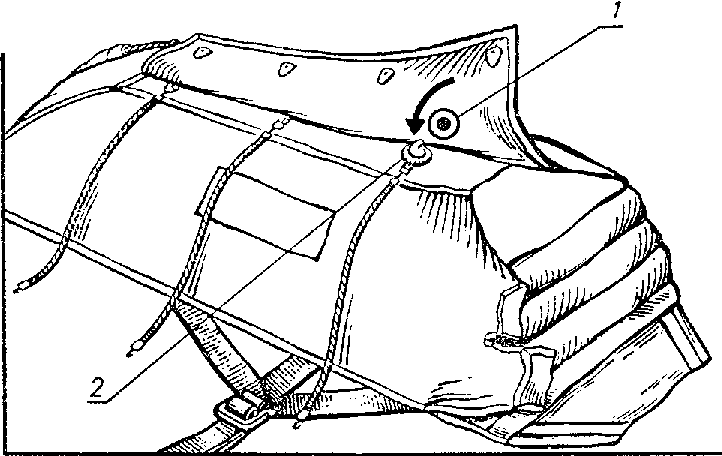
\includegraphics[height=2.5in] {images/37}
	\caption{������� �������� �����:}\label{ris37}
	{\scriptsize 1~--- ������ ������� �������� �������;
	2~--- ����� ������ �������� �������}
    \end{center}
\end{figure}

�������-���� ��� ������� � ������, ����� � ����� ��������� ������ ���������
����-������� � ������� �������� ������ ��� ������ �����-������� �� ������
������ ������ ������� �������� �������. � ����� ��������� ������ ���������
��������������� ������� � ����������� ����-������� �� �����. ����-�������
�������� ���������, ��� ��� ������ ������������ ��� �� ��������� ������
�������� � ����������� ��������� ������.

����������� ����� �������� ������� ��� ������ ������ �������� ������� �, �����
���, �������� �� ����� ������ ������� �������� �������, ����� ���� ��������� �
��������� �� ������ ������� ������� ��������� �����.

��������� ������� ������� ��������� ����� � ����� ��������� ������, �
��������������� ������� ��������.

�������� ��������� ������ ������� �������� ������� �� ����� ������ ��������
�������, � ������ ���� �������� �� ����� ������-������ ������� ������� �
��������� � ��������� � ������ ������ ������� ��������� �����.

�������� �� ������ ��� ��������������� �������.

����� ������� ����� ��������� ������� ��� ������ ��������� � ����������
������� ������� �������� �������, ��� ���� ����� ��� ������ ���������������
����� ��������� �������.

���������� ��� ������ ������� �������� � ��������� �������� � ������� ��������.
��� �������� ��������� ������������, ����� �� ��������� ����� ��� � �����
������.

����� �������� ����� ����������� ��������������� ������ � ���������� ��������
���, ��� ��� �������� �� ���.~\ref{ris38}, ������� �������� ��� ���� �� ��,
����� �������� ��� �� ������� �������� ������.

\begin{figure}[!hb]
    \begin{center}
	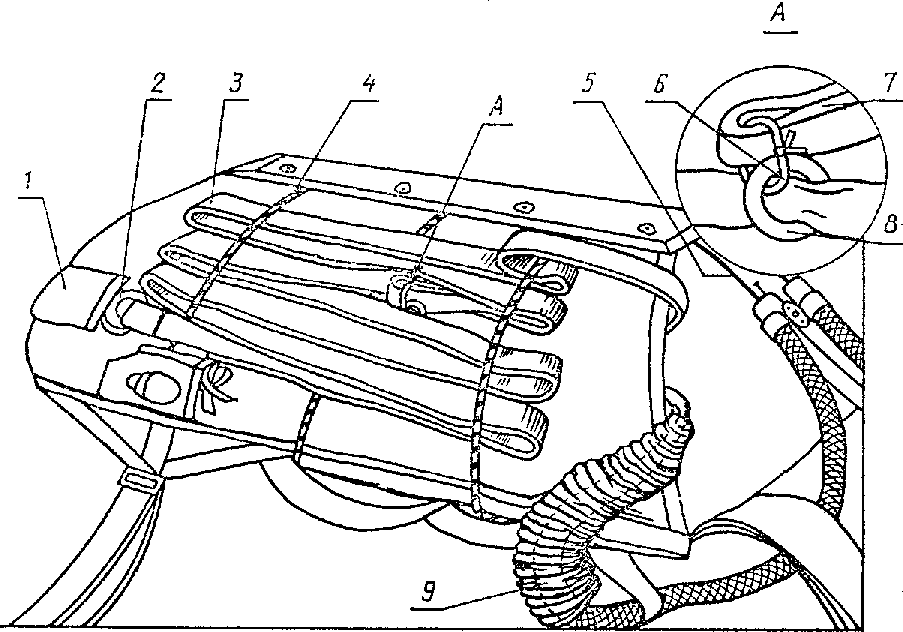
\includegraphics[height=2.8in] {images/38}
	\caption{�������� ��������� ����:}\label{ris38}
	{\scriptsize 1~--- ������; 2~--- �������; 3~--- �������� �������;
	4~--- �������� ������; 5~--- �������� ����; 6~--- ���� ������������
	� ��� ��������; 7~--- �����; 8~--- ������; 9~--- ����������������� �����

	}
    \end{center}
\end{figure}

\subsection{������� �������� �-1-5-� ��� ������ � ������ ����������}

������ � ���������� �������� � ������ � ������ ����������, ������ ������� ��
�������, ������� ������, �������� ������������ ������� ������, ������� ����� �
���� �����, ������� ����� ��������� ��� ��, ��� � ��� ������� ��� ������� �
�������������� ����������� �����.

����� ��� ����� ��������������� ��������� ��������� � ������ �� ������ �������
�������, � � ������������ �� ��������� ������� ����� ��������� ���� �������
���������.

������ ��������� � ������ �� �������� ����� ��������� �������.

\begin{figure}
    \begin{center}
	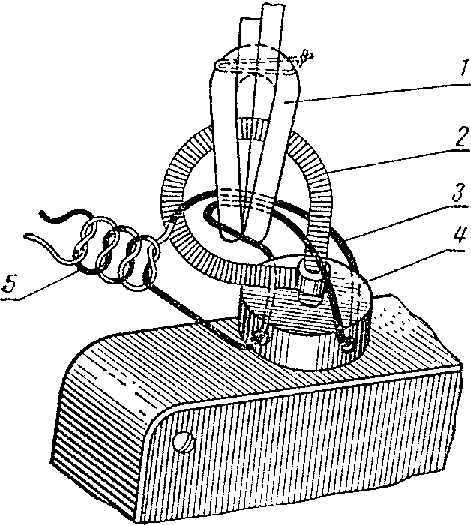
\includegraphics[height=2.6in] {images/39}
	\caption{��������� ������ ������� ������� ���-�:}\label{ris39}
	{\scriptsize 1~--- ���; 2~--- ������ �������; 3~--- ���� ��������;
	4~--- ������; 5~--- ������� ����

	}
    \end{center}
\end{figure}

����� ������� ����� � ��� �������� ���������� ������ ������� ���-� �� �����
��������. ����� ���������� ������� �� ������� ��������� � ���� ������ �������,
�������������� ����������� � ��� ������-������� �������� ���, � ������� ������;
������������� �� ������� �������� ������, ����� ������������ � ������� ������
������� (���.~\ref{ris39}).

\begin{figure}
    \begin{center}
	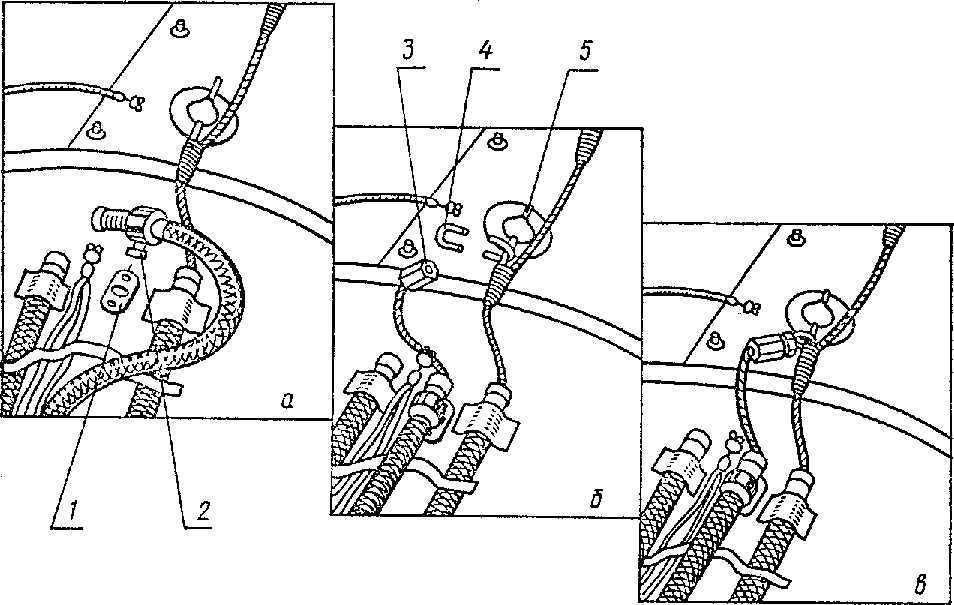
\includegraphics[height=3in] {images/40}
	\caption{������ ������� �� ������� ������ �����:}\label{ris40}
	{\scriptsize �~--- ������������� ������ ������� � �������� �� �����;
	�~--- ������������� ����� ������� � �������;
	�~--- �������������� ���� ���������� ����� � �������;\\
	1~--- ������� �������� �������; 2~--- ���������� ����� �� �������;
	3~--- ����������� �����; 4~--- ����������� ����;
	5~--- ������� ����� ��������� ������

	}
    \end{center}
\end{figure}

����� ������� ������ � ������� ����������� ������ � ��������, �������������� �
������� ������ ����� ����� �������� (���.~\ref{ris40},�). ����� ���������
����������� ������ � ��������� � �������� ������ ����������� ����� �������,
����� ����������� ������ ������� � ������������ ����� ��������� �����.

����� ���������� ����������� ������ ��� ����� �������� ��������� � ��������
��������� ����� ������.

����� ��������� ����������� ������ ��������� ������ � ������� �������� �����
������� ���������. ��� ����� ����������� �� ����������� ����� ���� � ������,
�������� ����� �� ������� �����, ��������� ����� ����� ������ � �������
�������� �����, ������� ����� � ������� ������� (���.~\ref{ris40},�),
��������� � ������� ������������ ����� ����� � ���������� ���� � �����������
����� (���.~\ref{ris40},�). ������� ����� ������� ��� ���� �� ������ ���������
15 ��, � ���� ������� �� ������ ���� �������, ����� ��� ��������� ����������
������� ����� �������������� ����������. ����������� ������� ���������������
�� ���� �������� ������� ������� � ���������� ����� � ���� ��� ������ �������.
����� ��������� ������ ������� ������ ���������� ����� ���� ����� � ������
��������-�������� ��������, ��������� � ������ �� ������ ������� ������� �
������ �������-���������. �������� ��� ���������� ��� �������� �������
(���.~\ref{ris41}).

\begin{figure}
    \begin{center}
	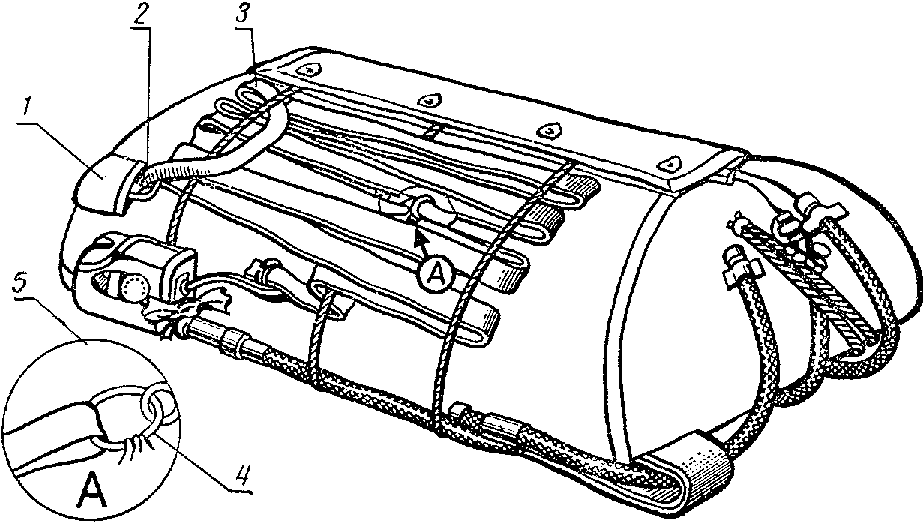
\includegraphics[height=2.5in] {images/41}
	\caption{�������� ��������� ���� ��� ������ ���������:}\label{ris41}
	{\scriptsize 1~--- ������; 2~--- �������; 3~--- �������� �������;
	4~--- ���� ������������ � ��� ��������

	}
    \end{center}
\end{figure}

����� ������ ���������� �������� ��������� ��� ������� � ������� �����������
� �������� �����������, ��������������� ������� ��������.

\section{������� �������� �-5}

{\sc I ����.} {\bf ������ ������ � �������, ���������� �������� � �������.}
������� ����������� � ��������� ������������������: ����� �� ��������,
������������� ��������� �������, �����, ������������ ��������������,
���������� �����.

���������� ������� ���������� ������� �������� �-1-5-�, ��� ������� � ����� II.
��� ������� ����� �������� �-5 ������ �������� ���������� �������� �� ���������
��������� ��������� ���. ����, ������� ���������� � ������� �������, � �������
�� �����������. ����� � ������������� ������, �������� ������ ��� �������.

����� �������� �������� ���� ��� �����������: ������� ���� ��������� ������ �
������ �����; ������ �������� � ������, ������������� �� ������ �������
�������; ����������� ������������� ��������� ������� ���, ����� ������
������� ������-��������� �� �������� 1-� � 24-� ���������� ������.

{\sc II ����.} {\bf ������� ������.} ����� ���������� � ������� ������ � �����
����� ����� ��������� ����� �� ��� �����. ���������, ����� ������ � ������
������ ������ �� ������������. ��������� ������� ��������� ������ ���������
������ �������� ������ �� ��� ����� � ���������, ����� ������ ������� ������
�� ������������ � ������ ������ ������ �� �������� ������ ������. � ������
����������� ����� �� ����� ���������. ����� ����������� ������ (� ������
������ �����, ������ ����� � ������ �������� �����), ������� �� �����,
����������, � ��� ��������� ������ � ��������� ����������� �� ������ ��������
�����. ����� 13-� ������ � �������� �� �� �����������, ���������� ������
������ ������ ����� 12-� � 13-� �������� � ���������� �� ��� ����� ���������
��������� (���.~\ref{ris42},�). ����������� �������� ������� ��� �����
�������� ������ �� ��������� � ��������� ������� � �� ��������� ����� ��������
������� (���.~\ref{ris42},�). ����� ������� ����� �������� ������ ��������
������ ������������� �� �����, ����������� ������ �������� ��-��� ����� �
������� ������ �� 2--3 �� �� ���� ����� � �� ��� ���������� ������ ��������
������, �� 12-� ������ ���������� 11-� ������ � �.\,�. ������ � ���������
������ ������������ ��� ��, ��� � � ����� ��������.

\begin{figure}[!bt]
    \begin{center}
	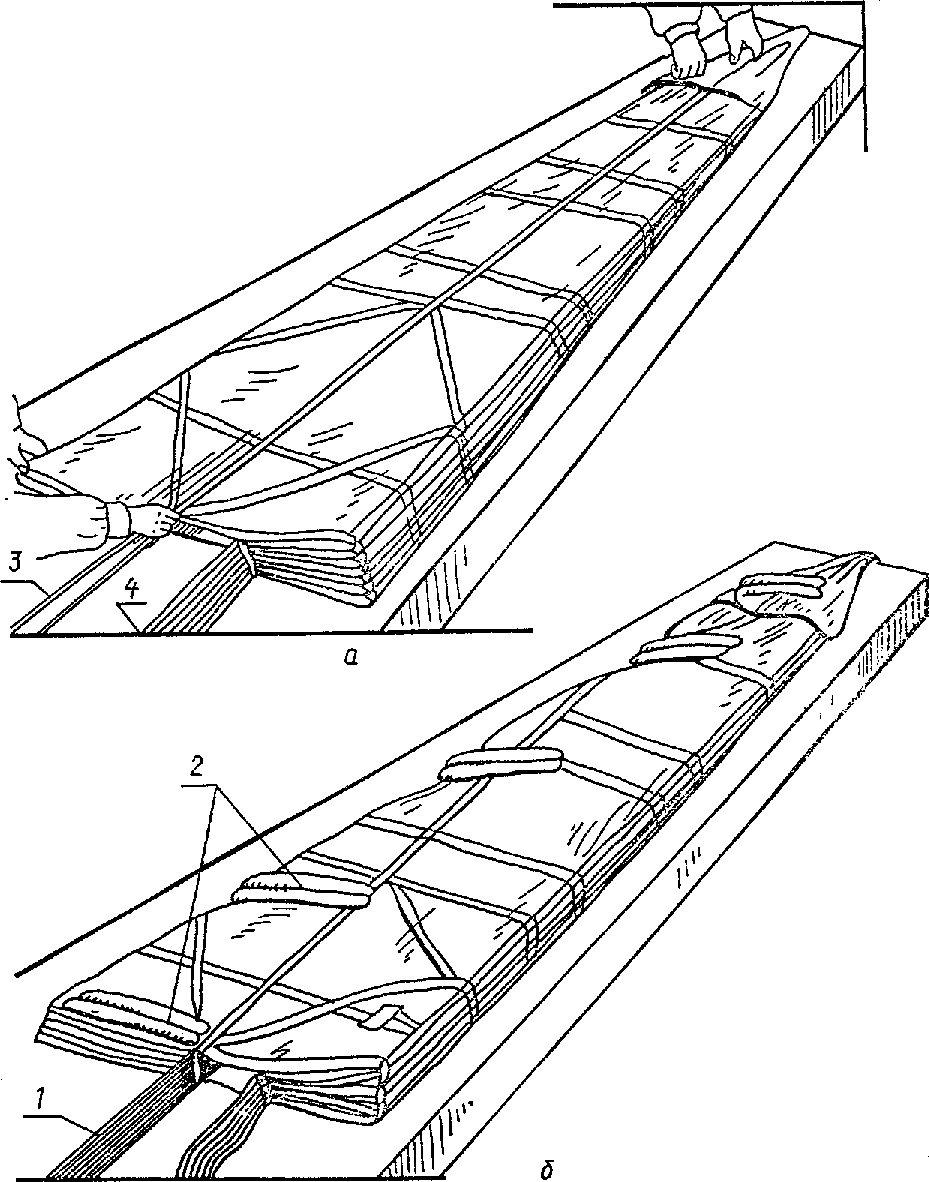
\includegraphics[height=5.2in] {images/42}
	\caption{������� ������ �-5:}\label{ris42}
	{\scriptsize �~--- ������ ������� ���������; �~--- ��������� �������� ������;\\
	1~--- 24-� ������; 2~--- �������; 3~--- 13-� ������; 4~--- 12-� ������

	}
    \end{center}
\end{figure}

����� ��������� ������� �������� ������ ����������� ���� �� ������, �������
������, � ������ �����. �� ����� ����������� �������.

\begin{figure}
    \begin{center}
	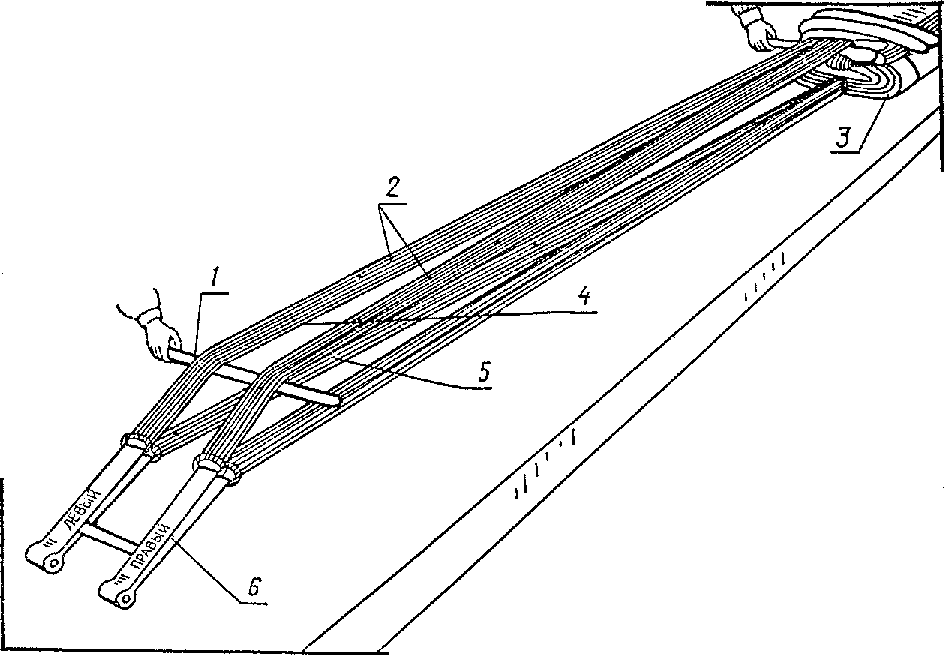
\includegraphics[width=340pt] {images/43}
	\caption{�������� ������������ ������� ������:}\label{ris43}
	{\scriptsize 1~--- ���������� �������; 2~--- ������ �������
	������-��������� ������������� ��������� �������;
	3~--- �����; 4~--- 24-� ������; 5~--- 1-� ������;
	6~--- ������������� ��������� �������

	}
    \end{center}
\end{figure}

������������ ������� ������ ��������� ����� ���������� � ������� ����� �
������ ����� �����. � ������ ������ ������ ����� ������ �� ������ ������������
�� �������� ������ ������. ����� ��� �� �� ������ ������������ � ������ �
����� ������� ������ ������� � ������ ����� (���.~\ref{ris43}).

{\sc III ����.} {\bf ������� ����� � ���� ����� � �������� ������������
������� �����.} ����� �������� �-5 �� �������� � ��������� ��������, �������
�� ��������� ������ � ������� ����� ����� ��������� ��������. ����� ������ ��
���� ������ ������. ������� ������ � �������� ��������� ������ � ������ �������
������ ���������� �����, � ��������� �-5 � �������� �-3~--- ������. �������
������������� ��� �����, � ����� ������������� ��������� ������� ������ ��
����� � ������� ������� �� ���, �� �������� �� ������ ��� �����. ���������,
����������� ����� � ������ ������ �����, ������ ���� � �������� �������.
����� ����� ����� � ������ ����� ����� ���������� ����� ������ � � ����� ����
����� �������� ������� ������ ������. ������� ����� �������� � ����� ����.
�� ����� ���� ������ ��������� � ������ � ��� �������������� �� ������ ���� �
������� �������. ������ ��� ���������� � ���� �� ������ ��������� �� ����� ���
������ ��� �� 3 ��. ������� ����� ����� ��������� � �����, ���������� �� ���.
��������� ����� ����� ����������� ������ �����, ��������� � ����. ���
���������� ������� ������ �� ������ ���� �������� � ����. ����� ���������
������� ������ � ������ ������ ������ ����� �� ������ � ����� ������ � �
����������� ���� �������� � ��������� ����. ���� ������ �� �������� � ����,
�� ������� ��������� ���������.

{\sc IV ����.} {\bf ������� ������ � �����.} ����� �������� ������ �� ���
����� ���������� ������ ��-��� ����� ������� ������ � �������� ��� �������
�������� �� ����� ������������� ��������� �������, �������� �� ��� ����� �����.
�����, ������ �� ��� ����� ������ ������� � �������� �������. �� ������ �����
����� ��������� �� ������. ��� ������ ���������� ������� ����� ����������� ��
������ ����� ������ (���.~\ref{ris44},�). �� ���� ������� ������ ������� � ����
�������. �� ��������� ������� �������� ����� ������ ������ ���� �����������, �
������� ��������� ��������� ������ (���.~\ref{ris44},�). ������������� �������
������ �����������~--- ��� ����� �������� � �������� � ��������� ������ ��� �
������� ��� �����������.

\begin{figure}[!hbt]
    \begin{center}
	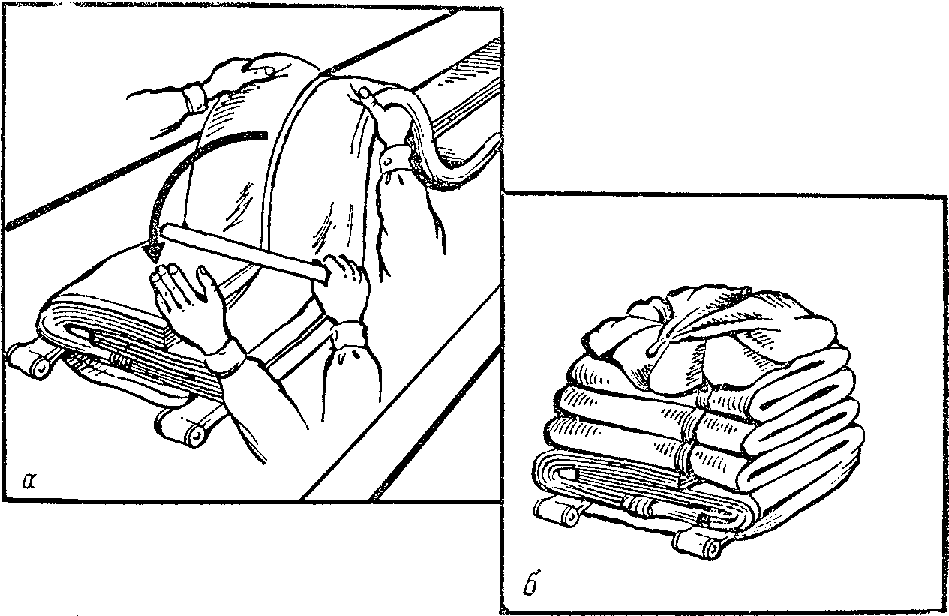
\includegraphics[height=3in] {images/44}
	\caption{������� ������ �� �����:}\label{ris44}
	{\scriptsize �~--- ������ �������; �~--- ����� �������}
    \end{center}
\end{figure}

{\sc V ����.} {\bf ������� �������� �����.} ����� ������� ������ �� ��� �����
��-��� ����� �������� ��� �������.

������� ����� �������� � �������� � ������� �������� � ���������
������������������: ���������� ����� �� �����, ����������� �� ���� � �������
������� ������; ����������� ��� ����� �������� ������� ������, ����� ������
������ � �������� ��� ������ �� ����� �������� �������. � ��������� � ������
��������� ��������������� �������; ��������� ������� � ������ ������� �
�������� �� ����� �������� ������� ������ �������. ��������� ���������������
�������.

����� ������� �������� � ������� �������� ��������� ����� � ����� ����������;
����������� ����� ������� ������ �� ��������� �����, ���������� ������ �
�������� ������-������ �� �����. ������� �� ������-������, ����������� ��
������ ��������������� ������� � ������ ��� ��������� � ����� ������ �������
����� ��������� ������; ����������� ������ ������� ������ �� �����, ����������
������, ����������� ������-������ �� �����, �������� ��������������� ������� �
������ ��� ��������� � ����� ������ ������� ����� ��������� ������.

���������, �� �������� ����� ������, ���������� �������� ��������. ��� ��������
�������� �������� �������� �� ������������ ��������� ������ � ��������.
���������� ����� ������ ��������� ������ ����� �������� � ������� �� ������
��� ������ ���������� �������.

\begin{figure}[!htb]
    \begin{center}
	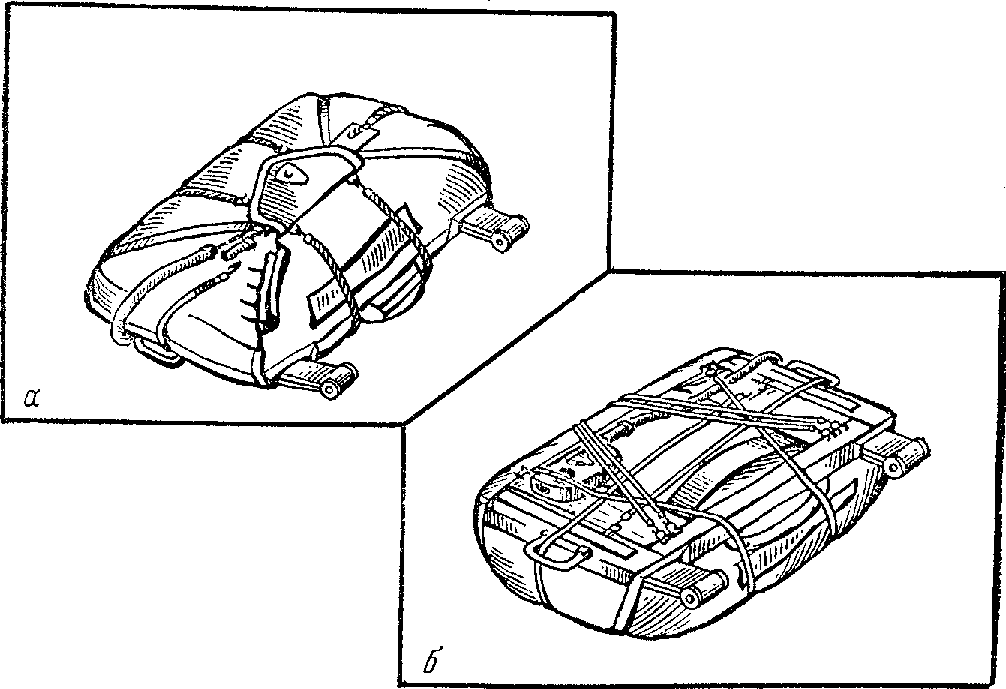
\includegraphics[height=3in] {images/45}
	\caption{������ ������� ���-�:}\label{ris45}
	{\scriptsize �~--- �� ������� �������; �~--- �� ��� �����}
    \end{center}
\end{figure}

����� ������� �� ������� ��������� ������ ���-� (���.~\ref{ris45}), �������
���������� � ����������������� ������ ����������� �� ������-��������.

� �������� �������� ������ ������ � ��� �������. ������ ��������� ���������
������������� � �����������, ������������� �������� �� ������������� �������.

\section{������� �������� ��-15 ����� 5}

{\sc I ����.} {\bf ������ ������ � �������, ���������� �������� � �������.}
������� ����� �������� ����������� � ������������ � ���������, ������ � �����
������� \flqq������� ���������\frqq. ����� �������� ������ ������� ��������
���� ������������� �������������� � �����, ��������� ������������ �������
�������������� ����� � ��������������� �����, ���������, �� �������� �� ������.
��� ����� ����� ����� �� ����� � ������ ��������, � ������ ��������~--- ��
������� � ������. ��� ������������� ������ ���� ���������.

� ������� �� ������ ��������� ������� �������� ��-15 ����� ��������� ����
�������, � ������������ ��������� �� ������������� ������� ������������
���������� ����������.

{\sc II ����.} {\bf ������� ������.} ����� �������� ��-15 ���������� �
��������� ���������. ����� ��������������� ����� � ������� ��������������
����� ������ ������ �� ������� ����������� ����� ��� �����; ��� ������� �
������� �������� ����� ���������� � ������ � ������ ����� ����� �� ������
������ ��������. �������������� ����� ����� ����������.

������� �������� � 12-� ������, �� ������� ����������� 13-� ������. �������
������ �� ���������� ����� ����������� �� ���� (���.~\ref{ris46}) � ����������
���������� ���� ������ � ������ ��� ������. ������ ���������� ������
������������� � ����� 19-� � 6-� �� ������ \flqq������\frqq, ��� ��������������
������ ���������� ������� � ��������� ����� �������� 19-�~-- 18-� � 6-�~-- 7-�.

\begin{figure}[!bh]
    \begin{center}
	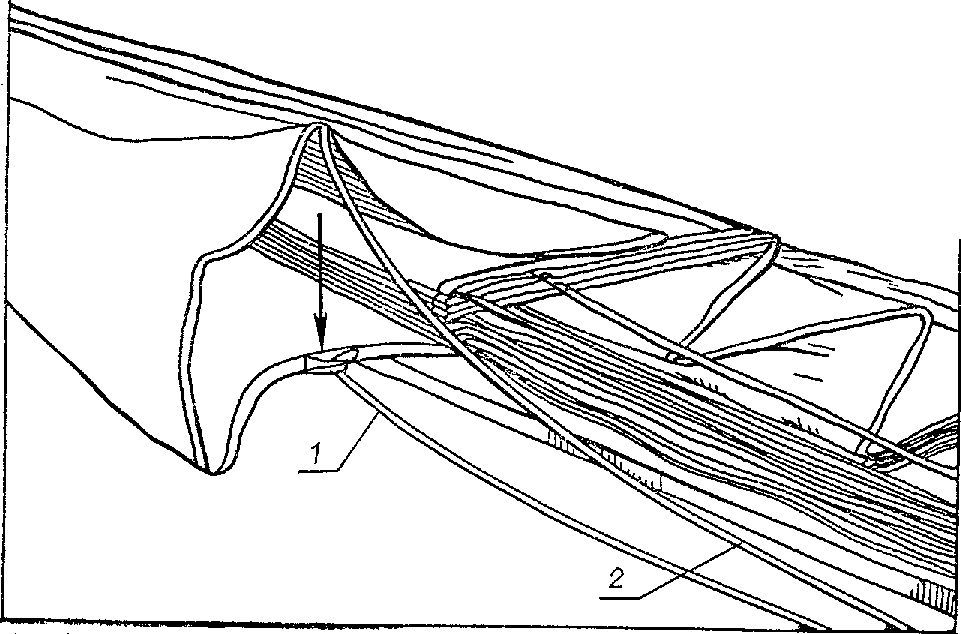
\includegraphics[width=320pt] {images/46}
	\caption{������ ������� ������ �������� ��-15:}\label{ris46}
	{\scriptsize 1~--- 12-� ������; 2~--- 13-� ������}
    \end{center}
\end{figure}

������ ��� ������, ���������� ����������� ������ � ����������� �����������
����� ������, ����������� ������ ������, ��������� �������� �����, �� ���� �
��������� �� 1-�� �� 12-�� ������������� �� ������ ��������. ��������� ������
��� ���� ������ ���� � ������ ��������. ����������� ������ ����������� � ������
�������� �� ��������� ����� ������. ����� ����� 1-� � 24-� ������ � ������
������ � �������� �� ��� �� ������-��������� ��������� �������. �� ����
���������� ��� ������ ������ ���� ������.

��������� ������������ ������� ������ ����� ������� ����� �� ��������� �������
�� ����� � ������ ������ � ������ ������~--- �� ������� � ������. ������ ���
���� �� ������ ���������������. ����������� ������ ��������� �������� ��
�������� �����, ������ �� ����� ������� � �������-����������� ���������
�������, � ������ ���������� ������ ���������� ��� ������ \flqq ������\frqq.
����� �������� ��������� ������ �������� �������� ���������� � ��������������
������ � ����� ������ \flqq �����\frqq{} � ������ �� ���� ����� �������
(���.~\ref{ris47}).

\begin{figure}
    \begin{center}
	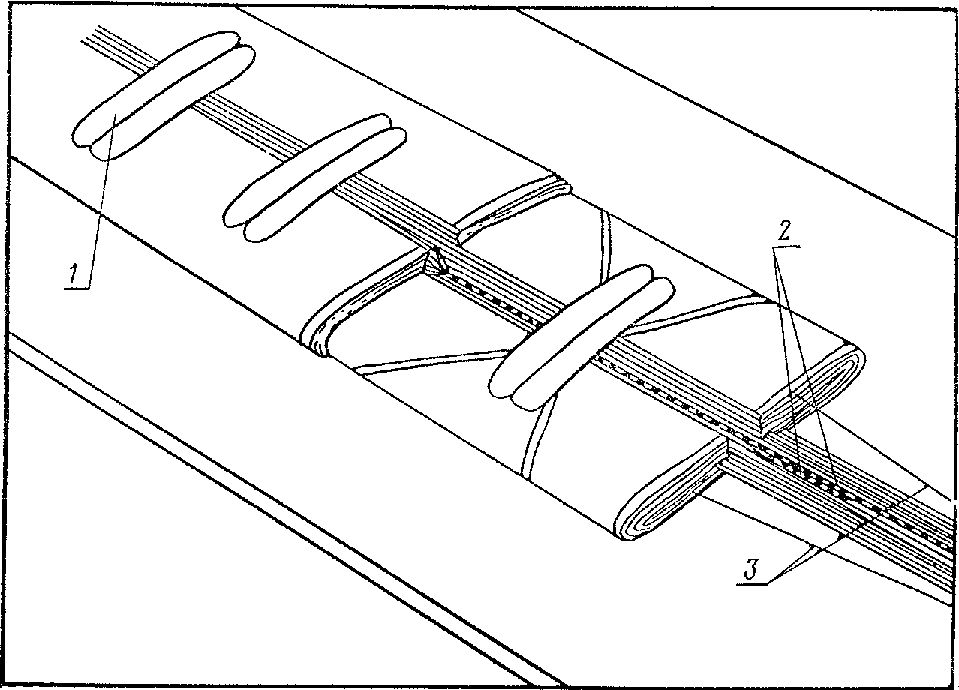
\includegraphics[width=320pt] {images/47}
	\caption{��������� ����� �������� ��-15:}\label{ris47}
	{\scriptsize 1~--- �������; 2~--- ����������� ������;
	3~--- ������ ����������}
    \end{center}
\end{figure}

{\sc III ����.} {\bf ��������� ����� �� ����� � ������� ����� � ���� �����.}
����� ���������� ����� �� ����� ���� ���������� �������������� �����, ��� ���
� ������ ���������� ������ ��� ������ �������������. ����� �� ����� ����������
�� ������ ������ ������. ��� ��������� ����� ������� ���������� �������. �����
����������� ����� ����������� ��� ������ �����, ��������� � ������������ ������
����� ���������� ���� � ����������� ������� �� ��������~--- ������� � ��������
��� ������. �������������� ����� �����������, ��������� ���� �����. ����� ���
������ �� ���������� 0,45 � �� ����� � ������ ������ ������ � ������ �� ��
����� ����� ��������. ��������� �������� ����� ������ ������ ������, � �������
�� ����� ���������� ������� ��������� ����, ���������� � ������ ���� �����
�����, ����� ������������ ������ ����� ����� ����. �� ����� ���� ������
���������� � ������� ������ ����, ����� ��������������~--- � �����, ��
��������� ������ ����� ��������� ����.

��� ������� ����� ���������� �������� �������� �� �������� ������ ����� �����
�� ���~--- ��� �� ������ ��������� 30--40 ��. �� ���� ������� ����� � ����
��������� ������� ����������� � ������. ������� ����� � ���� ����� ������
����������� �� ���������� 1300 �� �� ������-��������� ��������� ������
��������� �������.

����� ��������� ������� ��������� �� ������������, �������� ������ ��
������-��������� �� ��� ������. ������ ��� ���� �� ������ ���������������.
��� �������������� ����� ������� ��������� ������.

����� ������� ����� �������������� ������ ����� ������� � ��������, ��������
���������� ���� � ������, ��������� � ����, ��������� ���������������
(���.~\ref{ris48}). ����� ����� ����� �������� �� �������������� ������ ������
(���.~\ref{ris49}). ����� ��������������� ����� � �������������� ������ � �����
�������� ��������������, ����� ���������� �� ������ ����� � ���������� �
������� ����� ����-�������.

\begin{figure}[hbt]
    \begin{center}
	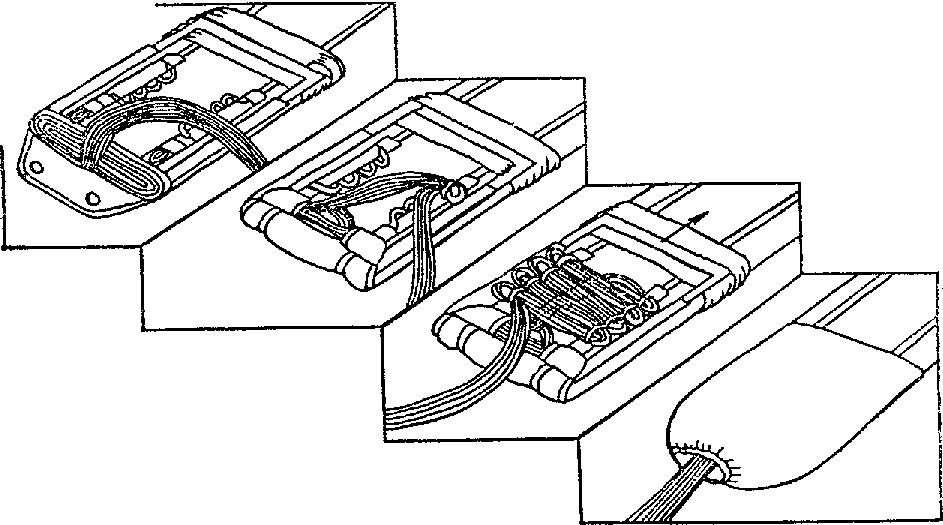
\includegraphics[height=2.5in] {images/48}
	\caption{��������� ������}\label{ris48}
    \end{center}
\end{figure}
\begin{figure}[!ht]
    \begin{center}
	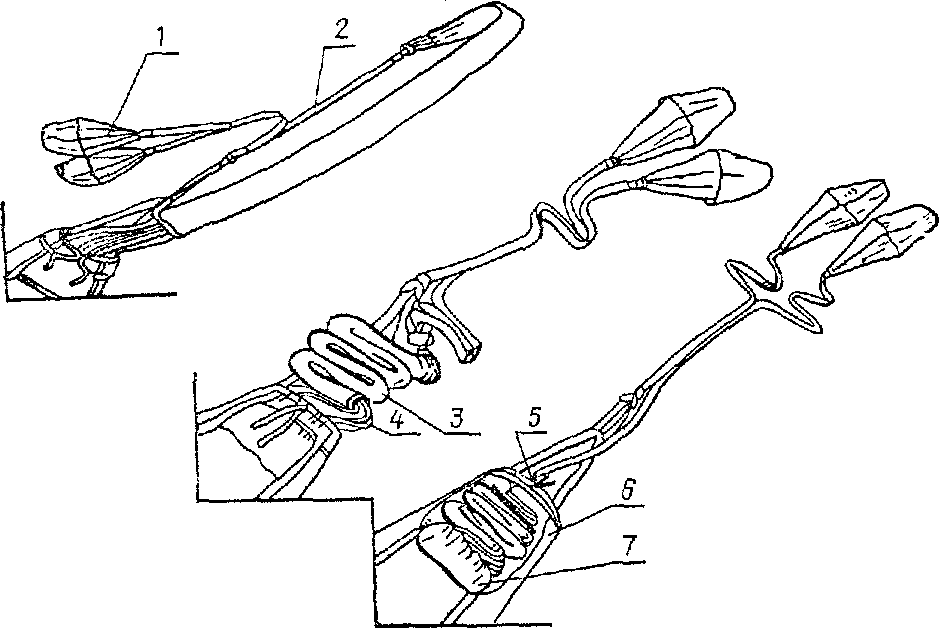
\includegraphics[height=3in] {images/49}
	\caption{������� ��������������� ����� � �����:}\label{ris49}
	{\scriptsize 1~--- �������� ��������; 2~--- ��������������  �����;
	3~--- ����� �������������� �����; 4~--- �������������� ������;
	5~--- �������������� �����; 6~--- ����� ������; 7~--- �����

	}
    \end{center}
\end{figure}

{\sc IV ����.} {\bf ������� ������ � ����� �� �����.} ����� �������� ������ �
����� �� ����� ��������� ����� ��������� ������� ������ �� ��� �����, ��
�������� ��� �����. ������ ���� ������ ����� ��������� ����� � ��������. ���
������� ��������� ������ ���������� �������, ����� �������� �� ������ � ������.

����� ������� ��������� ������ � ����� ������ ������� ��������� ��������� ����
� � ��� ���������� ����� �����. ��� �� �������������� ������ ����. �����
��������� ����� ����� � ����� ������ �� �����, �� �����, ������ ����� ���
�����. ������ ������ ������ ��� ���� ������ ���� �� ���� ��� �� ������� �������
������� �����, � ��������� � ���� ������~--- ������. ���������� ����������� ���
���� ���� ������ � �����. ���� � ����������� ���� �� ������ ��������� ��
�������� �����.

����� ������� ������� ���� ���������� ��� ���� � �������, ��� �������. �����
�����, ������������ ��������� ����, ���������� � ����������������� ��������.
����� ������� ������ ������ � ����� �� ����� ����� ����� � ��������� ����������
������ ���������� �� ������� ������� ������� �����.

{\sc V ����.} {\bf ������� ����� � ������� �������� ���������.}  ������� �����
���������� �� ���� ����������� ����� ��� �� ����������� �������������� �����.

������� ����� ��������� � ��������� ������������������. �� ������� ����� ������
������� �������� ������� ������ ������� �������. � ��������� � ������ ���������
��������������� ������� ��� ������ ������� ��������� �����. ��� ����� ��������
������� ������������ ������ ������ ����. �� ���� ����� ����� ����� ����������
������� ������ ������ �������, ����� ������ ���� �����������, � ����� � �������
�� ���� �������� ������������ �������� ����� ���� � �� ���� ������ �����
����������� ������� ������ ������� �������. � ��������� �� ������ ���������
������ ������� ��������� �����. �������� ��������������� ������� �� �������
������ � ������ ��� ��������� ������� ������� ��������� �����. �������� ����
�������� ������� �� ��������� ���������� ���������, ������� ���, ������������
����� � ������ ������ ��������� �������� ��� ������� � ���������� ��������
������� ��� ������� ����� ����� �������, ����� �������� ��������� ��������
���� ������ � ����� ������� ����������� ��� ������� �������. �������� ������
������ ������� ������� �� ������ ����� ������ ������� � � ��������� � ������
��������� ������ ������� ��������� �����.

\begin{figure}[!th]
    \begin{center}
	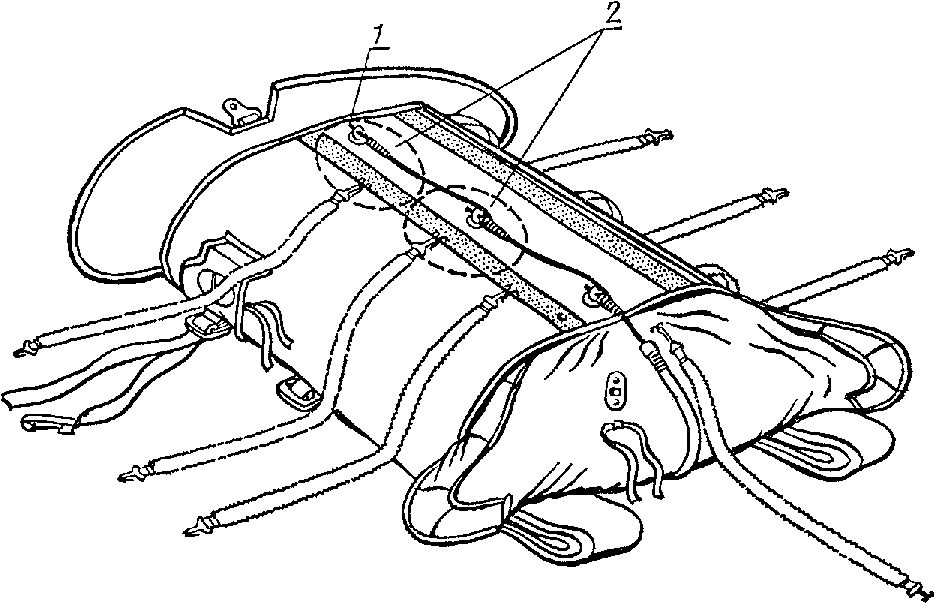
\includegraphics[height=2.7in] {images/50}
	\caption{������������ �������� ��������� � �����:}\label{ris50}
	{\scriptsize 1~--- �����; 2~--- �������� ��������}
    \end{center}
\end{figure}

���������� ������� ������ ������ �������� ������� ��� ������ �����, ��������
�� ����� ������-������ ������� ������� � ������������ ������ ������� �
��������� � ������. ����� ������ ������� � �������� ����� �������� ��������
������ ������������� ���, ��� ��� �������� �� ���.~\ref{ris50}. ��� ��������
�������� ����� ���� ��������� ������������, �� ��������� ����������� ����������
�������� ����� ����� ������ � �������� ���������. ���������� �������� ������ �
������������� �� ������� ���������� ������, ��� ��� ������� � �������
\flqq ������� �������� �-1-5-�\frqq.

\chapter{������������� ������� ������ � ���������}

\section{��������� � �� ��������}

� ������� ��������� �� �������� �� ����������� ���������� ��������� � ���������
�����. ������� ��� ��������� ���������� ������ ��� ���������� ����� ��������
�������� �������, ������� ���� ������� �� ����� ������. ���� �������� ��������
������� � ��������� ������ �������� � ������������, ����� ����� ����������
����� �������� ������ � ��������� �� ���� ������ ���������������.

������������ ��������, ���������� ������ ���, ���������� ���������� (��
��������� atmos~--- ������ � sphaira~--- ���). ��������� ������������ ��
������ ����� 1000 ��. �� ������ ����� �� ����������, ���������������
����������� � ������ �����������, ����������� � ���������. ����������� ���� �
1--2 �� ����� ����������� � ������������ �������� ������ �����������.

���������� ������������ ��� �������� �� ������ 8 ��, ��� ���������~--- 17 �� �
� ������� �������~--- 11 ��. ��� ���������� ���������� ������ ����������
�������� � ����������� ��������� ����������� ������� � ����������� ������.
������� � ����������, ���������� ������� ����������� ������������. ����
����������, � ��� �� ����������~--- ��������������� �� ������� �������
����������~--- ���������� �����������.

� ������ ����� ����������� �� ������ 25 �� ����������� ����������� ���
�������������� ����������� ����������� � ����������� ������. ����� �
����������� ���������, ���������� � ������� ����� ���.

������� � 25 �� � ����������� ����������� ��������� �����������. �� ������
����� 40 �� ��� ���������� ������ $0^\circ$ � � ��������� 40--60${}^\circ$ � ��
������ ����� 60 ��. ���� 60 �� � �� 80 �� ���������� ���� �����������, �������
����� ������������, � ����������� ����� ������ �� ������ 200 ��. � ������
80--85 �� ���������� ���������, ������������ �� ����������� ������� �����������
����������.

�������� ����� �������~--- 75\%~--- ������������� � ���������� � ������������
����� ����� �����~--- 78\% � ���������~--- 21\%. � ������ ������� ������ �����
�����, �������, ���� � �����. ����� �����, ������������ ������, � ���������
������� ���� ��������� ��� ��������: ���� �� ���� ����������, ����� ��������,
�������� �������, ����������� � ������. ���������� �� ����������� � ������� ��
������� ����, ������� ���������, ��������� ���������. ��������, ��� �������
���� ������ ������� ����� ����� ����������� �� ������ �� 2 �� � �����.

{\bf ��������.} ������ ����� ����� � ����� �� ����������� ����� � ������������
�����. ��������� ���������� ����, ������������ �� ������� �����������. ��� ����
������������ ������ $\rho$.

� �������� �������� ������ ���������� � ���/��${}^2$. �������� � 1 ��� �� 1
��${}^2$ ������� �������� ����������� ����������. � ������������ ��������
���������� � �� �������� ������. ��������, ��� �� ������ ����, ��� �����������
���� $15^\circ$ C ������ ����� �� ����������� ����� � ����� 1 ��� �� 1 ��${}^2$.
� ����� �� ����� ����� ����� ����� ������� 760 ��. ����� �������� �������
������� ����������\footnote{ � �������� � ��������� ����� ������������� �������
������ �� �������� ���������� � ��������. 1 �� $=1\frac{\mbox{�}}{\mbox{�}^2}$,
��� �~--- ������~--- ������� ��������� ����.\\
1 �� $=1\frac{\mbox{���}}{\mbox{��}^2}=98100$ ��. 1 �� ��.\,��.~= 133 ��.}.

� ����������� �� ����������� � ��������� ������� �������� ��� ���������, ���,
� ���� �������, �������� ��������� ��������. � �������� �� ������ ��������
���������� � ������ ������������ ��������������. ��� ���� ����������� �������
����������, ����� ��� ����� �� ��� ��� ���� ������.

�������� �������� ���������� � ����������� �� ������ ������������ �
���������-���������� �����������: �����������, �������� ���������������
��������� ��������.

{\bf ��������� �������.} ����� �� ��������, �������� �� �������� �������
����������� � ��������� ����� � �������� ���������������, �.\,�.{} �������� �
��������� ���������, �������� ��������� �������. ��������� �������~--- ���
����� ���, ������������ � ������� ������. ����� ���� ���������� � ��, �
�����~--- � �${}^3$.

������� ����� �����������, ��� 1 �${}^3$. ������� ��� ���������� ��������
(����������� ���� $15^\circ$ C � �������� 760 �� ��.\,��.) ����� �����
1,225 ��, �.\,�.{} ��������� ��� �����
$$
 \rho=1,\!255 \mbox{��/�}^3.
$$

��������� �������~--- �������� ������������. ��� �������� � ����������
����������� � ��������.

���� ��������� ������� � ����������� ����� ����� 1,225 ��/�${}^3$, �� �� ������
6500 � ��� ����� ���������� ����� 0,612 ��/�${}^3$, �.\,�.{} ����� ������. ���
������, ��� 1 �${}^3$ ������� �� ���� ������ �������� ����� ������ ���������.

�� ������� ����� 4000 � ��� ���������� ������� � ��������� ����������
����������� ����������� ����������. ��������� ������� ������ �� ������ ��
�������. �� ��� ������� �������� ������ ��������. ��� ������ ��������� �������,
��� ������ �������� �������� �����������.

{\bf ���������.} ���������� ���������� ���������� ������������� � �������
�������� ����. ���������� ���������� ���������� ���������� ����, ������������
� 1 �${}^3$ �������. ������ ����� ��������� � ���� ������ ������������
���������� �����. ��� ������� �� ���������� �����, ����, ������. �������
��������� ������� ������ ������� �� �����������. � ���������� �����������
������ ����������� ������� ��������� � ���� ������� ����. ��� ��������������
��������� ������� ���������� ������������� ����������, �.\,�.{} ����������
���������� ��������� � ���������� ����, ����������� ������� ��ߣ�� ������� ���
������ �����������.

������������� ��������� ���������� ������������ ���������~--- ������������ �
������������� � ���������� � \%.

���� 1 �${}^3$ ������� �������� 0,012 �� �����, � ��� ��������� ��� ����� ���
������ ����������� ��������� 0,015 ��, �� ������������� ��������� ����� �����
$$
 \frac{0,\!012}{0,\!015}\cdot 100\%=80\%
$$

��� ����������� $+15^\circ$ C ���������� ��������� ��������� 40--60\%.

{\bf �����������.} �������� �������� �����, ����������� ������~--- ������
�����������. ������, ��������� ��������� ����, ����� ����� �� �����������.
��������� ���� ��������� ������ �����������, �� ������� ����������� ������.
��������� ������������� ��������� ���� ����������� ������������ ����� �������.
������������� ��������� ���� ���������� {\it ����������.}

����������� ������� � �������� �� ������ ���������� �������� ����������~--- �
������� �� $0,\!65^\circ$ �� ������ 100 � ������. ����� ����������� � �������
���������� ����� �����, ��� �����. ������������ ������������� �������� �������
�� ��������� ����������� ������� � ��������. ������ ������ �������, ��� �������
��� ����� �������� ����� ������� ������������� ����� ������. ��� �������
���������� {\it ���������} �����������.

{\bf �������� �������.} ���������� ���������� ������� ��������� ������ ���
������������ ����� ������������ ������������. ��� �������� � ��������
����������, ��������, ��� �������� ����������� ��������� ���� � ��� ��� ����
�����������, ���������� ������. ����� ��������������� ���������, � �������
������������ ����� ������� ������������ �����. �������� ����� ���������� � �/�,
� �����������~--- � ��������. ��� ���� ������ ������� �� �����������, ������
���� �����.

�������� �������� ������� ������� �� ������� ���������, ��������� ������� �
�������� ��� �����������. ��� ��������� �������� ���������� ���������� ������
������� ����������� ����� ����� (���������� ��������). ��� ���������� ��������
�������� �������� ������� ����� ��������, ���������� ������������� �����,
���������� � ��������� ������������~--- �������� ���������� ������������.
������� ���������� ��������������~--- ��������� � ������� ��������� ����� ��
�������� � �����������.

��������� ��� ���� �����: �������� � �����������. ��� �������� ���� �����
���������� ����� ������� ������, � ��������� ������ �����������. � �����������
����� �� ������, ��� �� ������. ����� ������� ������ �������� ��� �����
����������.

����������� ����� ������� �� �������� �������� ��� ������������ �����: ��
������ �� ������, ��� � �����������.

����� ��������������� ����������� ������� ����������� � ������������ ���
�����������. ���� ����� ������������ ������ ����� ����������� �������������,
�.\,�.{} ��������� �� ��������� ������� �� ��������� �������. � ������� ���
������ �������� \flqq ���������\frqq.

�������� ������������ ������� � ����������� ����� ������ ���������� 1--2 �/�,
�� � ����� ����������, ����� ������� ������������ ������� �� ����� ������ �
���������. ��� ���������� ������� �������� �������� ���������� ����� ������,
� ��� ���������� ��� �������������. �������� �������� ������������ ������
������ ��� ������� ������� ������� �� ������� 1000--1500 �. � �������� ����
������, ����� ���������, ������� ������� �� ������ 800 �, ���������� ����� ��
������� ������. �������, ������, ��������, ��� ����� ������ ������ ������
����� � ��� ����������� ���������� ����������� � ��� ������ ��������� �������
����� ����������.

������������� �������. �������� � ��������� �����, ���������� ������������
����������, ���� ������������ {\it �������������}.

��� ������� �����, � ������� ������������ ����, ��� ������ ��������������
����� �������������. �������� ������� ������������� ������������� �������~---
�������� �������� ������� � ����� ����������� ����. ����� ����� ���������
���������� ��������, ����� ���� ����������.

������������� ������� ����� ������� � ��������� ����, ��� ������, ����������
�����������. ����, ������� ������� ������, ���������� ������� �������������.
� ������������� ��� ������������� ������, ��� � �������. ����������� ����
���������� ������� �������������, ���, ���� ����� �� ������� � �����, ��
������� ������� ������������ �����������.

������������� ������� ������� �� �������� ��������. ������ ����������
�����������, �������� �� ���� � ��������� ����� ��� ��������� ����� ��������
������������ ����.

����� ����������, ��� � ����������� �������� � ��� ���� �������������
���������� � ������ ����. �����, �������, ������������� ����� ���������������
�������� ��������.

������������� ������� �������� ���� ���������� {\it ������� ��������������
����}. ��� ������ ���������� � �������, ��������������� ����������� ��������
����, � ������������ �� �������
$$
 Q=\frac{\rho V^2}2\cdot C_x S,
$$
\begin{tabbing}
��� \=$C_x$~\=--- \=����������� �������������, ��������� �� ����� ����\kill
��� \>$Q$\>--- ���� �������� �������������, ��� (H);\\
\>$C_x$\>--- ����������� �������������, ��������� �� ����� ����\\
\>\>\>� ��������� ��� �����������;\\
\>$\rho$\>--- ��������� �������, ��� $\cdot$ �${}^2$/�${}^4$ (��/�${}^3$);\\
\>$S$\>--- ���������� ������� ����������� ������� ���� (������), �${}^2$;\\
\>$V$\>--- �������� ��������, �/�.
\end{tabbing}

���� �������� ���� � ��/�, �� ��� �������� � �/� �� ����� ��������� ��
����������� 3,6.

��� ����������� �������� �������� ������������� ���������� ���� ����������
����� ��� ����������� �������������, ������� ������������ ������� �����.
���� ����� ����� �������� � ���������������� ������.

���� ��������� ����� ����� ��������� ������ ��������� � ��������� ������������
�������������. ��������, ��������, ������������ � ������ ���������������, �
������� ���������� ������� ������� ���������. ������� ��������, ���������
������������� �������, �������� �����, ������������ ����� ����. � ������
���������� ������� ��� ����� ���������� ������ �����, � ����� ����������,
���������, ��� ���������� �� ���� �����������.

���� ����������, ��� ��� ������ ����������� �� ����� �������, ��� �������
������������� ���������� ��� ��� �������� � ��������� �����. ��� �����������
���, ��� ������������ ����� ������� �������� ����������� �� ����������� ������.

\medskip
\centerline{\it ����������� ������������� ��������� ���}
\medskip
\noindent������� ��������, ������������� ��� ����� $90^\circ$ � ������ \dotfill 1,28\\
����������, �������� ������, � ������������ � �������\\
������ � ������ \dotfill 0,35\\
����������, �������� � �����������, ��� ����� $45^\circ$ � ��������� \dotfill 0,2\\
��������������� ���������� ������� \dotfill 1,2\\
������� ������� ����� ��� ������������ �������� \dotfill 0,9\\

���� ������� ������������� ����, ����� ���������� �������������, ������������
����� ��� ������� ��� ������� �������� ��� ���������������.

\section{�������� �����������}

{\bf �������� ������� �����������} ������� �� ������� �������, ���������
��������� �����, ������� ��������� ���� � ������������ ��� ��������
�������������.

�� �������� ������� ����� ��������� ���� ������ �������������.

����� ���� ��� ���������� � ������������� ������ � ��������� ����������� ��
���������, ������� �� ��������� ���������, ������� ��������� ��������������
�������� �� ������������ �������� ������� ��� �������� �� �����������.

���� ��������� ������������ �������� ����� ����, �� ����������, ����������
����� �� ��� ��� ���� �������� ��������, ����� �������� ������ �� �����
��������~--- ��������� ���� ������� $g$ � ���������� ���� ����� ���������� ��
�������
$$
 h=\frac{gt^2}2,
$$
��� $t$ - ����� �������, �.

� ����������� �������� �������� � ���� ����� ��� ������ ��������.

�� �������� � ��������� ����� ���� ��������� ��� ����: ���� ������� $G$,
������ ������������ ����, � ���� ������������� ������� ($Q$, ������������ �
�������, ��������������� ����������� ����������� ����. ���� �����������
�������������� ������������ ��������, �� ���� ������������� �������
���������� ������ ���� ������� (���.~\ref{ris51}).

�������� ������� ����� ���������� �� ���� �������, ���� ���� $G$ � $Q$ ��
�������������:
$$
 Q=G=\frac{\rho V^2}2\cdot C_x S.
$$

��� ��������� ���������� �������������� ��������, � ��������������� ���
��������~--- ���������� (�����������) ���������.

����������� �������� ������������ �� �������
$$
 V_{\idx{��}}=\sqrt{\frac{2G}{\rho\cdot C_x\cdot S}}.
$$

��� �������� ��� $C_x$ ����������� 0,3 ����� ����� 42 �/�, � ��� $C_x$
����������� 0,15~--- 58 �/�.

��������� ��������� ������� � ������� ��������, �� � �������� ������� �����
��������� ��������.

\begin{figure}
    \begin{center}
	\includegraphics[height=1.5in] {images/51}
	\caption{��������������� ��� ��� ������� �����������}\label{ris51}
    \end{center}
\end{figure}

����������, ���������� ������������ �� ����� ������� � ������ 1500--2000 � �
����������� �� ��������� ����, �������� � ����.~1.
\begin{table}
    \flushright{\it ������� 1}\\
    \begin{tabular}{c|c|c|c}
    \hline
    & \multicolumn{3}{|c}{��������� ����}\\
    \cline{2-4}
    ����� �������, & ����������   & ������������ & ����������\\
    �		   & ���� ������� &		 & ������\\
    \cline{2-4}
    & \multicolumn{3}{|c}{����������, ���������� �����, �}\\
    \hline
	1 &	4,9 &	4,9 &	4,9\\
	2 &	19,5 &	19,5 &	19,5\\
	3 &	44,0 &	43,8 &	43,5\\
	4 &	76,0 &	75,0 &	73,5\\
	5 &	114 &	110 &	105\\
	6 &	160 &	150 &	140\\
	7 &	210 &	193 &	178\\
	8 &	262 &	240 &	218\\
	9 &	318 &	287 &	255\\
	10 &	375 &	335 &	300\\
	11 &	430 &	380 &	342\\
	12 &	488 &	430 &	384\\
	13 &	546 &	480 &	426\\
	14 &	601 &	530 &	468\\
	15 &	660 &	580 &	510\\
	16 &	718 &	630 &	552\\
	17 &	776 &	680 &	594\\
	18 &	834 &	730 &	636\\
	19 &	892 &	780 &	678\\
	20 &	950 &	830 &	720\\
	21 &	1008 &	880 &	762\\
	22 &	1066 &	930 &	804\\
	23 &	1124 &	980 &	846\\
	24 &	1182 &	1030 &	888\\
	25 &	1240 &	1080 &	930\\
	26 &	1298 &	1130 &	972\\
	27 &	1356 &	1180 &	1014\\
	28 &	1414 &	1230 &	1056\\
	29 &	1470 &	1280 &	1098\\
	30 &	1530 &	1330 &	1140
    \end{tabular}
\end{table}

� ����������� ����� ����������� ������������� � �������� ��� �������. ���
����, ������, ���� ���������, ��� ���������� ����� ����������� ������ �������
� ����������� ������ ����, � �������������, � � ����������� �������������
�������, ��� � ������� �������� � ��������������� ���������� ��������.
�������������� ����� �������, ��� ��������� ����� ����������� �� 10 ��
�������� ��������� �������� ��� �������������� ������� �� 2\%, ��� �
����������� ����� �������� ������� � 1 �/�.

{\bf �������� ��� ��������� ��������.} ��� �������� �������� � ��������
���������� �������� ������������� ��� ������� ��������. �� �������� ��������,
��� ������ ��������� �������� � ������� ������� �� �������� ��� �����������
���������� ����������.

����, ��������, �������� � ������ �������� ���� $V_1$, � ����� ����� $t$ �����
$V_2$, �� ������� ��������� ���������� �� �������
$$
 a=\frac{V_2-V_1}t,
$$
\begin{tabbing}
��� \=$V_2$~\=--- ���������;\kill
��� \>$a$\>--- ���������;\\
\>$V_1$\>--- �������� � ������ ��������;\\
\>$V_2$\>--- �������� � ����� ��������;\\
\>$t$\>--- �����, �� ������� ��������� ��������� ��������.
\end{tabbing}

���� �������� � ������ � ����� ��������, �������� ��� ��������� ��������, �
����� �����, �� ������� ���������� ��� ������ ���������, ����� ����������
�������� �������� ���������.

���� ������� �������� ������� $V_1$, ������ 50 �/�, �������� ����� ���������
�������� $V_2$, ������ 5 �/�, � ����� $t$, �� ������� ��������� ������
��������� ��������, ������ 2 �, �� �������
$$
 a=\frac{V_2-V_1}t=\frac{5-50}2=-22,\!5~\mbox{�/�}^2
$$

���� ����� ��������� �� ���������� (����������) �������� �������.

����, ��� ��������� ��� ��������� ������� ����� 9,81 �/�${}^2$, ���������, ��
������� ��� ����������� ���������, �.\,�.{} ������ �������� ����������:
$$
 n=\frac ag=\frac{22,\!5}{9,\!81}\approx 2,\!3.
$$

���� ������ � ����������, ����� ���������� � �������� $F$, ����������� �� ����
� ������ ��������� ��������. �� ��������� �� �������
$$
 F=mgn.
$$

��� ����� ����������� 70 �� �������
$$
 F=70\cdot 9,\!81\cdot 2,\!3 = 1579,\!4~\mbox{� (161 ���)}.
$$ 

��� ������, ��� ���������� � ������ ��������� �������� ��� ��
\flqq����������\frqq{} � ����� �� ��������, ���������������� ����������. �����
���������� ������� ��������� �����, ��� ����� ��� ��� ��������� �� ���������,
� ��������� ������������ �������� ����� 2 �, �� ������� ���������� ���������
��������.

{\bf �������� �������� � ��������� ���������.} ��� �������������� ��������
�������� � ���������, �� ������� ����������� �������������� ��������, ����
������������� ������ $Q$ ��������� � ���������� � ����� ������� $G$. ���� �
���� ������ �������������, ��� ��� ������� �� ���.~\ref{ris51}.

����� ���������� ����������, �.\,�.{} $G=Q$, �����
$$
 Q_{\idx{����}}=\frac{\rho V^2_{\idx{����}}}2\cdot C_x S.
$$

���� $V_{\idx{��}}=V_{\idx{����}}$, ��
$$
 G_{\idx{����}}=\frac{\rho V^2_{\idx{��}}}2\cdot C_x S.
$$

������ �������� �������� � ����� ��� ���������� ������� �����
$$
 V_{\idx{��}}=\sqrt{\frac{2G}{\rho\cdot C_x\cdot S}}.
$$

���� ������� ���� ������� ������� $G=90$ ���, ����������� ��������
������������� $C_x=0,9$, � ������� ������ �������� $S=55$ �${}^2$, �� �������
$$
 V_{\idx{��}}=\sqrt{\frac{2G}{\rho\cdot C_x\cdot S}}
 =\sqrt{\frac{2\cdot 90}{0,\!125\cdot 0,\!9\cdot 55}}
 =\sqrt{\frac{180}{6,\!1}}=\sqrt{29,\!5}=5,\!4~\mbox{�/�},
$$
��� ������������� �������� � ������� �������� ��-15.

����������� ���������� �������� ����� ����������� �������������� ��������.
��� ���� �� ����������� ������������ ��� �������� �� ������ ������ � ���������
������ �� ��������� � �����, �� � ������������ ��������� ����� � ��� ��� ����
�����������. ����������� �������������� �������� ��������� ������� �� ����
����������� �������, ����������� ��� ������ ������� ����� ��������� � ������.

�� ������������ ��������, ��� � ���������� ����������� ���� � ��������� �����,
����, ����������� �� ����, �� ��� �����������, ���������������� ����
������������� �������. ��� ������� ��������� ���� ��� �������� �� ���
����������� ����� �����������. ��� ���������� ����� �� ��� ���������
�������������� ����, ������������ ��������������� ����� ��������.
� ������������ ��� ���� ���������� ��������� � ������������ ������ $Y$.

���� ��� �������� � ������� ����� �����, ��� �������� ��� ������ ��������,
��� �� �����, �� ��������� ������������ ������� �� �������� �������� ���
������� � ���������, ������� ����������� �������������� �������� �����������,
� � ��� ���������� ���������.

���������� ����� ���������� ��� ��� �������� � ����� ������� (���.~\ref{ris52}).
\begin{figure}
    \begin{center}
	\includegraphics[height=2.8in] {images/52}
	\caption{����� ���������� ��� ��� ��������������� � ����������� �������}\label{ris52}
	{\scriptsize $G$~--- ����� �������� ��� ������� \flqq ���������� + �������\frqq;
	$Q$~--- ���� �������� �������������; $Y$~--- ��������� ����;
	$W$~--- �������� ���������������; $R$~--- �������������� ����

	}
    \end{center}
\end{figure}
%    \vbox{\centerline{\scriptsize $G$~--- ����� �������� ��� ������� \flqq ���������� + �������\frqq;
%	$Q$~--- ���� �������� �������������; $Y$~--- ��������� ����;
%	$W$~--- �������� ���������������; $R$~--- �������������� ����}}

� ���������� � ���������� ������� ����������� �������������� ��������
���������, ��� ����������� ����, ��������� ���� $Y$, �������� ������� �������
�� ���� ������������� �������, ����������� � ����������� ��������.

��������� �� ���.~\ref{ris52} ���� $Q$ � $Y$ ����� ����� ����� � ������������
�� �������
$$
 Q=Y=\frac{\rho V^2}2\cdot C_x S,
$$
� ������� ����������� $C_x$ � ������� $S$ ������� �� ������ ������� ������� �
�������� �� ��������� ��������.

����������, ��� ������ ��������� ���� �� ���������������, � ����������
��������������� ����������.

��� �������������� ��������, ��� �� ���������� ����, ������� ��� $G=90$ ���
����� ��������� �� ��������� 5,4 �/�.

��� ����������� ����, ����������� �� ���������� �������, �������������� �
�������������� ����������� (������� ��-15 � �������� ������), ����������
���������� �������� $Y$ � $Q$ � ����� �� �������������� $R_{QY}$, ��� ���
������ ��� �������������� ���������������� ���� ������� $G$. ��� �����������
�������� �������� �������� ���������� ������� ������� ��������� ������:
$V_{\idx{���}}=5$ �/� (����� ��-15 ��� �������� � �������� ������), $C_x$
������ $\approx 1,\!2$, � $S\approx 35$ �${}^2$.

��������� �� ���� ������ $Q_1$.
$$
 Q_1=\frac{\rho V^2}2\cdot C_x S =\frac{0,\!125\cdot 25}2\cdot 1,\!2\cdot 30=54~\mbox{���}.
$$

���� $Q=Y$, �� � $Y=54$ ���.

��� ��������, �������������� ���� ���������������� ��� �����
$$
 R_{QY}=\sqrt{Q^2+Y^2};\quad R=\sqrt{54^2+54^2}=\sqrt{5832}\approx 76~\mbox{���}.
$$

�������������, ���������� ������� ����� ��� �� \flqq �����\frqq{} �� ���
��������. ���������� ���������� �������� � ������� �������� ��������,
��������� �������� �������� �������� �������
$$
 V_{\idx{��}}=\sqrt{\frac{2G-R_{QY}}{C_xS\rho}}
 =\sqrt{\frac{180-76}{1,\!2\cdot 55\cdot 0,\!125}}
 =\sqrt\frac{104}6=\sqrt{17,\!3}=4,\!2~\mbox{�/�}.
$$

��� ��� ������� �������� $Q$ (���� ����� �������� ����������, ��������, ������
�����, ������� �� ��������� 8 �/�), ������ ��������� ���� ����� �����
������������~--- ������������ �������� �������� �������� ����� 3--3,5 �/�.
���� ����� �������� ���������� � ������, ���������� �� ��������� ����� 12 �/�,
�� ���������� ������ ����������� �����.

����������� �� ���� ������� �������� ������ ��-15 ��� �������������� ��������
����� ���������. ��������, �� ���� ������������� ��������� ������ ����� ��
������������. ������� ������ ���������������� ����� ����������� ��������������
�������� �� 6,5 �/�.

\section{����������� �����������}

�����������~--- �������� �������������, ����������� ���� ������. �������
������ ������������� ��������, ��������� � ������������, ������ ���������
��� ������ �� �������� �������� ������� �������� ����������� �����
�����������, ������� ����������� ���������� ������ ��� �����-����
�������������� �����������. ����������� ��� ������ � ��������� ���������� �
������������ ���������, ������� ������������ �� �������� �������� � ��������
��������������� �����������. �������������� ����� ���� ��������� ����������
{\it ��������� �����������} (���.~\ref{ris53}).

\begin{figure}
    \begin{center}
	\includegraphics[height=3.4in] {images/53}
	\caption{������ ��������� ��� ����������� �����������}\label{ris53}
    \end{center}
\end{figure}

������������� ��� �������� ���������� ��������
$$
 W_{\idx{��}}=\sqrt{V^2_{\idx{�}}+V^2_{\idx{�}}},
$$
��� $W_{\idx{��}}$~--- �������� �����������;\\
\mbox{\qquad}$V_{\idx{�}}$~--- ������������ �������� ��������;\\
\mbox{\qquad}$V_{\idx{�}}$~--- �������������� �������� ��������.

���� ���������� ��������, ��������������� ����������� ����������� � ���������
�-1-5-� (����� ������� 100 ��), ��� �������� ����� $U=2,\!5$ �/�, �� �������
$V_{\idx{�}}+U=2,\!5+2,\!5=5$ �/�.
$$
 W_{\idx{��}}=\sqrt{V^2_{\idx{�}}+V^2_{\idx{�}}}
 =\sqrt{4,\!25^2+5^2}=\sqrt{43,\!06}\approx 6,\!5~\mbox{�/�}.
$$

��� ���� �� �������� ��� �������� ��-15 �������� ����������� ������� ������,
��� ��� $V_{\idx{�}}$ ������� ��� ����� 100 �� ����� 4,5 �/�, � $V_{\idx{�}}$
��� ������� ������ � ����� 2,5 �/�~--- 7,5 �/�. �������� ����������� � ����
������
$$
  W_{\idx{��}}=\sqrt{4,\!5^2+7,\!5^2}=\sqrt{76,\!5}\approx 8,\!8~\mbox{�/�}.
$$

����������� � ����� ��������� ������� ����������� ����������, �����������
����������� ��������� ����������� ��� ����������� ��������.

����� ������� ��������� ����������� ����� �������� ������� �� ���������, � ��
�����-�� ������� ����, �� ������� ���������� �������� ���� ����������� �
������ ��������. ���� ���� ������� ������� ������ 1 �����.

��������, ������������ ������������ ��� �����������, ���������� �� �������
$$
 F=\frac{m\cdot W^2_{\idx{��}}}{2i}.
$$

���� $i$ ����� 1 � (������� �������� ���� �� ������ ������� ����������� ��
�����), � $W=7,\!1$ �/� (�������� ����������� ��� ������� �����), ��
$$
 F=\frac{m\cdot W^2_{\idx{��}}}{2i}
 =\frac{90\cdot 7,\!1^2}{2\cdot 1}\approx 2268,\!45~\mbox{� (231,2 ���)},
$$
���������� ��� ���� ��������
$$ 
 n=\frac{F}P=\frac{231,\!2}{90}\approx 2,\!57.
$$

��� ���������� �������� $W$ �� 9 �/� (��� ������ ����������� � ��������� ��-15
��� ������������ �����) ������� ��������
$$
 F=\frac{m\cdot W^2_{\idx{��}}}{2i}=\frac{90\cdot 9^2}2
 =3645~\mbox{� (372,5 ���)},
$$
��� ������������� ����������
$$ 
 n=\frac{F}P=\frac{372,\!5}{90}\approx 4,\!14.
$$

����� ���������� ����������������~--- ��� ����������� ��� �����-����
�������������� ��������� � ���������.

� ������� ����������� ����������, �������������� ��� �������� ����������,
����� ����, �� ������� ���������� ����������, ����� ���������. ��������,
���������� ������� \flqq �������\frqq{} ��� ����������� ��������� �����������
��������� ����, �� ������� ���������� �������� ��������, ��� �����������
�������� �������� ��� �����������.

��� ������� ������� �������� ����������� � ��������� ��-15 ��� ����� 5 �/�, ��
\flqq �������\frqq{} � \flqq �����\frqq{} ������. ��� �� ����������, ��������
�������� ���������� ������� ��-15 � �������� ������ ��� ����� 90 �� ��
\flqq �����\frqq{} ����� ����������. 4,2 �/�. �������� � ���� ������ �����
$$
 F=\frac{m\cdot W^2}2=\frac{90\cdot 4,\!2^2}2=793,\!8~\mbox{� (81 ���)}.
$$

��� ����������� �� \flqq �������\frqq{} ����� �������� ����������� ���������,
��� ���
$$
 V_{\idx{�}}=V_{\idx{�}}+U=5+5=10~\mbox{�/�},
$$
$$
 W_{\idx{��}}=\sqrt{V^2_{\idx{�}}+V^2_{\idx{�}}}
 =\sqrt{100+17,\!6}=\sqrt{117}\approx 10,8~\mbox{�/�},
$$
��� ���� ��������
$$
 F=\frac{m\cdot W^2}{2i}=\frac{90\cdot 10,\!8^2}2=52665~\mbox{� (536 ���)}.
$$

����������� � ������ ���������� ��������� ������ �� ������ ��������������
�������� (���� � ������������� ������ ��������� �� ����� ��� ������ �������
����������) ��� ��������������� ���������� ������������ � �����������.

����� �� �������� ���������� �������� � �������, �� ��������� � �������
��������� �����������, �������� ���������� �������� ����������� �� ����
�������� ������ ����� ������������ �� \flqq �����\frqq{} ����, ��� �������
�������� ����������� ��� �������� ������������� �������� ����� ������� ��
�����������.

��� ���������� ������������� �������� � ����������� � ��� ��� ���� ���������
����� ������� ������ ���������, � �������� ��������� ����� ����������
����������� �������� �����������.

���� ���������� �������������� �������, �� ������ ������ ��� ���������� ������
�������� ����������� ����� ���������� �� ����.~2.

{\flushright{\it ������� 2}\\
\begin{tabular}{c|c|c|c|c|c|c|c}
    \hline
    �������� �����������, �/� &   3  &   5 &   6  &   7  &   8  &   9  &   10\\
    \hline
    ������ ������, �	      & 0,46 & 1,27& 1,83 & 2,50 & 3,26 & 4,12 & 5,10
\end{tabular}
}
\chapter{�������� ��������� ��������� ������ � ���������}

\section{���������-������������� �������}

����� ������ ������ � ��������� ��� � ��������� ������ ��������, ��� � ���
������� ������������� ����� ��������� ������� �� ���������������� �����������
� ���������� ������� ������.

������������� � ������ ����� ������ �� �����, �� �������� �������������
����������. ����� ������� ��������� ������ ���������� �� ����������� ���
��������~--- �� ��������� �������� �� �����������. �� ������������� �����
������ ������ ��� ��� ��������.

����������� ����������� �� ��������� ��������� ������ � ��������� �
����������� ���������� �������, � �������� ������������ �������� ������
��������� ��� ���������:\\
\mbox{\quad}������ ������� � �������, �������� ������, ���������� � ��������
��� ���������� �������, ���������� �������� ���������� � ������������ ��
�������� �����������, ��������� ������� ��������� �� ��������;\\
\mbox{\quad}���������������� � ������� � �������� ������������ ��� ���������;\\
\mbox{\quad}��������� ���������� ������� ��� ��������������� � �����������;\\
\mbox{\quad}�������� ��� ��������� ��������� ��������;\\
\mbox{\quad}��������� �����������.

� ����� ������� ����������� �������� ��� ��������� ���� ��������
�����������~--- �� ��������� �� �������� �� �����������.

��� ��� ��������� ����������� ��� ��������� ���������� ������������. �� ����
������������ ����� � ������� ������������� � ����������� ����������
����������� ��������.

��� ���������� ������� ������������ �� ���������� ���� �� ����������
������������ ������������ �������������� ���������. ��� ����� ��� ���������
����� ���������, ��� ���������� ����� � ��������� �������, ����������� �������
��� � ��������� ����������, ��������� �������� �����������.

����� ��� ����������� �������������� ������� ������� �� ���.~\ref{ris54}.
\begin{figure}
    \begin{center}
	\includegraphics[width=340pt] {images/54}
	\caption{����� ����������� �������������� �������:}\label{ris54}
	{\scriptsize 1~--- ������� �����; 2~--- ����� �������� ��-2;
	3~--- ������� � ���������� ���������; 4~--- ��������������� ��������;
	5~--- �����; 6~--- �������������� ������; 7~--- ������;
	8~--- �������� �����; 9~--- �������� �� ��������� ��������
	������������ ��� ���������; 10~--- ������ �� ������;
	11~--- �������� �� ��������� �������� ��� ������� ������;
	12~--- �������� �� ��������� �������� ��� ���������� ����� �
	��������� �������

	}
    \end{center}
\end{figure}

���������� ���������� ������������ �� �������� ��������� ��������� ������ ���
���������� ������������ ����������������� 20 �����, ���
�����������-������������~--- 30 ����� � ��� �����\-���\-���-��\-��\-��\-��\-����,
���������� ���������� ���������� �����������������,~--- 20 �����.

�������� ���������� ���������� � �������� ������� �� ���������� ��������,
������� � �������� ���������� ���������� ������� ��� ���������� ������.

{\bf �������� ��������� �������, ������ ��������� �������� � ���������
��������.}

��� ����������� ����������� �������� ��������� ����������� � ���������
���������� �� ��������� �������. ����� ����, ���������� �� ������ ������������
�������� ��������� ��������, � ��� ������������� �����-���� ��������������
��������� ���������� ����������� ��� �������� �� �������� � ������ ���������
��������.

������ ����������� ������ ��������� � ������������ ���������� �������, � �����
��������� ������������ �� �������� � ������� ����������� �������� ����������
����������� � ���������� ���� ������������� ��� �������.

� �������� ����������� �� ������� ���������. � �������� ���������� ���������
�������� ������� ���������� ��������� �������, �������������� ������ � ����
��� ����������� �� �� �����, ����������� ������ � ���������� ����� � ������,
��� ������� ������������ ������������� �����.

������ ����� ����������� ����� �� ��������� ��������, ���������� ��������� �
�������� ��������, �������� �� ����������.

� ������ ���������� �������� ������� �������� ��� ��������: ���������� �
����������. ���������� ����� ������� ������ ����� �� ����� �����, ������������
��� � ����������� ����� ���� � ��������-�������� ������. ���������� � ���
����� ������������ ������ ����� �, ����������� ������� �� ������ ����� �����,
�������� ��������� ����������� ������ ���� � ������ ��������-�������� ������.
������� ��������� � ������ ������� ����������� ���������� ����������.

����� �������, ���������� �������� �����, � ����� ��������-��������, ������ �
������� �������.

�� ���������, �� ������� �� ��������� ������� ������ ���, �������� �����
���������� ��������� ������������� ������ ����� ��� ����.

��� ��������� ���������������� �� ����� ��������� ������� ������������� ������
������������� �� ������ ������, � �������� ����� � ������ ����� ��������� �
���� �����������, �� ������� ��� � �� ���� ������ �������. �������� ���������
���� � ����.

��������-�������� ������� ���������� �� ���� ����������� �� � �������������
������� � ������ �������. �������� ������� � ������ ������� ��������� �������
� ������� ������.

�� ���������, ������� �� ��������� ������� ����� ���, �������� �����
���������� ��� ������ ��������� ������, ������������� �� ���.

��������-�������� ������� ������� ��������� ���, ����� ������� ����� ��������
�������� ������������ �� ������ ���� �����������. ��� ������� ����������
�������������� �� ��� ��������.

������ ������� ���������� �������������� �� ��� ��������. ��� ����������
�������� ��� ������� �������� ������ ��������� � ���� �������� �����������.
� ��������� ����������� ���� ������ ������� ����� ��������� �������.

������� ������ ���������� ����� �������������� �� ��� ��������. ���������
���������������� ������� ������ �� ������ ������� ������ ��������� �
����������� � � �� �� ����� �� ������ ���������.

�� ���������, �� ������� �� ��������� ������� ������ ���, ����������� ��������
������� ������������ �������� ������������ ������� ���������. �� ���������,
������� �� ��������� ������� ����� ���, ������� ��������� ������������
������������� �� ��� �������.

��������� ����������� ��������� ������� �� �������� �������� �����������,
������ �������� ����, �� ��������� ���������� �� ����������� ����� � ��������
� ������������ ����������� ������������� �������� �� �����������.

������������ �������� ��������� ����������.

�������� ��� ��� ���� ��� ��������, ��������� ������ ���������
����������������� �������������� ������ � ��� �������� ���������� �������� ��
��� ��������� ���������� ������ ���, ��� ��� ������������� �� ����������
��������.

������� �������� �������� ��������� ���������, ���� ���������� ������ �
�������� �������� �� ������ ���� ������� �� ��� ���������.

������ �������� ��������� ��������, ������� ��������� ��������� �����������
�������� �������.

� ���������, �� ������� �� ��������� ������� ������ ���, �������� �������
������������ ��� ������ �������� ���������. ��� ����������� ���������� ������
� ����� ���������� ����� ������������� ��������� �������. ����� ���������
��������� �� ������, �������������� � ��������� ������� ��������� ��������,
����������� � ��������� ��������� � ����� � ������� ����������.

� ���������, ������� �� ��������� ������� ����� ���, �������� �������
������������ ��� ������ �����, �������������� �� ��������� ������� ���������
��������. �������� �� ����� � ����� � ��������� ��� �� 1/4 ������� � �����
������� ����� �������� �� ������� ����� �����. � ����� ����� ���������
��������� ����� ������������� ��������� ������� � �������������� � ����
�������. ��. ������ ���������, �����, ������������ �������� ������ ������ �
���� �� ��������� ������� ����� �����. ����� ����� ����� ������������ �� 1/4
������� � ����� �������, ������������ ��� ������ � ����������� ����. �
�������������� ��������� �� ������� ����� ����� ��������� �������-���������,
������������� � ����� ��� ������ ����� (���.~\ref{ris55}).

\begin{figure}
    \begin{center}
	\includegraphics[height=3in] {images/55}
	\caption{������ ��������� ��������:}\label{ris55}
	{\scriptsize 1~--- �����; 2~--- ����� ���������; 3~--- ��������
	�����; 4~--- ������������� ��������� �������

	}
    \end{center}
\end{figure}

�������� ������� ����������� ��� ������ ����������� ������, �������������� ��
��������� ������� ��������� ��������. �������� �� ���� ������ ����������� ��
����� �� ����� ��������� �������� ��������� ������, � �������� �������
����������� � ��������� �������. ��������� ������������ �������� ������� ��
������ ��������� � �������� �������� ����������� � �������.

{\bf �������� ��������� ����� ��������.} {\it � �������� �-1-5-�, ����������
��� ������ � �������������� ���������� ����� � ����������� ����� � ������
�������� �����}, ���������:\\
\mbox{\quad}����������� �������, ��������� ������, ������ ��������� ����� �
�� ��������� ����������� � �������, ������������ ���������� ��������� ���� �
�������� ����� ������ � � ������ ��������� �����;\\
\mbox{\quad}������������ ���������� �������� ������ � �������� ������ �
������ ��������� ����;\\
\mbox{\quad}����������� ������ �������, ��������� ���� � ��������� ��� �
������ �� �����, ������������ �������� �������� �����;\\
\mbox{\quad}����������� ��������� ������� � ������������ �� �������� �� �����.

{\it � �������� �-1-5-�, ���������� ��� ������ � �������������� �����������
�����}, ���������:\\
\mbox{\quad}����������� �������, ��������� ������, �������� � ������ ���������
�����, ����� ����� ��������� ������, ��������� �������� ������ � �������;\\
\mbox{\quad}���������� ��������� �������� ��������� �������� �������� �
������� �������� ������� �����. ����� �������� ��������� �������� ������
��������������� ����� ���������;\\
\mbox{\quad}���������� ��������������� �������-���� � ������ ��������
��������� ��������. ��� ����� �������� ������ ����� ������� �������� �������
����� � ���������� � ���, ��� �������-���� ��������� � ������. ����� �����
���������� ������ ������� ������;\\
\mbox{\quad}������������ ���������� ��������� ����� � �������� �����,
����������� ������ �������, ������� � ������������� ����� ���������� ���������,
����������� ��������� ���� � ��� ��������� � ������ �� �����;\\
\mbox{\quad}����������� ��������� ������� � ������������ �������� �� �� �����.

{\it � �������� �-1-5-�, ���������� ��� ������ � ������ ����������}, �����
����, ���������:\\
\mbox{\quad}������������ ������������� ������ ������� � ������� �����;\\
\mbox{\quad}������������ ������������ � ��������� ����������� �������,
������������� ���� ������� ������� � ��������� ���� � ��������� ������� �
����������� �� ���������������� �������� � �������� ������ ���������.

{\it � ���������, ������� �� ��������� ������� ����� ���}, ����� ����,
��������� ����������� ���� ������ (������������������ �� �������� ������� ����).

{\it � �������� ��-15 ����� 5} ���������:\\
\mbox{\quad}����������� ����� ������� ���������, �������, ��������, �������
������, ������� �������� ������, �� ����������� � ������������ ������� ��
�����;\\
\mbox{\quad}����������� ��������� ������� � ������������ �� �������� �� �����,
������������ �������� �������� �����;\\
\mbox{\quad}������������ ���������, ��������� � ������������� ������� ���-� �
������� ����� ������������� ��������������, ��������� ������ �������,
������������� ���� ������ ������� � ��������� ����, �� ��������� �� �����
�������� ��� ������������ ����� �������;\\
\mbox{\quad}������������ ������������ �������� ��������� � ����� (������ ��
��������� ������ ���������� ��� ������� � ������ ��������);\\
\mbox{\quad}��������� �������� ������������������ �������;\\
\mbox{\quad}������������ ������ ������ ���. ��� ����� ����� �����������
���������. ������� ����� �� ������ � ������� ����� ������ ���� �������. �����
����� ������� �� ��������� �������������� ������� � ����������� ��� �����, �
������ ����� ��� ��������� ��������� ����� �������� �� ������� ����� �
����������� �� ���� (��� ���������� ������ ����� � ��� ����������� ������
���������� ����� ��������� ������� �� ������ �������� �� �����).

{\it � ��������� ��������} ���������:\\
\mbox{\quad}������������ ������������� � ��������� ������� �������� ��������;\\
\mbox{\quad}������ ��������� ������, ����������� �������, ��������, ������
����� ��������� ������ (������� ������ ������������ � ������� ��������);\\
\mbox{\quad}������������ ������������� ������ ����������� ������� � ��������
�����, ������������ ������� ������������ ����� � ��������� ������ ������������
�������;\\
\mbox{\quad}����������� ����� � ���������� ��������� ������, � �������
�������������� �������� ������������ ��������� ��������;\\
\mbox{\quad}����������� ������� ������, �������� �����, �� ������� �
������������ ������� �� �����.

�������� ������������ ������� ���������� ������� ������ ����� � ������������
�� ������ ����������� ����������� �������������, �� � ��� �����������,
����������� ��������� ������ � ���������.

������� ������ ������� �������� ������������ ������� ���������� ������
����������� ��������� ������ ������� � ������ ������������ � �������������
��������������� ����������.

������� �� ��� ���� ������������� � ������, ���������� ��� ������� ����������
�������, ����� ���� � ��� ������, ���� ����������� ������ ����� �����������
������, ����������� ��� ���������� �������� � ������.

�������� ���������������� � ����������� ������~--- ������������ ������
��������� ����: ��� �������� �� ����������� ����������� �� ��� �������, �
��������� ��. ��� �������� � ������ ������� � ����������� �����.

����� ��������� ��������� ������� ������� ��������� ���� ����� ������� ���
����� ��������� �������, � ���������� ���� ��� ���������� �������� �� ���� �
�������� �������� ��� ������ ��-��� ��������� �������. ����� ������ ��������
� ��������� �� ��������� ��� � ����������� ����� � ����������� �������
��������� ����.

����������� ������ ��� ������������ �������� �����. ��� ������������
������������ �������� ������ ����� ������� ������� �����. �� ��������� �����
������ �������� ����� �������� �� �������� ���, ����� �� ������ ���� ��������,
� ������ ���������� � ������ �� ������� �����.

��� �������� ����������� ����� � ������ ��������� ������� ����� � ������.
������������ ��� ������� ������ ��������� � \flqq �������\frqq, ������� ���
��������� �������� ����� ������� � ����� � ��������� �������� ����� � ���.

��� ��������� ������ ������� ��������������� ��������� �������� � ����� (� ��
� �������) ������� ������� ��������� � ��������� ������, � ����� ��������� ��
����������.

��������� ������ ������� ������������� ������ ����� �������� � �����������
�����, ��� ��� � ����������� �� ������ ��� ��� ������ ������������ ����.
�������� ������� ������������� �������������� ����� ������ ����������������
������ \symbol{"9D} 30 � ��� ��������.

��� ������� ��������� �������� �� ������ ��������� �������� ������������
��������� ������ � ��������. ������ ������ ��������� ��� �������� ����� ��
��������, ����������� ��� ���������� ������������ ������ � ������� ���������
����� �������� ����� � ������ ������. �������� �������, � �������� ������
��������� �������� � ������� � �� ����� ������, �������� �����������.
� ������� ����� ������� ��������� ������.

� ���������� ��������� ��������, � ����� � �������� ��������������� ��������
����� ��������� �������� � �����. �� ������������ �� ����� ���������� �������
����� ������ ����� �������� � ����������� �����.

{\bf ������� � ������� ��� ��������. ���������� ������� ��� �������.} �������
������������ � ������� ��� ��������, ������� ���������� �� � ������������
������, ���������� ���������, �������, ���������� ��� �������, ��������������
������������ � ������������, ������� ��������� �� ������������ ��������
�������������� � ��� ������ ��� ��������������� � ��� ������������ ������.
��� ��� �������� ��������������, � �������� ����������.

�������� ������� ������� � ������� ��� �������� ��� ������:\\
\mbox{\quad}������� ������������ ������ � ����������� ������������ �����������;\\
\mbox{\quad}������� �������� ������ ����� ������ ���������� � ������� ���� ������;\\
\mbox{\quad}����������� ������� � ������� ��������. ������� ���� �����������,
������� ������� �����. �����������, ������� ������� �����, �������� �������
�������;\\
\mbox{\quad}� ����� ��������, ���������� �� ����, �������� ��������� ��� ���,
����������� �������� ������ � ��������� �����. ��������� ����� ����������
������. � ����� ��������� �������� ������ � ������� �����. ��������� ������
���������� ����� ������;\\
\mbox{\quad}� �������� ������� ����������� �������� ����������� ��������� �
������. ����������� ���������� �������� ��������� �����������.

� �������� ���������� ����������� �������������� ����� �����������,
������������� �� ������ ��� �� ������ ����������.

����� ���������� ���������� ���������� ������� ��������� �� �������� � ����
������� \flqq �������� ��������!\frqq.

�������� ��������� ���� ���������, �� ��� ��������� �����������. �������
��������� �������� � ������� ����� �������� �� ����, ������������� ���
���������.

������� ����������� �������� �� ��������. ����������� ��� �������:
���������������~--- \flqq ������������� � ������!\frqq, ��������������~---
\flqq �����!\frqq{} � ������ ������~--- \flqq ���������!\frqq.

��� ������� �������������� �������� �������, �������� ������������� �
����������� ������� ������������.

������� \flqq ������������� � ������!\frqq{} ������ ������� ������ ������.
��� ���� �� �������� ����� ������������ ���������� ������ ����, � �����������
������� ������ ������� \flqq �������������!\frqq{} � ������ ���������� ������,
��� ���� ���������.

����������, ����������� ��������� ������ � ������ ������, ������ � ��������
������������ ���� � ����������� �� ������������ ����������.

��� ������ ������ ���������� ������� �� ������ ����������, ����� ���������
��������, ���������� ����� ���� �� ������. ��� ������� ���, ��� ������
���������� ��� ���������� ������ ������� � ������ ��������� �� ��������
������������� ������� �� ������ ��������� �������� � ������� �������� ���
������ ��������, � ��� ����� �������� � ������������� ������������.

������� \flqq �����!\frqq{} �������� ����� ������������ ��������� ������, ���
���� �� ����� ���������� ������� ����, � ����������� ���� ������� �������
\flqq �����!\frqq. �� ���� ������� �����������, ����������� � ������ � ������
������, ����������, ��� �������� ����� � ������ �������� � �����, ��������
�������� ��������� ��� ��������� � �������� �������.

���������� �� �������� ����� ��������� � ����������� �� ������������
����������: ���������� ���������� \flqq ����� �� �����\frqq, �������~---
\flqq ����� �� �����\frqq.

��� ��������� \flqq ����� �� �����\frqq{} ���������� ������, ������ ���� ��
�������� ������ �����, � ����� ��������� � ����� ������ ����� �����.

������� ���������� ������������ �� ��������� �� �������� (����������� �������
����, ������������� �����), ��������� ������ ����� ������ �� ����, � �����
������ ������������� �� ����. ���������� ��� ��������, ����� ���� �����������
� ������ � ��������� ������������ ��������� ������.

������� \flqq ���������!\frqq{} �������� ������� ��������� ������, �� �����
���������� �������, ����, ����������� ������������ �����, ��������� �� �
��������� ������� �������: \flqq ��������� ������!\frqq 

��� ��� ������� ����������� ������ ���������������� � ��� ��������
�����������. � ��������� ������ ����������� ����������� �������� ������� ��
������. �������� ���������� � ��������� �������� ������� ���������� ������
����� ����, ��� ����� �� ����������� ���������� �������� ��� ���������, ��
�������� � ��������.

� �������� �������� ���������� ����������� ���������� ������ �����
�������������� ��� ��������, ������� �� ��������� ��� ������������ ������� �
���������.

���������� ��������� ������������, ���� ��������� ����� ��������� �
������������ � ����������� ��������� � ��������� ������� ������ � ����������
��������� �� ��������.

{\it �������� ����������� ������ ���������� ������������ ��� ���������} ��
��������:\\
\mbox{\quad}����� ���������� �� �������� ��������� ���������� ����������
��������, ������ ������� ������ �� �������, �� ���� ���. ��� ����� �������� �
��������������� ����������� ��������, � ��� ������� \flqq ��������\frqq{} ���
��� ���������������� � ����������� ��������� ������������ �����������~--- �
����������� ����� ��������;\\
\mbox{\quad}�� ������� \flqq �����!\frqq{} ��������� ���� �� ������ ���������
�������� � ������ ������� ����� ���������� �������� ���. ����������� ����
������ ����� ������������� ������ ����������� ���������� ������������� �������
����������;\\
\mbox{\quad}�������� �������� ������� ����� ��, ��� ������ ����������� �����,
�� ������ ������� \flqq �����!\frqq;\\
\mbox{\quad}�������� ������� ����� �� �������� ��� �, �����, ����� ������� ��
�������������, ����� ��� ������� ����. ��� ��������� �� �������� ��� �����
�������� � ������� ���� � ���;\\
\mbox{\quad}����� ������������� �� ��������. ��� ����� �������� �
������������� � ������������ ����������� ��� � ������� � ������ ���������
��������. � ���������, ����������� ��� �������� ����������� ����� ������,
��������� �������������� ������.

{\bf �������� ����������� ����� ��������� ��������} �������������� ��
���������, �������������� ����� �������, �� ������� �� ����������� �����������
���������� ��������� ��������� ������. ������� � ��������� ������� ���������
��� �� ���������� ������ � ��������� ��� �������� � ������� ����� ���������
��������.

������, ��� ���������� ������� ����������� ����� ��������� �� ��������,~---
��� ����������, ��������� �� ��������� �������. � ��� ����� �� ������ ������
����� ����� ��������, � ������� ��������� ������. ���, ��������� �����������
����� �������� �-1-5-� ����� ���������� ����� �������� � �������������� �����
�� ������ ���������� ����� ������, ������� �� ������� ������ �������.

����������, ��� ����� ���������� ���������, ���������� ������������ ����������
������, ������������� �� �������� ��������. ��� ����� �� ����������� ��
������������� ����� ����, ������� ���������� � ������� ��������� �������� �
��� �������� ���������� ������� � ������� ����.

����� ������������� ����������� ������� ��������� ������ �����������,
���������� ���������� ������ ������������, ������������ � ��� � ����� ������.
����������, ��� ��������� � ������� ������������� ����������, ��������� ������
����������� � ��������� �������. � ������ �� ��� ���: �������� ����� ����� ��
����� ������ ����� � ������������ �� ���, ������� ������� ������ ����
���������� � ������� ������� �������� �����, � �����, ������ ��������� ���,
��������� ����� �� �������� � ������ �������.

������ ������������� � ��������� �������, ���������� ���������� � ����������
� ���������� ����� � �����. ��� ���� ����� ������ �����, ��� ����� �� ����
����� ���������� ��������������� � ������� ��������� ������ ����������.

���������� ��������� ������ ��� ������ ����� ����������, ��������� ���������
��������� ���� � ��������� �������. ������ ����������� ���������� ��� �������
� �������������� �������� � ��� ������� � ��������� �-1-5-� � ������
����������� ��� �������� �����, ����������� �������������� �������� ������,
����� ���������� ������������ �� ����� ������.

��������� ��������������� � ��������� ������� ����� �������������� �����
��������� ������. ��� ����� �� ������� ����� ����� �� ����� � ����������
�������, ��������� ���� ����� ����� � �������, ������ ����� ������� ��
��������������� ����� � ������� ������� � ��������� �� ������. ��������
���������� �� ���������� �������. ��� �������� ��� ������ �������� ����� ��
$90^\circ$, � ��� ���������� �� �� ������ ���� � ��������������� �����~---
�� $180^\circ$ (���.~\ref{ris56}). ���������� ����������� � ������ ���������
��������� ����� �������������� �����, ������� ��� ������ ��������� �
���������� �������������.
\begin{figure}[!bht]
    \begin{center}
	\includegraphics[height=3in] {images/56}
	\caption{�������� � ��������� ������� ��� ������ �������������� �����}\label{ris56}
    \end{center}
\end{figure}

�������� ���������� � ����������, ��������� ���������� � ���������� ��
�����������, ������� ���������� � ������� ���������� ����: ���� ������, ������
� ������ ��� ������ �����, ������ ����������� �����, ���� ������� � ������� �
�������� ������ � ����������� �� �������� �����.

{\it ����������� ������ ������������ ��� ��������� �������� �� ����������
����� ��������� ��������:}\\
\mbox{\quad}�� �������� ������, ���������������� ������ ���������������
��������� �� �������� ��������;\\
\mbox{\quad}�� �������� ������, �������� ������ ����������� � ���������
�������;\\
\mbox{\quad}��� ���������� ��������� �����������, ������� �� �� �� ������
����������, ������ ��������� ��� ��� ����������;\\
\mbox{\quad}��� ��������� ����� ��� ���������� ��������� ���������� ��� �
�������.

���������� �� ��������� ��������� ������������, ���� ��������� � �������
������������������ ��������� ��� �������� ����������� �� ������� ��������� ��
�������� �� �����������, ������ ��� �������� �� �����������.

{\bf ������� �����������} �������������� �� ��������� ��������. ����� �� ���
�������� ��������, ������� ��� ������� ������� 1, 1,5 � 2 �.

��� ��������� ����� ��� ����������� ����� ���������� �������� �������� �
������ ���������~--- �� ����� ��� ������ ������� ����������. ���������� ��
����� ���������, ���� ����������� ���������� ������� ��������������� � ������
��� �����������, ��������� ������ � ���������� ������� ��������, ���������
������������� ������� � ����������� ���� ��������.

������� �� ��������� �������� � ������ ���������. ����� �������� ��������� ���
������, ��������� ���������� �� ���������, ����� ���� ������, � ������
����������� �����, � � ����� ��������� ������������.

�� ���� �������� ���������� ������ ������, � �������������, � �������� ���
����������� ���������� �������������.

������ � ��������� ������� 1 � ������������� �������� ����������� 4,5 �/�,
������� 1,5 �~--- 5,5 �/�, � ������� 2 �~--- 6,2 �/�.

��� ������� �������� ������� ����������� ��������� ������������ ���������
���������� ������� � ���������, �� ��� ���������� ������������� �������� �
���������� ������� �������� ����� ������ ���������� �� ���� ���������� �������
���������� �������.

������������� ������� ����������� ����� �� ������ � ������� � ����������������
���������. ������� ������ � ������������ ���� ������-��������, ����������� ��
����� ��� � ������������ ������. ����������-����������� ���� ��������� �
�������� �������� ������� ��������� �� 100--150 ����� �������.

������-�������� ����������� ��� �� �����, ��� � �� ���� �����. ���������������
���������� ������������� �������� � ������������ ���� ��������� ����������� ��
����� � ��������� ������������ ����������� �� ���������� ���������. �������
����������� ��� ���������� ������������� �������� �������� ���� � ��������,
���������.

\begin{figure}
    \begin{center}
	\includegraphics[width=330pt] {images/57}
	\caption{��������� ����������� � ���������}\label{ris57}
    \end{center}
\end{figure}

�� ���� ������������ ������������� ����� � ������� � ��������� � ���������� �
����������� �������� ������� ����������� � ��������� (���.~\ref{ris57}). �����
����������� ������� ��������, ����������� � ������ ������� �����, � ��� �
������������ �� ���������� �� ����� ����.

\begin{figure}[!hbt]
    \begin{center}
	\includegraphics[width=340pt] {images/58}
	\caption{��������� ������� �����������:}\label{ris58}
	{\scriptsize �~--- ����� ��� �������������� ���������;
	�~--- ���������� ������, ������������� �� ������-������;
	�~--- ������������ ������; �~--- ������������ �������;\\
	1~--- ������� �����; 2~--- �������������; 3~--- ����� ������;
	4~--- ����� ��� ������; 5~--- ����� �����; 6~--- ���������;
	7~--- ���������

	}
    \end{center}
\end{figure}

�������� ������ ����������� �����. ������������� ������� � ���������� �������
�������� ��������� �� ����������� \flqq ������� �����������\frqq,
������������� �.\,���������. ��� ������� (���.~\ref{ris58}) ������������ �����
������ ������� ��������, ������������� ���� �� ����� �� ���������� 40--50 ��
������� � ������������� �� ����� ��� ���������� ������ � ���������. �������
������ �������� ���������� �� ������� � ������� ������������. ��� ���������
�������� ������������� ������� ��� ��������� ����������� �� ����� ���� ���
����� ��������� ������.

������� ����������� � ��������� �� ����� ���������� ������ � ���������
�������������� ����� � �� ����������������� �����.

{\it ����������� ������ ��� ��������� ������� �����������:}\\
\mbox{\quad}���������� ��� ��� ������� �����;\\
\mbox{\quad}������� ����� ����� �����;\\
\mbox{\quad}������������ ��������� ������� ��� (������ ������������� �����);\\
\mbox{\quad}����������� �� ������ �����, �� �������� � �������.

��� ��� ������ ����� �������� � ������� �� ������ ��� ����������
��������������� ������, �� � �� ��������� � �������� ����������.

��� ���������� ������������ ������� ����������� ��������� ������������, ����
��������� ��������, ��� ������, ��������� ������ �� ���� �������� ���������.

����� ��������� �������� � �������� ��������� ������ ���������� ��������� �
��������� �������� �� ���������� �� �������������� ��������� ��������� �
������� � �� �������� � ������ ��������� ��������.

�� ���� ���������� �������������� � �������� ����������� � ������ �������.

\section{������ ������ ��� ������� � ���������}

��� ���������� ������� � ��������� ����� ����������� ����������� ��������
��������������, ������� ����� �������� ����������� ������ ������. ��� �����
������ ������ ��-�� ���������, ����������� � ����������� ������� ��� ��
������������������ ����������� � ������. � ��������� ������� ��� ����������
������ ���������� ����������������� ����������.

���������� ���������� ������ ������������� �� ��� ���� ����������� ���������
�������� ������ � ��� ������, ���� �� ��������� ������������ � ������� ��� ��
�����, ����� ������� ������, ���������� �� �������� � �������, � ������,
������������� �� �������� ���������� � ���������� �������.

���������� {\it �������� ����������� ������ ������������� ��������� ����������
� ���������� �������� �����������} ��� ����.

{\bf ���������������� ��������� �������� � ������ ��������} ���������� ��
��������� ��������:\\
\mbox{\quad}������������ ������ ������������� �������������� �� ��������,
������������ �������� ����������, ������� ����� �������� � ��������� ���������
�� ������ � ��������;\\
\mbox{\quad}������������ ��������� ����������� ������� ��� ��� �������������,
����������� �������� ��� ��������� �������.

�� ���� ���� ������� ����������� ���������� ������ ���������� �������������
�������� ��������� � ������� �����.

����������, ���� ������������ ������� � ����, ������ ��������� � ���������
������. ������� ������� � ������� ������������� �������� � ��������
������������� ������.

����������� ����������� � ����������� ��������� �������, ������� ���������
�������. ���� ����������� ������� ���������� ����� �� �������� ������������,
����������� ���������� ������ �� ��������� � �������� � �������� �� ���
�������.

{\bf ��� ��������� �� �������� ���������� �������� �� ������ ���} ����������
������������� ������� ���������� �������, ������������� � �����������
��������� ���� ��� ��������� ������� ��� �������������� ���������� ����� �
��������� ������. ������������ ������ ������������� ����� ��� ������� ��
���������������� ������������ � ��������� �� ����������� ������ ��������
��������������� ��� �������� ��������� ������� ����� ����� �������� �
���������.

��� ��������� �� ��������� ��������� ������ ����������� ������ � ������������
� ���������� ������������ �����������, ������� ��������� ��� ����, �����
������� ��� � �������. ���� ��������� �� �������� ���� ���������� � �������
������� �� ������� (��� ����� ������� ������ ��� ������� �� ����� �������-����
������ ��������� �������� ������������), ���������� ��� ������������� ���������
������� � ��������� �������� ���, � ����������� �������� �������� �������.

���� ���������� �������� �������� �������, �� �������� ��� �������� �� �����
�������� � ������ ������: ����� ��� ������������ ������� ��������, ����� ���
������ ����������, �������������� ���������� ��� �������� � �������������
�������.

�� �������� �������� ��������� ����� �������, ����� ��������� �����������,
������� ������ ����� ��������� ����.

{\bf ����� ��������� ��������� ���������� ����� ������� ���� � ������} ��-��
��������� ���������� ��� ��������, ���� �� ������ ��������� �����������.
��������� ������������ ����� ��������� ����� ��-�� ������� ���������� �������.
��� ��������� ������� �������� ������ ��������� ��-�� �������������
���������������� ���������.

������������ ���������� ���� �������������, ����� ������������� ������
���������. ��� ����������� ��������� ���������� ���������� �������� ���� ��
����� ����������, � ������ ����������. ��� ���� ����� ������ �����, ������
�����������, � ����� ������� ���������������. ��� ��������� �� ���������
������ ������ �� ����������� �������������� ������. ��� ��������������� ��
������������ ��� �������������� ������ ��������� ��������������� � ������
�������: ���������, ����������� �� ����� ��������������� ������,
�������������� ������, ����������� �����~--- �����. ��� ��������� �����
�������, ��� ����� �������� ��������� � ������� ��������� ������ ����������
�� ���� ������ (�� $360^\circ$) �� 15--20 �.

���� �� ����������� �������, ���������� ��������, ��������������� � �������
����� ���������� ������. � ���� ������ ���������� �������� ���������������
��������������� ������ �����, � ������ ����������. ���� ���� �� ���������
����� � ������ �������, ����������, �� �������� ����� ��� ��������� �����,
����������, ��������������� ������ ����� � � ����� ��������� ������������.

�������� �� �������������� ��������� ������������ � ������� �������������� ��
����������� ��������� (���.~\ref{ris59}). �� ������������ ����� �������, ��
������� ����������� ��� ��������� �������, ���������� ��� ������ ������
��������� ���� ������.

\begin{figure}
    \begin{center}
	\includegraphics[height=2.7in] {images/59}
	\caption{�������� �� ��������� �������� ����������� �� �������������� ��������� � �������}\label{ris59}
    \end{center}
\end{figure}

{\bf ����������� �������� ����������� ��� ������� �������} �� ����������
20--30 � �������� � ����������� ������ �������� ����������. � ���� ������ ��
�������� � ������ ������� ����������� ��� ������� �� ������ ��� �������� �
���������� � ��� �������. �������� ������ ����� ��������� ������ ��-��
���������� ���������������� �������� ����������.

���� ��� �� ������� ���������� ����� � ����� ��� ������ �������, ������
��������� ������ �������� �������� �������, � ������� ����������, ����������
� ������ ��� ������� �������, ������ ���������� ������������ �� �����������,
�� �������� ����.

���� ���������� ������������ �� �����������, ��� ����������� ������������ ��
�������� �������� ������� ����������, � ��� ��������� ��������� ��������
������� ���������~--- �� ���� �������� ���������. ������� ����������� � ������
��������� � ��� ����� ������� ���������� ��������� ���� ����� ������, ��� ���
������� ���������� ��������� �������� ���������� � ������ � ����� �����
����������� ��������������� �������� ���������.

{\bf ��������� � ���������� �����} ������, � ��������, � �������� ���, �����
������ ������������ �����������.

��� ��������� � ���������� ����� ���������� ��������� ������� ���������� �
����������� � ������������ � ������������ ���������. ����� ��������� ������
���� ���������� ����� � ������. ���� ��� �� ������� � ����� ��� �� ����������
�������� ������, ������� ��������� ������������ ����������. ���� ��� ��
�������, ��� ���������� ������ 2000 � ������������ �� ������ ���������
�������� �, ������ ������������ ��� ���� ������ �������� � ��������� ��������,
�������� ��������.

{\bf ��������� � ���������� �����} ���������� �� ���������� ��� �� �����
����������� ������������. � ������ ��������� � ���� ���������� ����������
����� �� $180^\circ$, � ���� ��� �� �������, �������� �������� �������.

{\bf ����������� ��� ���������� �������� ��� ���������} ���������� �
����������: ������� ��������� ����� �� ���� ��� �����������; ������ �������
��� ����������� ����� ��������; ������ ����������� (������������ ����������
�������).

�� ���� ������� ����������� ��� ���������� ����� ��������� ������ ����������
���� ����������� �� ����� ������, �.\,�.{} ���������� ����� ���, ����� ��
����������� ������ �����. ���� ����� ��������� �������� �����������.

�� ��������� �������� ����������� ������ ��������� �����������, �������
����������� ���������� ������ �� �����. ����������� �� ��� �����������, ����
������ �����, ��� ����������� � ����������� ����������.

��� �������� �� ��� ���������, �������� �������, �������� ��������� �����, ����
�������, ���� ������� ���� � ������ ������. ��� ������� ������� ���� ������,
���� ������� ������ � ���� ������� ������������ �� ������ ������ ������
(���.~\ref{ris60},�).

��� ������� � ���� ������� �������� �������� ��������� ������ �� ������. �
���� ������ ��������� ������ ��������. �������� �������, �������� ��� ����� �
������ ���� �, �������������� �� ��������� �������, ���������� �� ������� �
������ ��������� �������� �� �����.

��� �������� �� �������� �������� ������ ����� ������ (���.~\ref{ris60},�).
���� ��� ����������, ���������� ������ ���������� ��� ���������� �� �����,
��� ��������� ����, �� ��� ������ ���������. ��� ���� ����� �������, ��� �
�������� ������ ���������� ����� �������. ���� ������� ����� ����� ���, �� �
������ ������� ����� ����� ����� ��������.

��� ����������� � ����� ������ ��� ������ ������ ��������� ������ ���� �����
������������ �� ��� ������ (���.~\ref{ris60},�,�).

\begin{figure}[!tb]
    \begin{center}
	\includegraphics[height=6.5in] {images/60}
	\caption{����������� �� �����������:}\label{ris60}
	{\scriptsize �~--- �� ���; �~--- �� �����;
	�~--- ������������ �� �����; �~--- �� ����� ������

	}
    \end{center}
\end{figure}

��� ������ � ��������� ������ ������ ����������� ����������� ����������� �
������� ������������ �������. �� ���� ��� ������� ������ ��������������
����������� ����� �������� � ������������� ������������. �������, ��������
� ������ ������ ������ ���������, ��������� ������ ���� ����� � �����������.

\begin{figure}[!bt]
    \begin{center}
	\includegraphics[height=5.8in] {images/61}
	\caption{�������� ����������� ��� �����������:}\label{ris61}
	{\scriptsize �~--- ������ ������ ��������� �������� ����������;
	�~--- ������������ ��������� ������ ��������;
	�~--- ���������� ������������� ������;
	�~--- ��������� ������ ���� ��-��� ��������� �������

	}
    \end{center}
\end{figure}

��� �������� ��� ������ ������������� ���������� ������ (���.~\ref{ris61}):\\
\mbox{\quad}���������� ������ ������ ��������� �������� {\it�};\\
\mbox{\quad}���������� ������� ��������� � ����������� �������� �������
������������ ����� {\it�}, ���������� ������ ������� {\it�};\\
\mbox{\quad}������� ����� ����� �� ��������� ����� ��������� �������, �������
�� ��������� ������� ������ ���� {\it�};\\
\mbox{\quad}����� ������������ ������� ������ ����� �� ����� ����� �
������������ �� ��������� �������, �� �������� ���;\\
\mbox{\quad}� ������ ������� ���� ������ ��������� ��������� ������� � �������
� �������, ��������������� �����. ��� ������� �����, ������ � ������� ������,
����� ����� ������������ ��� �����.

��������� �������� �� ����������� ��������� �� ����������� �������� ���������,
�������������� ����� ������� � ��������� ��������. ���������� ���������� �
������� ������������ �������.

{\bf ������������� ��� �����������} ����� ���������� �� ����� �������,
����������� ��� ����� ��������� ���� 5 �/�.

������� � ����� �������� � ���������, ������� ����� ���, ���������� ����������
�������� �����, � ���� � �������� ������ ����� ���, ������������� ����������
���������� ����� �� ������ �����. ��� ������� ������� ������ ���� �������
������ ��������� �� ������ ������, � ��� ����� ������� �����~--- ������� ��
���� � ����� ������ (���.~\ref{ris62}).

\begin{figure}
    \begin{center}
	\includegraphics[height=1.5in] {images/62}
	\caption{������� ������ ��� ������������� � ������� �����}\label{ris62}
    \end{center}
\end{figure}

������� ������ ������ ����� ���������� �� �����, ��� ��� ����������� �� ������
��� �� ���������.

�� ������� �������� ����� � � ��� ������, ���� ���������� ���� ��� ���������
������� �����.

�������� ��� ������������� ������������� ������������ � ������ ������������ �
�����������, ��������� ��� ����� �������� ������ � ������� ��������. ����������
������ ����������� ������ ��� ������������ ����� �����������.

{\bf ����� �������� � ������.} ���� ���������� ������� �������, ��� �������
��� ������ ��� ����������� � ���������� ���������� � ������ � ������ �������.
������ ��� �� ������ ��������� ������ �� ������� � ���� ����� ��-�� ���������
���������� �� ������� ������� ���� ��������. ����� �������� ������������, ���
���������� � ������������� ������ ��������� � ����� ����������~--- �������� �
��������.

������ ��������� � ������ �������������� �� ��� ����: ������, ����� �����
�������� �� ��������� ��� ���������, �� ����� ������� � �����; ���������,
����� ����� ���������� ����������� ��� ��������� ����� �������� ������ �������
�������� � �� ������������� ���������� �����������.

��� ����� ������ ��������, �� �������������� ����������� �����������,
��������� ������ ������ � ������ �������� �������.

���� ������� �������, �� ������� ������ ���, �������� ������� �������� �
�������� ��� ������������ �������� ������.

��� ������ �������� � ������� ��� �������� ������� �������� � �������� �����
������� ������������ ��������� ������. ��� ������� ���, ��� �����������
������, ������� �������������� �������� 4 �/� � �����, �������� ���������� �
��������.

\begin{figure}
    \begin{center}
	\includegraphics[height=3in] {images/63}
	\caption{��������� �������� ��� ��������� ��������� ��������:}\label{ris63}
	{\scriptsize �~--- ������������ ������; �~--- ������������ ������ �� ��������}
    \end{center}
\end{figure}

������ � ��������� ��������� �������� � ���������� �������������� �� ���������
(���.~\ref{ris63}), �������������� ����� ������� � ��������� ��������, ��
������� ����������� ����������� ����� ��������� �������� ������������ �������.

�� ����� ���������� ��������� �� ������� ����������� ���������� ��������
�������, ������� ������� \flqq �����������\frqq.

������� �������� ��������� �������� � ������ ��� ������ � ��������� �������
��������� �������� ��������.

��� ������ ������ ��������� ������ ���������� �������� �������� �������
���������~--- ������ � �����, ������ �� ����~--- � ����������� ������
��������� ��������.

������ ��������� ������ ������ ����� ����� ������������ ��������� ������ ��
�������� ��������, � ������� �� ��������� ������. �������� �������� ������
����� ����� ��������� ������������ ��������� ������~--- ������, ����� �
�������. ������������ ������ ��������� �������� ������� ������������ ������,
������� ����������� ��� ���� ���������. ���������� ����� �����, ��� ���
���������� ������� ������ � ����� �������� ������� ����� �� �������� � ������,
��� ��� �� ����� ���������� � ���� ����������������� ���������. ����� ����� ��
���������, ����� �������� ��������� ���� ����� ������������ � ������� �����
����. ��� �������� ���� ����� ����� ��������� ������� ������� � ����������.

��� ���������� ��������� �������� � ���� ����������������� ��������� ��
��������� ������� ������ �������� �������� ������ ��� ������ �������� � ������.
���� � ���, ���, �������� ������ �� ����� � ���������� ��� � �����, ����������
�� ��������� 50 �/�, ���������� �� ������ ������ ��� ��� ����� ������� � �����,
��� �������� ��������� ��������� ��� ������ �� ����� ������, � ��� ���������
�������� � ��������������� � ��������� ���������� ������.

����� ������������ ��������� ������ ����� ��������� �������� ��� �������������
��� ��� ���������� ��������� ���� �������� � ������ ��� �������. �������, ���
�� ���������� ������ �� ����� 1,2 �.

��� ��������� ������ ��������� ������ �������� ������� �������� � �������� �
��������� ������������������:\\
\mbox{\quad}����� ���� ����������� �� ������� �����, � ������ �����������
�������� ������;\\
\mbox{\quad}����������� ����� ����� �����, ������ ��������� ����� ������� �
�������� � ����� ����������� � �������, �����;\\
\mbox{\quad}����� ������������ ������, �� ����� ���������, ������� ������ ��
������ � \flqq ������\frqq{} �� � ������� ������, ����� ������ ��� ��������
������ �� ���. ��� �������� ����� ��� �������� � �������� ��������� ��������
�� �������������� ������������ ���������, ����� � ��� �� �������������� ������
�� ������� \flqq ���\frqq{} ��� ����������� ����� �� ���. ���� ������ ��
\flqq ������\frqq, ����� ����� ����� � ������ ��������� ��������, ��� ������ �
���� ����������, ��� ��������� �� ������, ��� ������� ����������.

��� �������� � ������ ��������� �������� �� ������������ ���������,
������������� ����������� ���������� �������� ��������, ���������� �������
����������, ������� ����������� � ���� ������� ��������� ����� ���������
��������.

���� �������� � ������ �������� ��������� �� ������� ������������� �������
��� ������ � ������ �������� ������ ����������, ��� ������ 40\% ������������,
�������� ��� ������� � �������, ������� ����������� � �������, ������
��������� ������ � ������� ����������, ������� ������� ��, ������� �����
����������� �������, ���������� � ��������������� \flqq ������\frqq{} �����.
������� ���������� �� �������� ��������� �������� � ������ ���� ���������
�������������� � �� ����� ����������� ������������.

�������� ���������� ���������� ���������� � ������� ��������� ���������
�������� �� ��������� � ��������� �������, �������������� ����� ��������,
������������� ��� ����������� ���������������� ������ � ������������
��������� �������. ����� ������� ����������� ����� ������ �����������
������������ ��������� ��� ������������� � ������������� � ���� �����������.

� ����������� �� ������� ����������� (��������� ��� ������ �����) ��������
�������� ������, � ��������� ������ � ������ �������� �������. �����,
������������ �������, �����������.

��� ���������� �� ����� ��������� ���������� ��������� ������������, ����
���������� ������ � �������� ���� � ������ �������� �������.

{\it ����������� ������, ����������� ���������� ��� �������� ��������� ��������
� ������:}\\
\mbox{\quad}������������� ������� �������� ��� ������ � ��������� ������
�������� ������;\\
\mbox{\quad}������������ ������, ��������� ���������� ������;\\
\mbox{\quad}������ ����� ������ � �������������.

\section{����������� ��������� ��������� ������ �� ���������-�������� �����}

����� ��������� ��������� ��������� ������ ��������� � ����������� �����������.
�� ������������ �� ����������� ���������, ���������� ��������
���������-�������� ����� (���.~\ref{ris64}).

\begin{figure}
    \begin{center}
	\includegraphics[height=2.5in] {images/64}
	\caption{���������-�������� �����}\label{ris64}
    \end{center}
\end{figure}

�������� ������������ ����� �������� ������� 5--7 �, �� ������� ���� ��� �����
� ��������������� �� ��� ���������. � �������� ��� ������ ��������� ��������
��������� ����� ������� �� ����������� ��������� �������.

���������� ����������� � ���������. �� ������� ����������� ����������
���������� �� �������� � � �������� ������� ����������� �������� ������. ���
���� ������� ������������� �� ��������, � ��������� �������� \flqq ��������\frqq,
�������� ��� �������� ���������� � �������: ����������� �����, ����������������
������ ��������������� ��������� ��������� ��������, ������������� � ������
����������� � ��������� �������, ����������� � ����������, ����������
�����������.

�������� ����� ������ �������� ���������� ���� ��������� ��������� ����������
������������ � ������������� ���������� �������.

��� ����������� ������ �������� ����� �������������� ���������� � �����������
������� ���, � ��������� �������� � ���������� ����� ����� ��� ���������
������� � � ��������� ����� �����������.

\section{���������� ����������� ������� �������}

{\bf ���������� � ����������� ������� ���} ���������� ������, ��� ����������
�������� �������� � ������ � ������� ���������������� �������� � ��� ��������
����������, ���������� ����������� ��� ������� �������� ��� � ��������
���������� ������ � ������, ����� ��������� �� �����������. ���������
������������� �������� �� ������������� ����� � ������ � ������ ��������
�������. ��� �������������� � ������� ������ ���. �� ��������� ��������
��������, ��� �������, ��������� ������, � �������� ���������� �����������
����� ��������� ��������� ����������.

��� ��������������� ���������� �� �������� ��������� ��������� ������������
�������� ������� ������, ������ �������� �� �����������, � ������� ���
��������� ���������� � ������� ������ ��� ����������� � ����� ��������� ��
���������.

� ����������� ������� ��� ���������� ����������� �� �������� � ���������
����������.

�� �������� ��������� ��� ������������ �������� ��� �������. �� ������������
����� ��������� ������� � ������� ��������� ��������, ���������� ������� ���
� ����������� ��� ��������. ��� ��������� ��������� ������� �����
�����-������������, �� ������� ��������� �������� ����� �������.

���������� ����������� � ���������.

������� �� ����������� �������, ��������� ��������� ���������� � �
������������ � ��� ����������, ������� \flqq �����������\frqq{} � ������ ������.
������������������ ��������, ��� ���� ���������: ������� ����� �
���������������; ��������� ������ ������, ����; �������� �� ������� ������ ���;
������ � �������� �������� �������.

���������� ��������� �����������, ���� ���������, ����� ��������
������������������ � ���������, ������ ���������� ������������ ����, ������
����� ��� � �������� ������ ��������� �������� �� 2 �.

{\it �������� ����������� ������ ��� ����������� � ������� ������ ���:}\\
\mbox{\quad}������� ������� �����, �� ���� ������� � ��������������;\\
\mbox{\quad}�������� ������ ��� ���������������� �������� ������������ ����,
��� ����� �������� � ������� �� ����� �������� ��������� ������ � ������� ����
� ���;\\
\mbox{\quad}��������������� �������� � ������ ������ � ������� ������, ������
��������� ������� � �������� ������ �� ������ � ����������� ����������.

���������� � ������� ������ ��� ���� ��������� � ������ ������������� ���� �
� ���� ������� ��� ��������� ��������.

���� �������, ��� ���� �����������, ������� �� ����� ����� ������������
���������� ������� � ���������, �� �� ���������� ����� � ��������� ����������,
������� �� ����������� ���������� � ������ ���, ��������� �������� � ������
��������� �������� ��� ������� ����������� � ������ ������, ��� �����������
���������� ��������� ����������.

��� ���������� ���������� ��������������� ������������������ �����������.
��������� � ���� ������ ������ �������� \flqq ����� �����\frqq.

����� ���������� ��� �������, ���������� ���������� ��������������� ����������,
������� �� �������� �������������� �� ����������� ��������� ���������.

��������� �������� �� ������� ������ � ������� ������������ �����
������������� ���������� �������, ���������� ����� ������ ������ ���.
����������� ����� ������ � ������ �������������, �� ������ 1300-1500 �.
����� ��������� ������� ��������������� ���������, �������� �������������
������������������ �������� � ������ ����������� ������������ ����, ����������
��� ������ ������ ��� ������� ��������������� ������ � ������ � ������
�������� �������.

���������� ����� ������� ������������ ��������, ��, ��� ������� ������
���������� ��������� ���-��� ����� ������.

����������� ������ ������������� ������ ��� � ��������� ���������� �������,
��� ����������-�����������, �� ������� ����� � ������� ������ � �������,
� 35\% �������, ��������� �������, ��������� ����������� �������. ����������,
����������� ����� ���� �� �� �� ��������� ����������, �� �� � ��������������
��������� ����������, ����������� ��������.

{\bf �������� ����������� �� ���������� ����� � ��������� �������}
�������������� �� ����������� ��������� � ������-��� ������:\\
\mbox{\quad}�������� ����������� ��������� ��������, ��� � ���;\\
\mbox{\quad}�������������� �������� � ������� ���� �������, ��������������
�������, �������� � �������;\\
\mbox{\quad}������������ ��������� ������.

����� ������� �������� ���������� ���������� ������������ ���������� ���������
��������, ��� � ��� ��� ���������� ��������� �������. ���� ������ ����
�������� � ��������, ���� � ���� ��������� � ������� � ������ �����������.
��� ���� ���������� �������� �� ������������ ������������ ��� � ���. ��������
���������� �� ��������� ��������� �������� � �������� � ����������� ���������
� ������. �� ��������� ��������� ��������� ���������� ���� � ��������� ��.
����������, �������� �� ���������� ��������, ��� � ��� ����������,
������������ �� ���������.

��� ���� ����� ��������� ��������� � ��������� ������� ���������� ����,
������� ����������� ������� ���������� ���������� �� ���������. � ��������
��������� ����� ����������� �������� ����������� ���������� ���������
\flqq �������� �������\frqq~--- �� ����� �� ���� � ����, ������� ��
�����������.

����� ������� ���������� �� ��������� ��������� ������ ������ ����� ���������:\\
\mbox{\quad}��������� ��������, ��� � ��� �� ����� ���� ����������� ��� ����
������������. � ����������� �� �����, ����� ��� � ���, � ����� ��������
��������� ��� ����� ���������;\\
\mbox{\quad}���������� ������� � �������� ��������� ������ ��� � ��� ���
�������� ���� ����������� �������;\\
\mbox{\quad}����������� ��� �� ����������� ��������� ����� � �������� (���
���������� ��������� ���) ��� ����������� ��� ����� � �������� (��� ����������
��������� ���) �������� � ��������� ����� ���� �� ����� ��������� �� �������
���������� �����������;\\
\mbox{\quad}�������������� ��������� ��� ��� ��� �������� � �������� � �������
����� �������� ����������;\\
\mbox{\quad}������ ����� �� ������� ��� ����� �������, � ����� ��������������
������������ ������� ��� �������� ���������� �������;\\
\mbox{\quad}������ ����� ��� ��������� ������ ��� ����������� ����� ��������
������ �������� � ��������� ��������� ���� �� ��������� � ���������~--- ����
������ �� �������;\\
\mbox{\quad}�������������� ��������� ������� �� ������ ��������� ������ ��� �
��� �� ��������� ����������� ��������� ���� ��� �������;\\
\mbox{\quad}��������� �������� �������� ����������� ���������� ��������
����������� ��������� ���� ��� ����������� �������. �������� �� ��� ������
������������� ������������ ��������� ��������;\\
\mbox{\quad}��������� �������� ��������������, ��������� ������������ �������
� ������� ���, ������ ��� � ������� ��� ����� �������� � ��������� ����������
������ ������� � ������� ����� �������������� � ���������� ���������� ����� �
��������� �������;\\
\mbox{\quad}������� �� ��������� \flqq �� �����\frqq{} � ��������� \flqq �����
� �����\frqq{} ������������ ����� ��������� ����� �� ��� � �������;\\
\mbox{\quad}��� ���������� �������� ���� ���������� ��� ���������. ��������
���� �� ���������, ����� � �����, ��������� ������� ������ ����: ��� ��������
�����~--- ������� ������ ����� ����; ��� �������� ������~--- ������;
\mbox{\quad}��� ������������� ������� ���� ������� ���� � �����, ���� ��������
� ������� � ��������. ��� ������� ��������� ���� �������~--- ������ ���������
���� � ������������� ������� ��� ������~--- �� ������� ���������������
���������;\\
\mbox{\quad}��� ��������� � ������ ����� ���� �������� �� ����� ����� �
�������� �������, ������~--- ������� � �������. ���� ������ ������, ������
������� � ������. ����� ������ �� ������� ���� �������� � �������� � �������.
��� ������� ��������� �����, � ����� ��������� ���������� �� ���� ���������
������ ����~--- ��������� ���� � ������� ��� ���� ������ �� �������
��������������� ���������;\\
\mbox{\quad}��� ��������� ������� �� ��������� ������������ ����������� �
��������. ��� ����� ��������� ��� � ��� ��� ������ �������������, ��������� ��
��������� �����.

����� ���� ��� ���������� ������, ���������� ���������� ��������, ��� � ���
����� ���������� ��������� ���� � ������ �������� �� ���������� ������, �����
������� � ��������� �������� �� �������������� ����������� �������.

����������, ��� �������, ������ �� ���������� ����������.

��� ���� ������ �������� �� ���� �� �������� �����������: ��������� ��� �����
������, ��������� ������� � ������� ���, ��������� ���. ������, �����������
������������� ��� ������ ����������� �� �������� ��������� � ������������
�������������, ������������ �������� �������� ���� ����������� ����������.
����� ���� ��� ��������� ���������� �� ��������� �������� �� ��������������
�����������, �������, ��� ����� ��������� � ���������� ������� � ��������� �
��������� ��������.

\begin{figure}[!tbh]
    \begin{center}
	\includegraphics[width=340pt] {images/65}
	\caption{��������� �� ��������� �������� ����������� ��� ����������
	����� � ��������� �������:}\label{ris65}
	{\scriptsize �~--- ����������� ��������; �~--- ��������� �������
	� ������� ������������ ����������; �~--- ������� ��������� �������;
	�~--- �������� \flqq �����\frqq{} � ����� ����������� ��������

	}
    \end{center}
\end{figure}

{\bf �������� ��� ���������� ��������� �������������� �����} � ���������
������� �������������� �� ������� ��������� �������. ��� ���� ��������������
������ ������������ � �������, ������������ � ����� �����
(���.~\ref{ris65},�,�), � ������������~--- � ���� (���.~\ref{ris65},�).

�������� ������� ���������� ���� ���������� �� ��������� � ����� �����������
�������� (���.~\ref{ris65},�).

��� ������� ����������� ���� ����� �������� � ���������� ��������� ���
������������ �� ������� �������� ��������� ���, �� ���� ����� �������,
����� ������� ������ �������� � ����������� ��������� � ����. �
��������������� ����� � �� ����������� ��� �������� ���������� ���
����������� ��� ������� ����������.

����� ������������� �������: ����������, ��� ���� ������� ��������� �� �������
��������.

���������� �� ��������� �������� ������, ������� ���������� ����������
��������� ��������, ��� � ��� ��� ���������� ��� ��� ���� ������, ����
��������� ������� � ������ �� �������� ���������� ��� ���������� ������.

����������� ����������, �� ���� ������������ �����, ����������� ��������
�������, �������� ���������� � ���� �������.

{\bf �������� �����������} �������������� �� ����������� ���������
(���.~\ref{ris66}), ������������� �.\,���������.

\begin{figure}[!htb]
    \begin{center}
	\includegraphics[height=2.3in] {images/66}
	\caption{�������� �� ��������� �������� ����������� �����������:}\label{ris66}
	{\scriptsize 1~--- ����������� �����; 2~--- ��������������;
	3~--- ����� ��������; 4~--- ����� ����������; 5~--- �������������
	�����; 6~--- ��������; 7~--- ����� �����������

	}
    \end{center}
\end{figure}

�������� ������������ ����� �������, �� ������� ���������� ����������� �����
� ����������� �� ��� ����������������, �������������� � �������������� �
������������ ����������. �� ��������� ����� ������������ ��������� ������ �
������ ����������� � �������� ����������� �� ��������� � ��������� �
����������� ����������. ��� ��������������� ��������� ���������� ������������
���������� ����� ������� � �����������. ��� ���������� �� ��������� � �����
������� ������������ ����� ����������� ���� ����������� ������� �����������
�������� �����������~--- ��� ������� ��� ������ �� �����, �������������
���������, ������������ ���������� �� ������.

������������� � �������� ����������� ����� �� �������� ����� ��� �������
���������, �������� ��� ����� ��������� ����� ������, ������ � �������
��������� �� ����������� ����������� �������� ��������. ���������������
���������� �� ��������� �� ��������� �������� ����������� ��������� ����������
\flqq �������\frqq{} ����� �����������, ��������� ���������� �� �����������
���������� ��������� ��� � ������ ��� ������� ����� �����������, � ��� �������
����� ���, ���������� ������� �� �������������.

���� ���������� ������������ ����������, ��� ����������, ������ ���������
��������� ����� ����������� \flqq 0\frqq{} (����� ��������� 10 ��) ����� �����,
�� �� ��������� �������� ��������� ����� ��� ��� �����������, ����� ���������
������ ������� ����� ������ �����, �� ��� �������� ���������, ���������� ��
������� �������.

���������� �� ��������� \flqq 0\frqq{} �� �������� ���������� ������ �����������
���������. ����������� ������ �����������, ����������� ������������ �� �������
�������������, ����������, ��� ��������� ����������� ���������� ���������,
��������� ����������� ������ � ��������� �� �������� ����������� �, �����
����, ��������� ����������� �� 20--30 � ����� �������������
\flqq �����������\frqq{} �� ���������.

��� ���������� ���������� ���������� ���������� ������� � ������� �������
\flqq 0\frqq{} ������ ������. ������� \flqq 0\frqq{} ������ ��� ���� �������
���������� ������ ����������� ����������. ����� � ����� ������� �����
���������� �� ������� �����.

\section{���������� � ����������}

������ ��������������� ���������� � ��������� ������� � ���������� �������
� ��������� �� �������� ���������� � �������� ���������-��������������
�������, ������� ���������� ������ ������������ � ����������, ��� ��� ��������
��������� ������ � ���������, � � ���������, � �������� ��������, �������.

{\bf ��������}~--- ��� ���� ��� ������� ������ ������, ���������� �������������
��� ���������� ������ � ������� ���������.

�� ��������� ������� �������� ������, �������� ������, ����� ��� �������
���������.

���������, �� ������� ����������� ������ � ���������, ����� �����������
�������� � ������ ��������� �� ������� ����������. �������� ���, ��� �������,
������������ ����� ���� ��������� 50--100�.

� ��������� ������� ������ � ��������� ��������� �� �� ����������, � ���������
�� ���.

�������� ����� �� ����� ������� �������. �� ������� ���� ��������� ������
������, ��� ���� �������� �� ��������, ���, ��� ��������� �� ������� ���
���������� �������� �����, ������, �����������, ����� �� ������ �����������
����������.

�� ������� ��������� ����� ���� �������� �������������. ������ ���������
������ ��������� � ����������� �����������. ���� ������� ���������, ���
������� � ��������� �����, � ������� � ����������� ����������� � ��������~---
�������.

�� ��������� ������ ����� ���� ������������, ���� �����, ����� ��� ������� �
������� � ���������~--- �� ����� ������������ ��� ������� �����������
���������.

�� ������, �� ����� ������� � ���������, ���������� ������������� � ����������
���������� \flqq ��������\frqq. �������� ��� ����� ������ � ����������
�����������. �� ����� ������� ��� �������������� �� ������ ������ ����
�����������~--- ��� ������� ���������� ������������ �� ����������� �������� �
����� �����.

� ������ ����������� ���������� �� ��������� ����� ������ ��������� ��� ������
������ �������: \flqq ��������, ������!\frqq.
���������� �� ��������� ��� \flqq ��������\frqq{} � �������� ������ ��� ������
� ������� ����� �����������~--- �� �������� �������� ����� �� ��������
��������.

������ �� ��������� ����������� ������ � ���������� ���������� ������.

\section{���������� �������� ��-2}

��������� ���������� ������������, ��������� � ��������� �������, ����������
�� ���������� ������� � �������� ��-2. ��� ������������������� ������ �
���������� ��-62 �� � ���������������� ������. ������� ������������ ���
��������� ����������, ������ � ���������� � ���� ������� � ���������. �� �����
������� ���������������� ������ � ������ ������������ �� ���������������
���������� � ��������� ���������. ����� �������� ������������� � �����
��������� � ����� ��������� �������. ������� ������� �� ���� �������:
���������~--- ������ �������, ��������~--- ������������ ������ � �������~---
���������.

������������ ������ ����� ����� 4,1 �, ������ 1,6 � � ������ 1,8 �. �� ��
������ ����������� 10 �������������� �������. ���� ������, �����. ����
��������� ������������ ������ � ���������, ������ � ���������� � ���
�����������: �������~--- ��� �������� ����� � �������������� � ���~---
������������, ����� ������� ������������ ������� ���������� � ���������
������ �����������. ��� ������� ����� ������������ ����� � ������� �����.

��� ������ �������� � ���������� ������� �� �������� ����������� �������� �
�������� ������������. �������� ������������ ������� �� ���� ��������,
����������� � ������� ����� ������ ��������� ������. ������ �������� ��������
� ������, ������� � ������� �����.

����� ������������ ������, �������, �������� ��� �����, �� ������� ������������
�������� �������� �����.

� �������, � ������ � ������������ ������, ����������� �����, ������������
������������ � ���, ��� ����� �� ����� ������� � ������� ���������� ��������
��������. � ������ ���������� ������ ����������� ������� �����������
�����������.

�� ����� ��������, ���������������� ��� ���������� ������� � ���������,
����������� ������ ���� ����������� ������������:\\
\mbox{\quad}������� ������ 15 � � ���������, ������ � ������ ������ 2--3 ��,
������������ �� �������� 900 ���;\\
\mbox{\quad}���, ����������� �� ������ ������, 15 � � ����������� ������
������ 0,5--1,0 ��.

�������� ���������� ������������ ������������ ��� �������� ������ 140 ��/�,
� ������� �����������~--- 160 ��/�.

\section{���� ������������ ��� ��������� ������� � ���������}

������ ������� ��� ���������� �������~--- ���������� ��� ������������. ���
������ ���� � ������ �������� ������������, ������������, ��������������
������� �� ������ ��� ���������� �������, �� � �� ���� ������ ���������� �
���~--- � ������� �������, � ���������� �������, ��� ������� ���������, ��
���������, � ������� �� ����� ������ � ����� �����������.

����������� � ����� ������ ���������� ��� ������������ �������� ��� ������� �
��������� �������� ����������� ����� ������� ������������. ������ � ���������
������� ��������� ��������. ������� ��������, ��� ����������� ������
���������� �������� � ����� ����������� ������� ������.

������������ � �������� �������� ���������� ����� ������ �������������
����������~--- ���� �� �������� �������, �������������� ������������ �������.
������ � ������ ������������ ����������������� �����������~--- ������ ���������
��� ������������.

�� ����� �������� ���������� ��� �������� ������ ������ ���� ���������� ��
�����������. �������� ��������� ��� ��� ���� ������� ������~--- �� �����
������������� ��� ������������� �����.

��� ������ ����������� � ����������� ����������, �������������� ����������
�����������: ������� ���������� �����, ���������� ��� ���������� ������,
����������� �������. ���������� ������� ��� ������������ ���������� ��������
���������� ��� ������������.

������ � ��������� ���������� ��� ������������ �������� ��������,
�������������� ���������� ����������� �����������. ������ �� �����������
������������ ������� ���� ��������, ������������ ������ ��� �����������
���������, �����, ��� ������� ����������� ������.

��� ������ ����������� � ��������� ����������. ��� ����������� ������������ ��
������� � �������� ��������� ������������� �������������� ���������� �������
��������� ���������. ������ ��� ��� ���������.

�������, ���������� � ����������� ��� ���������� �������, ���������������
���������� �������� ��������������� �������, ������� ���������� �������, ��
������~--- ����������� ������� ���������� ��� ������������.

������� ���������� ����� ����������� ������� �������, ������������ � ������� �
���������, ���������� ����������, ���������������� ������,~--- ������ ��
��������� ���������� ��� ������������ � ����������� � ���.

������ ���� � ����������� ��� ������������ ��� ������� ���������� ������������
������ �����������. �� ����, ��� �� ����� ����������� � ���������� �����
������������, ������� ������������� ����� �������.

���������� ������������ �����������~--- ��� ��������� ���� ���������� �� ����
����������� ����� ������� � ����. ������ �� ���� ��������, ��������� ��������
����. ������ ��� ������ ����� ��� �� �����.

� ��� �� ����������� ����������� ������������?

������� ������ ������������ �� �����������, ��������������� �������� �� �����
���������� �������, ����������� ����� ��������� ������� �����������, � ������
����� ����� ��������� ������� � �������. ����� ���� ������� �������� ��������
�������� �����, ��������� ������������ ����������� �� �� ����� � �����������
��������� ������� � ���������� ������ � ������.

�� ����� ������ ������ ����������� ���������� ������ �� ����������
������������. �� ������ 600 � �� ������ ������� ����������� \flqq ���������
������ ������� �� ���������� �������� �� �������� ���������!\frqq{} � ���������,
��� �� ������� ���.

��� ������ �������� �� ������ ���� ����������� �������� � ����� � ��������
\flqq �������������!\frqq{} ��������� ������. ������ �����, ������ ��� �����
$45^\circ$ � �� ������� ������. ����� ����� �������� �� �������� ����� �����,
��� ����� ���������� ���� ������������ � ������ ������� �����������.

������ ��� ��������� ���������� � ������, ����������� ��� ��� ����������� ���
��������� �� �� ����������� � ���������, ������ �� �������� �������, ��
�������� �� ����� �� ��� ��� �������, �� ������ �� �� ������ ���������
��������. ����������, ��� ��������� ����� � ������, ���������� ���� �������
\flqq �����!\frqq, ������� ����� ����, � ������ ��������� �� ����� ����������,
���������� ���� � ��������� ���������� �����������.

\chapter{���������� ������� � ���������}

\section{������ � ��������� �-1-5-�}

� ��������� ������������� ���������� ������� � ��������� �-1-5-� ������ 65
������������� ������� � �������� ������� ���������-��\-��\-��\-���� ���������:
�������� ��������� �� ��������, ��������� ��������, ���������� ������� �
����������� � �������� ����, ���������� ������� � ���������� ����� � ���������
�������. �������� ��������� ����������� � ����� ����������� ��������� �����
��������� � ��������� ������ ��������� �������������� �������~--- �������,
������.

��� ������� ���� ���������� �����������-������������, ������ �������������
��������� � ��������� ������������������ � ������:\\
\mbox{\quad}��������������� ������~--- 1;\\
\mbox{\quad}������ � �������������� ���������� �������� ��� ���������
��������� ��������� �� ��������~--- 4;\\
\mbox{\quad}������ � ������ ���������� ��������~--- 15;\\
\mbox{\quad}������ ��� ��������� ��������� ���������� ������� � ��������
�����������~--- 10;\\
\mbox{\quad}������ � ��������� � ��������� �������� ��� ��������� �����������
�������~--- 15;\\
\mbox{\quad}������ � ��������� � ��������� �������� ��� ��������� ���������
���������� ����� � ��������� ������� � ���������� �����~--- 15.

��� �������� �� ������ ���������� � ������� ����������� ������ �����������
������, �� �������� ���������� ���������� ���������� ���������� � ����������
������������, ����� �������� ����������.

���������� ������� �� ��������� ����������� ����� ����������� � �����������
�� ������� ��������� ��������� ������� � ��� ��� ���� �������� ������.
��������� ���������� ������� ���������������.

\subsection{��������������� ������}

���������� ������� ������ � ��������� ���������� �� ���� ������� ����������
������ �������� ������ �������� � ����� �������� ����������. �� ����, ���
����� �������� ������ ������, ������� ���������� �������~--- ��������� ����
����������� ��� ������� ������ ��� ������, �� ��������� ������ ����������������
����������, ������������� � ��������.

�������� ���������, � ������� ������������ ������� ��������� ��� ����������
������,~--- ��� ����������� ��������� ���������� ����� �����. ������� ���
����� ������ �������, ����������� � �������� ��������� ���� � ��������
���������� �������. �����, �������� ����������� ���� � ����������� ����
������, ������, ��� �������, �� �������. ���������� ����� �������� ������
��������, ��� �� � ����� ���������� ������� ������ � ������������ �� ����� ��
��� ������� ��������, � � ������� ������� ������������� ������.

��������������� ������ � ���������, ��� �������� ��������, ����� �����
��������� �� �������� ��-2. ��������� ���, � ��������� �-1-5-�, ��������� �
�������� \flqq ���������� ����� � ��������� ������ �������� �����\frqq. ������
������~--- 1000 �.

��� ���������������� ������ �� ���� �������� ������� �� �����, ������
������������, ����������� ���������� � �������� ������������. �����������
����������� ����������, ��������� ������ ������ � ������, � ����������
������������~--- ���� �� ������� �����������-��\-��\-��\-��\-����.

� ����������� �� �������� �������� ����������� � ������������ � ���� �����
����� ��������� �� ������ �� ������ �� ������� ������������.

� �������� ��������� ������������� �� ������ �������� � ������� �����.
����������� ����� �� ����� �������, ����� �����, ��������~--- �� ������,
�������� �����.

����� ������ ������ 600 � ����������� ������ ������� \flqq ��������
�������!\frqq. �� ���� ������� ����������� ����������� ������� ��������
��������������� ��������� �� �������� ���������. ����������� ����������
��������� ����������.

������ �������� ��� ������� ������, ������� ������� �� ������ ����~--- ������
������� \flqq �������������!\frqq. ������� ������� ���������, ������� ������
�� ���� ��������.

�� ���� ������� ����������, ����������� ������� ������, ������, �����������,
�� ������� ������, ���������� ����������� �������� ��������� ����, ������� ��
�������� ������ ������ �����, ���������� �� ��� �����.

�� ������� ������������ �������� � ����� � �������� ������������ ���� ���
������: ������ ���� ������ �� ������� �����, �����~--- �� ����� ������ �����
�����. ������ ���� �� ������� ��� ����� $45^\circ$, ����� � ��������� �����
��������.

�� ������� \flqq �����!\frqq, ������� ���������� ������������, ������ ������
����� �� ����, � ����� ������ ������������� �� ����.

����� 1--1,5 � ������� ����������� �������� ������ ��������.

������� �������, ��������� ����������� �����. ���������, ��� ����� ���������
���������, ���������������� ������, ������������� �� �������� ��������.

����� ����� ������������� ������, ���������, ��� �� ��������� ��������� �
������� ����������, � ���������� �� ��������� ���� ��� ����� ��������
�����������.

��� ������������� ����� ��������� ����� �� ����� ���������� ��������������� �
����������� ��������������� ����� � ����� �����������.

������ ����� ����� ������ ����������� � ��������� �������, � ����� ����������
����� ������ ���������� �����������.

� ��������������� ������ ����� ������������ �� �������� ������ ������������
����� � �������� �����. ��� ����� ���� ������������ � ������ �����. ��� �����
������� ������ �������������� ����� � �����, �.\,�.{} ������������� ����� ���,
����� �� ��� �� ����.

\flqq �����\frqq{} � ����� �����, ���������, ������� � ������ 100 �,
������������ ���� ����������� � ����������� ���������, ��� ���� �������������
����� ������ ����� � ������������ �� ����� ������.

����� ����������� �������� ������� � ���������� �����, ���� �� ����� �
����������� ����������� � ���������� ������.

{\it ����������� ������ ������������ ��� ���������� ���� ������������ ������:}\\
\mbox{\quad}����� ������������� �� ��������, ��� ����� �������� � �����������
������ � ������� ��������;\\
\mbox{\quad}����� ��������� �������� �����������, �������� �����������
��������� � ����� ������� ����������;\\
\mbox{\quad}�������� �������������� ������ ��������������� ���������, ���
����� � ����������� ��������� ��������� �������� � ����������� ���������� ��
����������. ���� ��� ��������, ����� ���������� ������� ����� ���������
�������� � ������ ��� ������, � ��� ������������� ������� ���~--- ������������
�� ���� �������;\\
\mbox{\quad}�� ������������� �������� � ���������� �������, ��� ����� ��������
� ����������� ������ �� ����� �����������, � ��� ������� ����� ���� �
����������� ��� ���������;\\
\mbox{\quad}��������� ������� � ��������� �������, ������� ��������
����������� � ����� �������� � �������.

��� ������������� ������~--- ��������� ������������� �������� ����������.

\subsection{��������� �� ��������}

��� ��������� ����� �������� ���������� ��������� ������ ������ � ���������.
������������� ���������� ���������� ������ �������������� ����������
���������� �� ����� � ������� ������� �������� ����������� ��������� ��
�������� �������������~--- \flqq ����� �� �����\frqq.

������ ��� ������ ����������� � ���������� �-1-5-�, ���������� � ��������
\flqq ���������� ����� � ������ �������� �����\frqq. ����������� ��� ������,
����, ��������� ������ ��������� �� �������� \flqq �����, �� �����\frqq{} �
��������� ����� ��������� �� ������� ��������� ��������, ����������� �
�������� \flqq �������������� ���������� ����� �������� �����\frqq{} �
��������� ������� ���������.

������� ���������, �������, ���������� � �������� ��� ���������� �����
����������, �������� ������ ��, ��� � ��� ��������������� ������. ��������� ��
� ��������� � ������� ������ ��������� �� �������� ��������.

��� ��������� \flqq ����� �� �����\frqq, ���������� ������ ������ ���� ��
�����, �������� ��������� ������ �����, ������ ����� ������� �� �������� �����
�����, ���� ���� ������, ����� ���� ������������� �� ������. ����� ����� ����
����������, ����� ����~--- �� ������� ������ �����.

�� ������� \flqq �����!\frqq{} ���������� ������ ������� � ����� ����� ���� �
����, �������� ���, ���� ��������������� �� ������. ����� �� ���� ���������
������� � ����� ������. ����� ������� ������ ������� � ����� �����
������������� �� ����� ������������ ������ ����� � ������ �����.

���������� � ������, ��������� ������ ��� ������� ������ ������� � ��������,
������ ��������� ���� � ������ ��������� ����� ����, �������� ������� ����� �
����� ��������� ������, ����������� ���.

����� ���������� ������ ������������������ �������� ����������� ����� ��, ���
� ��� ��������������� ������.

���� ��������� ��� ������ ���� ������� �� ����� ���������� ������ �������
���������� ��������� ���� ��� ��������� �� �������� � ��������� �����
��������� �� ������� ������� ������ ����� �� ��� �����, ����������� ������
����� ��������� � �������� \flqq �������������� ���������� ����� ��������
�����\frqq.

������ ��� ������� �������� ���������� �� �������� ����������� ��������� ����
� ������ ��������� ���������� ��������� ���--������ ������.

{\it ����������� ������ ����������� ��� ���������� ����� ����������:}\\
\mbox{\quad}����� ������� � ����� ���� � ����, ��� �������� � ���������������
�� ��� � ����������� \flqq ������������\frqq{} �� �����;\\
\mbox{\quad}��� ��������� �� �������� �� \flqq ���������\frqq{} �� �����, ��
������ ������� � ��������. ��� �������� � �������� �� ������ � �����������
����������� �� �����;\\
\mbox{\quad}����� ���� ������� �� ���� � �������� � ������ ������ ������� �
�����. ���� �� ������������ �������������� ��������� ��� � ���, ����������
���������� �� ��� � ����������� �����������.

��� ���������� ��������� ������ ���������� ����������� �������������� ������.

\subsection{������ � ������ ���������� ��������}

� ������� � ������ ���������� �������� ����������� ����������, ������
��������� ������� ��������� �� ��������, ������������ ������������� ��� ����
������ ���������� ��������� ��������, ��������� ������������ ���������� ��
�������� ��������� � ������� ���������� ����� ����� ��� ��������� �������.

��������� ��������������� �� ����� ���������� 15 �������, �� ������� ���������
������ ��������� ��������� ���������� ��������� ���� � ������ ���������
��������, �������� ���� ������������� ������� ��� ��������� ��������.

������ � ������ ���������� �������� ����������� � ������ 1000 � � ���������
�-1-5-�, ��������� � �������� ������� ���������, � ������������ ����������
�������� ������������������� ��������� ���-�.

��� ���������� �������� � ������ ������ ���-� ������������� �� ������
������������ 800 � � ������ ���������������� �������� � ������ ������, � ��
�������� ��������~--- 350 � ����� � ������ ��������.

������ � ����������� ������������� ����������� ������ �� ������ �������� �
����� ��������. ������� ���������, ��������� � ������ � ��������� ��������
�������� ������ ��, ��� � � ���������� �����������.

����� 3 � ����� ��������� �� �������� ��������� ���������� �������.

� ������ ������� � ������ ���������� �������� �������� ��������� �������~---
���� �����, ���������� � ��������, �����������, �������������� �������. �����
��� �� ������ ���������� �����������. � �������� ���������� ���������
���������� ����������� ������, � ���������, � ������ ����������~--- ������ �
���������� ����������� ������� �� ��������� ��������. ����� ����� ������� ��
����, ��������� �������� ���� ��������� � ������� ���������, � ��� �������� �
������.

��� ���������� ����������� ��������� ���� �� ������� ��������� �� �������� ��
��������� �������� ��������� ������ ������������� ����������� �����������
�������� ������� �������� �������� ����. � ��� �������� ���� �����, �����
���������� \flqq ���������\frqq{} ���� � ������� � \flqq ���������\frqq{}
��������� �����.

��� ���������� ������ ������� � ������ ���������� �������� � ������ ���������
����� ��������� �� �������� ���� � ���� ������������� ����������� ������� �,
���� �� ��������� �������� �� � �������� ���������, ��������� �������������
������� � ����������� ��������� � ������. ����� ��������� ���, ���������� �
������ ��������� ������� ������ ��������� \flqq ���������\frqq{} �� �����,
������� ������������, ������ � ��������, �� �������� ��� ���� �������� ��� �
���, ������� ���������� ��� ������������.

��� ��������� ������� �� ������ ���� ������� ������ ����, � ���� �����
������������, ������������� ������� ��� ���� ����.

��� ��������� ������� �� ���� (\flqq ������\frqq{} �� ������) ������� ����
������ ��������, � ���� ������ ��������.

� ��������� ������� \flqq �����\frqq, �� ������ ����� �������� �� ���������
�������� ������� �������� � �������� ��� �������������� ������ �����.

��� �������������� ������������ ��������� ���� ����� ������ �������, ��� ���
�������� ������ ����������� ������, ��� ������. � ��������� ������ �������,
����� ������������ �������� ��� ��������, ������ ���� ����� ����������� ��
�������� ��� � ��� � �����������. � ����������� ������������ �������� �������
���������, � �������� �������� ��� � ��� ����� ��������� ����������� ��
��������� ����.

�� �������� ������ ����, � ��������� ���� ����� ��������������� ���� �����,
��� �� �������������.

����� ���������� ����������� ���������� �������� ������ � ���, ��� ��� ������
��� ����, ����� ������ ���������, ����� ��� ������� ���������� ��������, ���
\flqq ������ �� ������\frqq, ������ ������� � ������.

������������ � ������� �������� � \flqq �������� �������\frqq{} ��� ���������
���������� �������� ����������� ����--���� �������, ������ ��~--- �����������
������. �� ��� ���� ���������������, ���� ��������� �� ������ ������� �������,
����������� ����� �������� ���������� ������� �� ��������� �������� ������.

� ������������� ������� � ������� ����� �������� ��� ������� � ������
���������� �������� ���������� �������������, �� ��� ���������� �����
���������� ��� �� ������ ��������� 5--7 �.

{\it ����������� ������ ���������� ������������ ��� ������� � ������
���������� ��������:}\\
\mbox{\quad}������ ������������ �� ����� ��������, ��� �������� � ����� �
������������� �������;\\
\mbox{\quad}�������������� ��������� ��� � ��� ��� �������;\\
\mbox{\quad}���������������, ����� ����������, ��������� �������� �����
��������� �� ��������. ��� ������ �������� � ������� �������. � �����
����������� ����� �������������� ������;\\
\mbox{\quad}���������� ��������� ������� � �������� ��������. ���������
���������� ��������� ��� ��� ������� �������� ���� ��������, ��������
���������� �������� ������� ������. ��� �������� �������� ����������
��������������� ��� ����������������������. � ��������� ������� ���, �������,
����� ���� � ���. �� ���� ���������� ����������, ��� ���������� � ���������
�������� � ����������� ������� ��������� ����, ������� ����������� ������� �
������������ �������� ���������. ���������� �������� ����� ������������ ��
��������� ���������� ����������� ������ ���������� �������� ���������������,
��� ��� ��� ����� �������� � ������������� ������������.

\subsection{��������� ��������� ���������� ������� � �������� �����������}

������ ��� ��������� ������ � ���������, �� �������� �����������, ���
���������� ����������. � ������� \flqq ������ ������\frqq{} ������ �����
���������, ��� ����� �������� � �������������� ������, ����������� � ��������
����� �� ������� � ��������������� � �����, �������� ����������� ��� ���������
���������� ������ �� ��������� � ������ ��������� �����.

��������� � ������� ������, ���������� ��� ����� ���� �������� ��������.
��� ����� ���������� ���� ����� ��������. ��� ������� �� �������
$$
 t_{\idx{��}}=\frac{H_{\idx{��}}}{V_{\idx{��}}}
$$
��� $t_{\idx{��}}$~--- ����� ��������, �;\\
\mbox{\quad} $V_{\idx{��}}$~--- �������� �������� �����������, �/�;\\
\mbox{\quad} $H_{\idx{��}}$~--- ������ ��������� ��������, �.

������ ������ � ����� ���������� ������� ��� ���� �� �����������, ��� ���
������������� �������� �� ����� ��� �� ���������.

���� �������� �������� ����������� $V_{\idx{��}}=4,\!5$ �/�, � �������
������������ �� ������ $H_{\idx{��}}=900$ �, �� ����� �������� $t_{\idx{��}}$
� ������ ������ �����
$$
 t_{\idx{��}}=\frac{H_{{��}}}{V_{\idx{��}}}
 =\frac{900}{4,\!5}=200~\mbox{�}.
$$

����������� � �������� ����� �� ������� � � ����� ������� �� ������������
������. ��� ������, ��� �������, ������ � ���������� ����� 100--200 �, � ���
������ �����~--- ����� 200--300 � �������� ����� ����������� � �/�, �
�����������~--- � ��������. �������� ����� � ����� ������������ �� ����������.

������� ������������ ������, ��������� ���������� �������� ������ � �����
��������� ��������.

���������� ��� ������� ����������� ������: �������������� � �����������.

��� {\sc �������������� �������} ����������, ������� ������������ ������,
���������� ������� ����������� � �������� �����. ��������, ������� ���������
������������ ������ (����. 3):
{\flushright{\it ������� 3}\\*
\begin{tabular}{c|c|c||c|c|c}
    \hline
    {\small ������} & {\small ��������} & {\small �����������} &
    {\small ������} & {\small ��������} & {\small �����������}\\
    {\small ������, �} & {\small �����, �/�} & {\small �����, ${}^\circ$} &
    {\small ������, �} & {\small �����, �/�} & {\small �����, ${}^\circ$}\\
    \hline
    100 & 5	& 210	& 600	& 7	& 215\\
    200 & 4,5	& 215	& 700	& 8,5	& 240\\
    300 & 5	& 230	& 800	& 8	& 235\\
    400	& 6	& 220	& 900	& 8	& 230\\
    500	& 6,5	& 207	& 1000	& 8,5	& 240
\end{tabular}
}

������ ��������������� ������ � ������� �� �� ���������� �������, �������
������� �������� � ����������� �����, ������� �������������� ����� 6,7 �/� �
$224^\circ$.

����, ������� �������� ����� $V_{\idx{�}}$ � ����� �������� $t_{\idx{��}}$,
������� �������������� �����
$$
 A=V_{\idx{�}}\cdot t_{\idx{��}},
$$
��� $A$~--- ����� �����������, �.

��������� �������� ��������, �������
$$
 A=6,\!7\cdot 200=1340~\mbox{�}.
$$

��� ������, ��� �������� ������� ����� �� �������� 1340 � �� ����� �����������
��� ������ �������� � ������ $224^\circ$.

���������� \flqq �� ������\frqq{} ����� ���������� ��� ���������� �����������
���������� �� ��� ������. ������ ��������� �� �������� � ���� ������� �����
��������� �� ������� �������.

���� �������� ������ ��������, ������� ����� 140 ��/�, ����� ��������� �����,
�� ������� ������� ������� ���������� 1340 �. ��� ����� ������� ��/� ����
��������� � �/� $140/3,\!6=38$ �/�, � ����� 1340 � ����� �� 38 �/� � �������
������� �����. ��� ����� ����� 35 �. �������� ������ �������� ������ ���� ���
���� ����������.

\begin{figure}
    \begin{center}
	\includegraphics[height=2.5in] {images/67}
	\caption{����������� ������ ������ �����������}\label{ris67}
    \end{center}
\end{figure}

{\sc ����������� ������} ����������� ������ ����������� � ���, ��� ������ �
����� �� ������� ������� � ������� ���������� ������� � ������������ ��
������������� ������ �� ������ ����� ���������. ����� �����: ��������� ��
�������� � ����� ����������� ��������� ������. �� ������� ���������� ��������
������, � �� ������������~--- �����������, ������ ���� �����, �.\,�.{} ����
������ �������� � ����� �������� (���.~\ref{ris67}). ��� ������ ����� �����,
�� ���������� �� �� ������ �� ������ ������. ��������, ��� �����������
����������� �������� ��������� ���������� ������������ ������ ��� �� ��������
�����, ��� � �� �����������, �������������� ������ ����������� ������ ������
���������� ������������ ���� ���������.

��� ��������� ������� ��������� ����������� ������ �������, ��� ��� �� ����
��������� ������� ���� ����������� �� ����� ��������� �������� �� �����������.

��������� �������� ������, ���������� ����������� �������� �����������. ���
������ ����� ��� ���������� ������ � ��������� � ����� ������������
�����������. ���� �������� ����� � ����� $V_{\idx{�}}=5$ �/� � ��������������
�������� ������ �������� �-1-5-� $V_{\idx{�}}=2,\!5$ �/�,  ���������� ��������
��� ����������� $U$ ������������ ����� �� \flqq �������\frqq{} �
\flqq �����\frqq{} ������:
$$
 U=V_{\idx{�}}+V_{\idx{�}};\qquad U=5+2,\!5=7,\!5~\mbox{�/�}
$$
�� ������� ������ �
$$
 U=V_{\idx{�}}-V_{\idx{�}};\qquad U=5-2,\!5=2,\!5~\mbox{�/�}
$$
�� ����� ������.

��� �������� �������� 4,5 �/� �������� ����������� $W$ �/� ����� ��� �������
������
$$
 W=\sqrt{V^2_{\idx{��}}+U^2}=\sqrt{4,\!5^2+7,\!5^2}
 \approx 9,\!2~\mbox{�/�}
$$

����������� � ���� ��������� �������� ������ �� ����������� �����.

��� ������ ������ �������� �����������
$$
 W=\sqrt{4,\!5^2+2,\!5^2}\approx 5~\mbox{�/�}
$$

����������� � ����� ��������� �������� �� ����� �����. ���� ����� ������,
��������� ��������� ������� ��������� ������ � ��������� � ������������ ��
����� ������.

��� ������� � ���������, ���������� �� ���������, ��� ��� �����������
������������� �������, ����� ���������� ������������ �����~--- ����������
������������� ������� ��� ������������� �����, �������� �������� �������
��������� � �������� �������� �����������.

������������� ������� (��� �����) ����������� ����� ��� ������� �����
�����������. ����� ��� (��) ����������� ������� �������� �� �����
\flqq ������������� ������� (�����)~--- ����� �����\frqq{} � ���������� ��
����������� ����� ������� ����� ����������. ���� ��� �����, ���������� �����
���������� ������ ��������� �� ��������. ������ ��� ���� ������ �����
����������� ���� �� ����� \flqq ����������� \glqq ����������\grqq~--- �����
����� �����������\frqq.

��� ��������� ��������� ����������� �� ���������� ������� � �������
����������� ��� ����� ������� ����������� ������ ���������� ����� � �����
�����������.

������, ���� �������� ����������� ���������� � ������������� ������� ��������
�� �����������, �� ����������� ������������� ��� ����� �����������,
����������� ������ ���������� \flqq �� �����\frqq, ����� ������������� �����
���������� �� ��� ������ �����������, � � �������������� ����� ���������
��������. ��� ���� �������, ����� ����� ���������� ����� ���������� ��������,
����������� ��������� ����������. ���������� ����� ��������� � ���� ������
������� �� ��������� ������� ��� �����������, �� ����, ��������� ����� ���
����� ������ �������� � ������ ����������� \flqq ����������\frqq{} ���
����������� �����������.

������� ������ � ����������� ����� ��������� � ������ �������� �� ����������
�������� ��������� ���������� �� �������� ���������. ���� �� ����������� �
���������. �� ���� ������ ��� �� �������� ����� � �������� ������� �����
��������� � ����� ����������� ������������. �������� ����� ��������� �
������������ �����������, ������� ����������� ������. ����������� ������
������ �������� � �������� �����, ��� �������� � ������� ���������� �������
����� � ����� ����� �����������. ����� ��������������� ����������� ������� ��
������ ������, ������������ ���������� ��������. ������ � ���������
������������ �� ���������� �������.

���������� �������� �� ��� ���, ���� ���������� ��� ������ �� ����������
����� � ������ ���������� ������ ����� �������� � ������ �������� ��
����������.

����� ���������� ���������� ����� ����������� ������� �� ������������ ��������
�����������.

������ �� �������� ����������� ��� ���������� �����������-��\-��\-��\-��\-����
� ���������� ����� ������������ �� ����������� ������ �������� 75\% �
����������� ������ �� ����� ������������ ��� � ������, ��� � � ���������
�������. ���������� �������, ��� ���������� �������� ����������� �� ���������
10 ��� ���������� � 10 ���. ���� � 1967 ���� �������� ���� ��� �����������
������������ ���������� ��������� ������, �� � ��������� ����� �� ����������
����� 10 � � ��������������� ������ � ��� ���������� �� 5 �.

�� ������������� �������� �������� (���������� ��������, ���������� ����,
���������� ����) ������ ����������� � 10-������������� ���� ������� �������.

�� XIII ���������� ����, ������������� � 1976 ���� � ������, ��������� ��
�������� ����������� ���� ����������� ��������� ��� �������, ���������� ������
������ ����������� � ����� 10-�������������� �����. ���������� ��
10-�������������� ����� �� 4 �� ��������������� 2-�� �����, � ���������� ��
7 �� ���� �������� ������������, �������� 5-� �����.

����������� �������� ���� ��-15 � ��-9 ��������� ����������, ������
����������� �������� ���������� ������� � ��������� �����������, ��������� �
������� ����� ������������ ��� ������ �� 50 � ����� ����������� ����� � �����
�����. �� ��� ��� ������ �����, ����� ���������� ������� ����� ����� ����
������, �������� ����������� � �������� ����������� � ���������� �������
��������.

� ��� �� \flqq ������\frqq{} ������ ������? ������ ����� � ���, ��� ���������
������� �� ������ ��������� ������ \flqq �� ������\frqq.

������� ������ ������ �������������� ������ ������ ���� ��� ����������.

� ���� ����� ������� �������� ���� � ���������� �������������� �����������
����, �������� ���������� ����� � ����������� �������� ����, ������������
������� ������ ���� ���������� ��������������, ������� �� ������ ��� ����
���������� ������� �� ���� �������� ��������. ���� ������������ ��������� ����
� ������� � ���������, �.\,��������\-����� ��������� ��������� ���� �������
������, ���������� ��� ������, ����� ������ � ������ �������� �� ������� �
������ ����������� ������. ����� ������������ � ������������ ������������
������� ��������� ���, ������� ������ �.\,�������� ������� � ����, ���
�.\,������������� ����� �� ����������� ������������ � ������ ��������
����������, � ��� � ��������� ���������� ����� �������� �����. ������������
�� ������������ ���������� ������ ����������� ����������� ���� � ����.

��������� ���������� ����������-����������� ��������������� ����� 10 �������
�� ��������� ��������� ���������� ������� � �������� �����������. ��� ����
���������� �������, ��� ����� ������ �� ��������� ����������
����������-����������� ����������� � ��������� � ������� ��������, �.\,�.{} �
����� ������ �������������� ��� �������� ������: ���������, �������� � �������,
���������� �����, ���������� �������, ��������� �������� �����������.

����� � ��������� ��������� ���������� ������� � �������� ����������� ��
������ ������� �� ������������� ���������� ����������.

� ��������� ������ �������� ������ �� �������� ����������� ����������� �
������-������������� ��������� �-1-5-�, ���������� ��� ����� ����� �����
����������� ������������:\\
\mbox{\quad}����� ����������� �������������� ��������, ����������� ���
������������ � ��������� ����� �� ��������� �� 2,5 �/�, � ����� �����������;\\
\mbox{\quad}��� ��������� �� $360^\circ$ ��� ������ ��������� ��������
���������� ��������� ����� 12 �;\\
\mbox{\quad}�� �������� �� $360^\circ$ ���������� ��������� �� ���
��������������� � ������� ��������� �� 20 �;\\
\mbox{\quad}�������� ������ ���������� � ������� ��������� ������ ����������;\\
\mbox{\quad}����� �������� ����� ��������� ����� ���������� ��������� ��
��������� ����� ����� � �����. ��� ��������� �������� ����� �� 0,5 �
������������� �������� ����������� ������. ��� ��������� ������ ����� �� 0,7 �
�������� ����������� ������ �����������. ��� ��������� ������� ����� ��
0,5--0,7 �, ������������ ������ ��� ��������� ������������������ �� �����,
����� ��������� � ������� ��������� ������� �����;\\
\mbox{\quad}��� ��������� �� $180^\circ$ ������ ����� ����� ������������
������ ����������� �� \flqq �����\frqq{} ������.

� ������ ���� ���� ������������ ������ ���������� ���������� � ����������
������� � � ���������� ������������ �������� �����������.

��� ��������� ��������� ���������� ������� � �������� ����������� � ������
������� ����� ����������� �������� �������� ������� ������: ����������
����������� � �������� ������, � ������ ����� ��� � ������ ��������.

��� ������� � ����� ������ ��� ������� ��������. ����, ��� ����� ������������
�� ��������� 2,5 �/�, ����� ��������� �������� ���� ���������� ����� ���,
����� �� ����������� � ������� ����� �����������, � ��� ������� � ���� �����,
�� ���� ����������� ��������� ������ � ����� �����������, ������� ����
����������� ����� ����� � ��� ���������� ������ 50 � ��������� ����� � ������
�����.

��� ������� � �������� ������ ������������ � �������� ������ �����������
�������, ��� ���, �� ���� ���������������� �����, ������ ���������� ����
�����, ���� ������� �����, ���� ���������� ������������ ��� ��������� ����
���� ���������������. ��������� ����� ����������� � ���, ��� ����������� ��
������ ����� ���������, � � ������������ � ����� �������� �����������
�������������, � ���������� ��� �� �������� ��������� �� ��� ���� ��������,
����� ������������� ������� ����� ����������� ��� ���� �� ��� � �������.
����� ��������� ����������� ������������ ���� ���������������, ����������,
��������, ����� ���������� ���, ����� ���� ����������� �������� �������, �
��������, ���� ���� �� ����� ����������� �������� �������� �� ������ �������,
��������� �� ������-���� ������������ �����������. ��������, ������ � ������
900 �, ���� ��������������� ������� ��������� �� ��� ������ ����� �����
�������, ����� ������ ��� ������ ����������� ���������� ���� �� 300 � ������,
��� ��� ���������� (���.~\ref{ris68}). ���, ��� ������� ���������� ������
���������� �� ������ 600 �, ��� ������, ����~--- 300 �, � ��� �������� �����
�����������~--- 50 �.

\begin{figure}
    \begin{center}
	\includegraphics[height=4.5in] {images/68}
	\caption{��������������� �� ���������� ����������}\label{ris68}
    \end{center}
\end{figure}
\begin{figure}
    \begin{center}
	\includegraphics[height=3in] {images/69}
	\caption{��������������� �������� \flqq ������\frqq}\label{ris69}
    \end{center}
\end{figure}

���� ��������� �������� ������ �� ������ ���� 600 �, �� ��������� ������� ����
��� ����� ��������� � ������� ��������� �����������, ����� ���� ��� ������
���� �� ������ 300 �. ��� ����� ����������� ���� ������� �� ����� �����,
�.\,�.{} ���������� ����� �� $180^\circ$ �, ����� �� ������� �� ���������� �
����� ������������������ �� ��������� � ������������ ���������, ����������
������������ �������������� �������� ����������� ����� ��� ������ ��������
�� ����� ����� ��� ���������� ������� �������� \flqq ������\frqq{}
(���.~\ref{ris69}). ��� ���� ������� �������, ��� ������������ ��������
��������, � ����������� �� ��������� ������ �� ����� ��� ������� ������,
����� ���������. ��� �������� ���������� � ������� �� �������������� �����
��������������� ���������� ����� ���������� ���, ����� �� �������� � �������
����� �����������.

������, ������ �� ����� ���������� ����� ����������� � ������������ �� �����
������. ��� ������� ���, ��� � ������ �������� ������� �� �������� �����������
�������� ������ � ���������� ������� � ����������� ��� ������� �����, ��� ���
������� ��������� ����������� ����� �������� � �������.

������ ���������� �������� ���������� ������� � ������ � �������� �����
�����������, ���������� ����� ���������� � ����� �������, ������� ��
���������� �������~--- � ������� � ������� � �������� ����� �����������.

{\it ������ �� �������� �����������} �������������� �� ��������� ������:\\
\mbox{\quad}����������� ����� ��������� �� �������� � ������ ���������
��������;\\
\mbox{\quad}����������� ������ ��������������� � ���� � �������� ������;\\
\mbox{\quad}����� �� ����;\\
\mbox{\quad}��������� ����� �����������.

{\sc I ����.} {\bf ����������� ����� ��������� �� �������� � ������ ���������
��������.} ����� ��������� �� �������� � ������ ��������� �������� ��� �������
�� �������� ����������� � ��������� �-1-5-� ���������� ���������� � �������
���������, ��� ��� ����� ��� ����� ������������ ��������� ��������������
��������, ������� �� �������� ��������� � �������� ��������������� ����������
��� ��������� � ��������� �������� ������.

��� ��������� �������� �� ������ 800 � � ������ ��������� ��� ������
��������������� ������ ��� ����� ��������� ����� ��������� � ������������
������ ����� ���������� � ������� ������, ��������� ��� ��������� �����
����������� �� 400--500 �, ��� ������, � ������� ���������� �������� �� ���
�� �����.

\begin{figure}
    \begin{center}
	\includegraphics[height=2.4in] {images/70}
	\caption{������ ����������� ����������� ������.}\label{ris70}
	{\scriptsize ������� �-1-5-�, �������� ������, $V_{\idx{��}}=4,\!2$ �/�}
    \end{center}
\end{figure}

����������, �� ������� ��������� ����� �������� �� ���� �����������
�������������� ��������, ���������� {\sc ������������ ������}. � ������ �����
��������� ����������� ������� ���������. ��� ������� �� ��������������
�������� ������ � ������ �� ������� ����������� ��� ��� ���� ������ �������
(���.~\ref{ris70}).

�����, ������� ������ �����������, ����� ��������� �� �������� ������������
�� ����������� �����, �.\,�.{} ��� ����� ��� �������������� ��������. ���
������ ��� ����, �����, ���������� ����� ��������� ������ ���� �������
����������� �� ����������� ������. ����� ����� ����� ������� �����
��������������� ������ �� ����� ��� �� ������� ������.

{\sc II ����.} {\bf����������� ������ ��������������� � ����� � ��������
������.} ����� ��������� �������� ���������, �������� ����� � �������������
�������� �������, ����� �������� ������ �� ���� ����������� ����������
�������� ����� ���������������. ��� �������� ����� ���������� ����������
����� ��������������� �� ����� ��������� ������ �������� � ������ ������ �����
����� ����������� �� �����-���� ����������� �������� �� ������ �����������
(���.~\ref{ris71}). ���� ��������������� ���������� � ����������� �� ����
�����, �� ������� ��������� ����� � ���� �������� ������ � �������� ������
�� ����� ������.

\begin{figure}
    \begin{center}
	\includegraphics[height=3.8in] {images/71}
	\caption{����������� �������� ������:}\label{ris71}
	{\scriptsize 1~--- ����������� ��������; 2~--- ����� �����������;
	�-�~--- �������� �����; �-�~--- ������ �������� ������;
	�-�~--- �������� ������ ��� ��������� �� $360^\circ$

	}
    \end{center}
\end{figure}
\begin{figure}
    \begin{center}
	\includegraphics[height=2.5in] {images/72}
	\caption{�������� ������ ��� ���������}\label{ris72}
    \end{center}
\end{figure}

{\sc �������� �������} ���������� ������ � ���� �������� ����������� ��
�������� �����. ������ ���� ������ ������� �� �������� �������� ������ � �����
� ������ ������� �� ����� ������ (���.~\ref{ris72}). ���� ����� ��������
�-1-5-� �� ����� ��������� �� $360^\circ$ ��������� � ������� ��������� ��
20 �, �� ������ �������� ������ ��� ����� ������ ����� 40--50 �. � ���� ������
����� ����� ���������� ����� � ������, �������� ��� ���� �����������
����������� ��������� � �����.

����� �� �������� �����, ������� �������� �������� ������, ���������,
���������� �������, �������� � ����� ����. ����� �������� �-1-5-� �� �����
���������� ��������, ������� ��������� � ���� ����� \flqq �������\frqq.

��� ����������� �������� �� ������� �� ���� �������� ���������� ������ ����
���� �������� ��������� �� ������ ������� � ��� ������� � ������������ �������
�������������� ���� ������. ������ ����� ������� ���, ����� ���� �� ����������
������� �� ������� ����� ������ �� ������. ����� ������� ������� ����
����������� ����� ����� ����� � ����� �� ��������� ������.

{\sc III ����.} {\bf ����� �� ����.} ����� ���������� �������� ����� ���
�������� ������, � ������� ��������� �������� ��������������� �� ������ ��
����� �����������.

� ����������� �� �������� ����� � �������� �������� ���� ����� ����� ������
�������� �� ����� ����������� � ������ ������.

�� ������ ������ �������� ������� �� �������� ����������� ����� �����
���������� �������� ������� ����� �� ����� �����������.

��� �������, � ������ ����� ����������� ������� ��������������� ����� ��
�������� 50 � 100 � �� ������ ����� �����������, �� ������� ����������
��������� ����� �������������� ���� ��������������. � ���� ������ �� ��������
� ������� ����� �� ������������ ������, ������� ����� �������� �� ��������
����� � �������� ��������. ��� ������ ���������� ������ �����.

���� ����� ������� ����� �� �������� 100 � �� ������ �����, �� ��� ��������
����� 2,5 �/� �������� ����������� ����������� �� ��������� � ����� �����
5 �/�. ���������� � 100 � ���������� ������� �� 20 �. ��� �������� ��������
4 �/� �� 20 � ���������� �������� ������ 80 �. ��� � ����� {\sc �������
������� �����}. ��� �������� ��� ����������� ������� ����� �� ������ �����
����������� ������, ������� ����� ����� ��������. ������� ����� � ������������
��������� ������������ �� �������
$$
 H_{\idx{�}}=\frac{l\cdot V_{\idx{��}}}{V_{\idx{�}}+V_{\idx{�}}}.
$$
\begin{tabbing}
��� \=$H_{\idx{��}}$~\=--- ������ ������� �����;\kill
���\>$H_{\idx{�}}$\>--- ������ ������� �����;\\
\>~$l$\>--- ��������  ������� ����� �� �����  �����������;\\
\>$V_{\idx{�}}$\>--- �������� �����;\\
\>$V_{\idx{�}}$\>--- �������� ������;\\
\>$V_{\idx{��}}$\>--- �������� ��������.
\end{tabbing}

{\sc IV ����.} {\bf��������� ����� �����������.} ��� �������� ����� � �����
2,5--3 �/� ��� ������ ������ �� ������ �� ���� � ��� ������� ������� �����
������������ ����� �� ������� ������.

��� ������� � �����, �������� �������� ������ 3,5 �/�, ������������ ����� ��
����� ������. � ���� ������ ������ ������� ����� ��������� � ����� ����, ���
��� �������� $V_{\idx{�}}+V_{\idx{�}}$ � ������� ����������� ������� �����
����� �������� �� $V_{\idx{�}}-V_{\idx{�}}$.

��� ��������� ������ �� ����� ����� ������� ����� ��������� ������������ �
����� ��������, ����� ������ ���������� �����, �� ������ �� ������� �����.
��� ��������� ������ � ���� ��� ������ ������� ���������� ��������� ���
��������� � �������� � ������� ���������.

���� �������� ����� �������� � ������� �����, �� �������� ����� ��� �������, �
����������� �� �������� �����.

{\it ����������� ������ ���������� ������������ ��� ������� �� ��������
�����������:}\\
\mbox{\quad}������������ ����������� ����� ��������� �� ��������. ��, ����
����� � ����������� ���������, ���������� ����� ��������� ������ � �����������
��������� � ������ 1000 � �� 130 � ������, ����� ��� � ������� �� ������
��������;\\
\mbox{\quad}��� ��������� �������� �� ������������� ������ ������ ���������.
��������� ����������� ���� ��� ���� ��������� �����, ��� �������� �������������
������� �������� � ��������� ������;\\
\mbox{\quad}����������� �������� �� ������� ������, ������������� ���������
�������� � ��������� ����� �����������. ��������� ������ ��������� ������.
��� ��������������� ������������ ����� ����� �� ��� ����� ����� ����� ��
������;\\
\mbox{\quad}��������� �� ����� ������ �� ������ ������, ��� ��� ����������� �
���������� ����� �������� � ��������� �������.

���������� ���������� ���������� ������� ��� �������� �������� ���� ���������
������ �� �������� ����������� ������������. ������� �������� �����������
������������ � �������� ��������� � ������ �������.

\subsection{������ � ��������� � ��������� �������� ��� ���������
����������� �������}

��������� ���������� ����������-����������� ��������������� ��� ��������
����� ���������� 15 ������������� �������. �� ���� ������ ��������� ������
�������� ���������� �������� �� ������� ��������� �� �������� �� ���������
��������.

� ������� �� ����� ���������� ��������� �������� ����, ������ ��������� �
���������� ���������� ��������� �� �������� � ����������� ���������� �������
�� ������� ��������� ��������.

������ ���--���� ������� ��� ��������� � ��������� � ��������� �������� ��
10 �. ����� �������� � ����������� ������� ��� ������� �������������
���������� ������� �� �������� � 10 � ���������� �����������. ����������� ����
������� ��� ��������� � ��������� � ��������� �������� 15--20 �. �����
����������� ������� � ���������� ������� ����� �������� ����������� �� 30 �.

��� ������ �� ����� ���������� �������������� � ��������� � ����������
��������� �������� �����������.

��� ���������� ������� � ��������� � ��������� �������� ������� ������������
����������� � �������� � �� �������� ����� ��, ��� � ��� ���������� ����������
����������.

��� ������� � ��������� � ��������� �������� ����������� ���������� ��
�������� � ����� ����������� ������������ ������ �� ������ � ����� ��������
�� ����� ��������.

������ ������ �������� ��� ������� � ��������� � ��������� �������� � 10~�
������ ���� 1200 �, ��� �������� � ��������� 15~�~--- 1300 �, � ��� ��������
20~�~--- 1500 �. ������ � ��������� � 30~� ����������� ��������� � ������
2200~�.

���������� ������� ��� ���������� �������� ������� �������������: �� �������
��������~--- 750~�, �� �������� ��������~--- 350~� � ������ ����������������
�������� � ����� �����������.

������� � ��������� � ��������� �������� ������ �������������� ����������
�������� ���������� � ���������� ���� ��������� ����� ���� ������ �� ��������
���������� � ������, ��������� � ������� \flqq ��������� �������� �����������
�� ���������� ����� � ��������� �������\frqq.

��� ���������� ������� � ��������� � ��������� � ��������� ������� ��������
����� �������� ��������, ������� ����� ������ ������� ���������� ���������
��������� ���� ������� � ����������.

��������, ��������, �������� �� ���������� ������� � �������� ������, ��������
��������� ��������� �� ��������. �����������, ������ ��������� ���� �������
������ � ������� ��������� ������������� ��������� ���� �� ������� ���������
��������, ������ � ��������� �� 10 � ���������� ������� ����������� �����,
��� ��� �� ���� ������� �������� ������� ��� �� ��������� �����������. �
����������� ������� �������� �������� ������� �������������, � ����������
����� ���� ������� � �����. �� ���� ���������� �������� ���������� ������ ����
������� ���������� ����� ��������� � ��������� ����������� ��������� ����,
������������� ��������� ���������� � ������� � �������������� �������.

���� �� ����������� ��� ���������� ������� � ��������� � ��������� ��������~---
��������������� ������. �� ���� ����������� �� ����� ���������� ������� ����
����������� ������������ ��������������� ������~--- ���������� ������ ���
�������� ���� ��������� ��������� � ������������: �������� ����� ����� �
������. �� ���� ������ �������������� ������������ �����.

� �������� �� ������, � ������ �������� ����� ����������, ������� �����
������� �����, ������� ����������� ������ ����������� ����� � ����. ������
���� ����������� ��� � ��������� �� ������� �����������, ��������� ��� ������
� �������~--- � ��������� �� ���������� ����������� ��������� ���� � ������
�������.

����������� �� ����������� ���� ����������� ������ ��� ������� ������������
�����. �� ��������� ���������� �� ����������� ����� ������� �����������
������������ ���������� �������.

����� ���������� ���������� ���� ������ ��� ��������� �������, �������
��������� ����� �������� � ��������� ��������, �������������� �����������
������� �� �������� � ��������.

� ������� �� 10 � ���������� ������ �������� ����������� ���������� ���� �
���� � �� �������� ������� ��� ������� ��� ���������������� �����������. �
�������� ���������� ����������� ������� �� ��� �������� ��������� � ����������
����.

� ������� � ��������� � ��������� �� 15 � ��������� ����������� ��������������
�������� �������. ���������� ���� ������������. ��� ���������� ���������� � ��
������ ����������� � ���������� �������� �� ���������� ����������� �������.

��� ������� � ��������� � ��������� 20 � � ������ ����������, ���� ���� �
�������� �������, ��� �� �������� �������� �� ������� ������������ � ��������
���������� ���������� ��������� ���������� ����� � ������������ �� �������� �
��������, ����������� ��� �������� ����������.

������ � ��������� � ��������� �������� 30 � � ������ ����������� ����� ��
���������� �� ������� � ��������� � ��������� 20 �, ��� ��� ���������,
��������� ���������� ����� ��� ������� � ���������� ���������, ����� ������
������� �� \flqq ��������\frqq{} ��������� ������ �����������.

�����������, ��������� �������� ���������� ����� � ��������� ������� ���
������� � ��������� � ��������� �������� 30 �, ��� �������� �������� ���������
�������� � ���������.

� ������ �������� ������� � ��������� � ��������� �������� ������ �������:
������� � ���������, ������������� �������, ������. ��� ���������� ��
��������� ��������. ���� ����� ��-�� ����������� � ���������, ����������
������� ����������, ��-�� ��������� ����������� � ���������. ��� ���~---
��������� ������������� �������� ����������. ��� ����������� �������������
������ �� �������� ��������� � ��������������� ����� � ������������ ����������
������� ��� ���������� �����������.

�� ���������� ������� ����������� ������ ����� �������� �������� � ����������.
� ���� ���������� ������ ������� � ��������� � ��������� �������� ����� �����
���������� ������� ��������� ����������� �������. ���� �������, �� �����
���������. ��� ���������� ������ ����������� � ����������.

��� �������� ����������� ������� ��� ��, ��� � � ������ ��������� ������,
������ ������ ���� ����� ������~--- �� ����� �������������,
\flqq �����������\frqq{} �������� ���, ����� ������ ���� ������. � ����� �����
��� ������� ������ ��� ������ �������.

������� �-1-5-� �������� � ������ ����� ������������ ��������� ������ ���
������������ ������� ��������������� ��������� ��� ����� ��������� ����.
��� �������� ��������� ����������� ������� ����������, ������������ ������ �
���� ���������, �� ������� ������� ����, ��� ������� �� ���������� ��-��
���������������� ��������� ����. � ��� ��, �������� ������ �������� ������,
���������� ������ �� ������ ��������� ������, �� � ��������� ��� ����
������������� ��������� ���� � ������ ��������� �������� � ������ �����
������ �� �����. ��� ���������� ��� ���������� �������� � ������ ���������
�������� � ��� ������������ �������� ����� ������� ���������� ��������� ����
��-15 � ������, ��������� ��� �������� �� � ������ ������������� ���������
����, ������������ ����� �������� � ������.

������ � ��������� � ��������� �������� ��������� ����������, ���� ���������
� �������� �� ���������� ��������� ���������� ��������� ���� �� �������
��������� �� �������� �� ��������� ��������.

{\it ����������� ������ ������������ ��� ���������� �������� �������:}\\
\mbox{\quad}������� � ������������� ������� �� 5--7-� � ����� ��������� ��
��������. ��� ���������� ���� ������ ���������� �������������� ���������� ��
�������� ��������. �������� ����� ����� ���� ������������� ���������������
���������� ��� ���������� ������� ����������. ������� ���������� ����
���������� � ������� � ��������� � ��������� �������� � ��������� �
���������������� ������� ��������. ��� ���������� ���������, ����� ��������
��� ����� � ����������, ������������ ������������� ������ ����, �����������
����, ������������ ��� ��������� �������, ��� ���� ��� ����������� ����������
���������� � ���� ��� �������� ������. ���������� ����� ����� � ��������
����������, ��������� ����� ������ ����������� �� ���������� ����, ������� ��
������ ��� ���� ������� �������������;\\
\mbox{\quad}��������������� ��������� ��������. ��� ���������� ����� ������
����� ����� �������������� ����������;\\
\mbox{\quad}���������� � ��������� ��������. ������ ����� ������ �������������
��� ����������������������, ��� ����������~--- ��������� �����������
����������� ������������ ����������� �� ������������ ��������. ��� �����������
������� � ��� �������� ����������� ����������.

\subsection{������ � ��������� � ��������� �������� ��� ���������
��������� ���������� ����� � ��������� ������� � ���������� ���������
�������������� �����}

���������� ������� �� ����� ����������~--- ����������� �����������.

������ ���������� ���������� �������, ���������� ����� ����������
���������������� ����� �������, ������� ������� ���������� ����� ���
���������� � ��������� ������� ��������� ��������������� ����������.

�� ��������� ��������� ���������� ����� � ��������� ������� ����������
��������� 15 �������, �������� ������� ���������� ������ �������� ���, ��� �
������� ����, �������������� ��������� ��������� ���� � ��������������
����������� �������, � ��� �������� �������� ��������������� ����������~---
���������� ��������� ����� ���������, ���������������� ���������� ������������
������ ���������� ���������� �������������.

������������� ���������� ���� ������� �� ����� ���������� ������ ��������������
���������� �������� ��������� ���� ��������� ������ �� ����������.

������� � ��������, ��������� �� ��������, ���������� ��������� � �������
�������� ������ ��, ��� � ��� ������� � ��������� � ��������� ��������.
������ ��������� �� �������� 2200 �, ����� ���������� ������� 30 �.

��� ������ ���� ������� ��������� ������������ ����������� �������� ��� � ���
� ��������� �������. ����������� �� �������� � ����� ��������� 12--15 �, ��,
������ ���� � ������, ������ ������� �� � �����. ��� ����������� �������
�������� ��� ������� ��� �� ������� ��������������� ���������.

\begin{figure}
    \begin{center}
	\includegraphics[height=2.3in] {images/73}
	\caption{��������� ����������� ��� �������� ��� � ��� � ��������� �������}\label{ris73}
    \end{center}
\end{figure}
\begin{figure}
    \begin{center}
	\includegraphics[height=1in] {images/74}
	\caption{��������� �������������� �������� ������ � ������ � ��������� �������}\label{ris74}
    \end{center}
\end{figure}

��� ������� ������ � �������, ����������� ��� ���������� �������, �����������
���������� ��� ���. ������, �� ������� �����������, ��������� � ������� �
��������� ����� � �������� (���.~\ref{ris73}). ��� ����������� ������������
������ ���������� ���� �� ������� ��������������� ���������.

�� ������ ������ ���������� ���������. ��� ���������� ����������� �������� ���
� ��� ��������� ����, �������� �� ����������� �������, ������ ���� ����������.
��� ��������� ������������ ��������� ���� ���������� ������������ ��
�����������. ������� ������ ������������ � ���� ������~--- ���������
����������� ��������.

� ���� ����������� ������� ���������� ������������ ������������� �����������
�������� ��� � ���. ������ �������������� �������� �������, �� ������
����������� ������������ ���� � ���� � ��������� ��������, �������� ��� ����
���������� �������. ��� ������� � ����� ��������� �������� ��������� �
����������. ������ ���������� ������� � ���, ����� ��������� ����������
�������. ����� ������� � ����� ��������� 5--7 � ���� � ���� �� ����������
������� ��������� � ������� ��������� (���.~\ref{ris74}).

���� ��������� ������, ���������� ����� ���������. ��� ���������� ����������
������� �������� ������ � �������������� �������� ������ � ������.

\begin{figure}
    \begin{center}
	\includegraphics[height=2.5in] {images/75}
	\caption{��������� ��������� ���� � ��������� ������� ��������� ���:}\label{ris75}
	{\scriptsize
	�~--- �������� ���������; �~--- ��������� ���� ����� �������� ���}
    \end{center}
\end{figure}

��� ���������� ��������� �������������� ����� ����� �������� ��������� ����
��� ��������� �������. � ����������� ������� ��������� ������ ������� �����
����� �������. �� ��������� \flqq ������� ������\frqq{} �� ������ ������� �
������� \flqq ��� ����� � ���������\frqq. ��� ����� ���� �� ���������������
��������� �� ������ ������� � ������� � � �������� (���.~\ref{ris75}). ���
����� ��������� ���� ������� �������� ��� ����� � ���������. ���� �������
������������ ���������� ��� ��������� ��� � ��������. ��� ����� ����� �������
�������� ������� �������������. ����� ���������� �������� ��������� ��������
��������� \flqq ������\frqq, ������� ������������� ��������� ���� ���
��������� �������� � ���������� ���.

��� ���� ����� ���������� ������������ �����, ���� ����������� �������������
���� ������, � ��������� ������� ���������� ������������ ������� ��������
������. �� ��������� \flqq ������\frqq{} �� ����� �������� ��� �����
$90^\circ$ ��� ����, �������� ��� ���� �������� �� ����� (���.~\ref{ris76}) �,
�� �����: ���� �������������, ��� �� ����� ������ ���� � �������� ���������.
��� ���������� � �������� ������� ����� ��������� ��������� ���.

\begin{figure}
    \begin{center}
	\includegraphics[height=1in] {images/76}
	\caption{������� �������� ��� ��� ��������� �������}\label{ris76}
    \end{center}
\end{figure}
\begin{figure}
    \begin{center}
	\includegraphics[height=1in] {images/77}
	\caption{������������ ��� ��� ��������� �������}\label{ris77}
    \end{center}
\end{figure}

� ���������, ������ ����� �� �������� ��������� ����������� ������
(���.~\ref{ris77}). ������������ ��� �������� ������ � ������ ����� �������
����� ������� � ������.

��������� ����������� ������ � ���������� ��������� ���� ����������,
���������� � ����������� ������� �������� ��������� �������� ���������
�������������� �����, � ������� ������ ��������� �� $360^\circ$ ����� �
������, ������ ������.

\begin{figure}
    \begin{center}
	\includegraphics[height=1.4in] {images/78}
	\caption{�������� � �������������� ��������� ��� ������ �������}\label{ris78}
    \end{center}
\end{figure}

���������� ��������� �������� ���������� ����������. � ��������� ������
�������� �� ����� ������, ����� ������ � ����� ��� ����� $45^\circ$ �
���������. ��� ����� ��������� ������� (���.~\ref{ris78}) �������� ����������
� ������� �� �������. ��� ���������� �������� �������� ���������� ������������
� ������ ������� � ���� ������� ������ ����� ������� � ������� ��������. ���
��������������� ����� ������� � ����� �������� ����� �� ��������. ������
�������� ����� ������� ����� ��� ������ �� $90^\circ$, ����� ������� ��������
�� $360^\circ$~--- ��������� ������ �������. �� �������� ��������� �������
����� ������ � ��������������� �������, � ��� ������ ���������� ��������~---
� �������������� ���������. ��� ����������� �� ������� ��������� �������
����� $360^\circ$.

\begin{figure}
    \begin{center}
	\includegraphics[height=4.8in] {images/79}
	\caption{���������� ������:}\label{ris79}
	{\scriptsize �~--- ���� � ������; �~--- ��������� ��� ���
	����� � ������; �~--- ��������� ��� ��� ������ ���� �� ������;
	�~--- ��������� ��� ��� ������ ���� �� ������

	}
    \end{center}
\end{figure}

��������� ����������� ������ � ���������� ��������, ����� ������� � ����������
� ���������� ������� ������. �� ��������� ��������� \flqq ������\frqq{}
��������� ������ ������ ������ ����� � ������������� ��������� ��� � ������� �
��������� �� � ��������� �������� (���.~\ref{ris79},�) (������ ��������
������� �� �����) � ������ ��������� ��� ���� �� $90^\circ$ ������ �������
�������� � ������������ ��������� (���.~\ref{ris79},�). ��� ��������� ����
������ � ����� ������ ������ ���� � �������� ��������� (���.~\ref{ris79},�).
��������� ������������� ��������� (���.~\ref{ris79},�), ���� ������ �����
��������, � ��� ��������� ���� ���� ������� ��� ����� $45^\circ$ � ���������
������� ���� � �������� ���������, ������ ������� ���� � ������� � ���������
�������������� ��������� ����.

��� �������� �������� ���� ���������� ��������� ������������� ���������
���������� ����������-�����������. ����� ���������� ����������� �������, �
������� ����������� ������������ ������� � ������ ��������� ����������
��������� ���� �� ������� ��������� ��������, ��������� ���������� ������
��������� � ��������� ��-15 � �������������� ���� ���������� ��
\flqq ��������� ���������� ����������������� �����������-������������\frqq.

\section{������ � ��������� ��-15 ����� 5}

� ������� �� �������� �-1-5-� ����� �������� ��-15 ����� �������� �������,
��� � ��������� �� ������ � ��������� ��������� ��������� ��� ��������������
�������� �� 5,1 �/�. ��� ���� ����������� ���������� ��� ����������� �����
������ �����������.

��� ���������� ������� ���������� �������, ��� ��-15 ����������� ������ �
�������� ������� ���������. �� ��������� ��������� ����� �������� � ���������,
�� ������� ������� � ������ ����� ������ ����� ����, ��� ��������� ������ ��
������������ ������, ������������� ���������� ������ ��������� ��������. ���
����� ���� 3--4 � ������ ����� ��������� �� ��������, �� ��������� ��������.

� ���� ����� �������������� ������������ (������� ���������� ��������� �
��������, ������� ����������� ������, ����������� ������� ������, ����
�������� ���������) ������� ��-15 � ��������� \flqq �����\frqq{} � � ������
������������ ��������� ������ ������� ���������� ��������� ����. ���� ������
������ �� ����� ��� ������ � ������ �� ������, �� ����� ����� �������� �
������.

��������� ��������� ���� � ������ ��������� �������� ��-15~--- �����������
��� ����� $45^\circ$ �� ��������� � ��������� � �������������� ����������� ��
����� ��� (��� �������� �������� ����� �����).

\begin{figure}
    \begin{center}
	\includegraphics[height=3.4in] {images/80}
	\caption{��������� ���� � ������ ��������� ��������}\label{ris80}
    \end{center}
\end{figure}

����� ������������ ��������� ������ ��������� ��������� ���� � ���������
�������� (���.~\ref{ris80}). ��������� �������� � ��������� \flqq ������\frqq{}
����� ������ �������� � ���������~--- �������� �������� �� ������� ��
�����������. � ���� ������ ���� �������� ��������� ���� � ������� ������
������� ������ ��� �� ���.

���� ������� ��������� �������� ������ �� ����� 2 �, ������� ���� ��� ���
��������� ����������� �������, ��� ��� ������ � ��������� �-1-5-�.

�������� ���������� ��� ������� � ��������� � ��������� �������� ��-15
����� �� ���������� �� ������� � ������� ����������.

��� ������� �� �� �������� ����������� ������� ��-15 ����� ���� �����������.

����� ��������� �������� ������� ��������� ��������� ��� �����~--- �� ������
���� ������ �������������. ������ ����������, � ����� ������ �������� ��
������ ��������� ��� ��������� ������� ������ ������.

��� ��������� ����� ���������� ������� � ������ ������ �������� �������, ��
��� � ������ �������, ������������� ����� � �������� ���������� ������. �����,
����� ������ ���������� ����� ������� �� 8--12 ��, ������ �������� � ������
��������� �������.

� �������� ������ ������� ��������� ������ ��������� �������� ���������� �����
���������� � �������� � �������� ����� ���������� � ��� �������������
�������������� �� � �������� ��������.

����������� ������� �������� �� ����� �������� ����������, ���������� �����
������ �������� ����� ���������� � ������� ����� ��������, ������������ ��
����������. ��� ����� ����� �������� ����������� ������ ��������: � ����� �
��������� �� ��������� ���������� � ������� ��������.

����� ������������� ����������� ������ ����� ����� ��������, ����� ����������
����� ������ � ������ �������.

��� ��������� ������� ���� �������������� ����� �������� ����� ����������,
������ �� ��������. ��� ����� ���������� ������ ���������� ������ ���������� �
��������� �������� � ������� �� ����� ������ ����������, ������� �� ������ ��
�������� ��������������� ����������� ������ � ��� ������� ����� ����� ������
����������� ����� ��������. ����� � �������� �������� ����������� ����
��������� ����� ���������� � ������ � ����������� ������ ���������� ��
��������� ���������� � ������� ������ (���.~\ref{ris81}). ������ ����� ������
��������, ���������� ����� ������ � ����� ���������� ��������.

\begin{figure}
    \begin{center}
	\includegraphics[height=6in] {images/81}
	\caption{����������� ������ �������� ��-15:}\label{ris81}
	{\scriptsize
	1~--- ����������� ������; 2~--- ������ ����������; 3~--- �����}
    \end{center}
\end{figure}

� �������� ������������ �������� ����������� ������ ����� ����������, �
�������������� �������� ������ ����������. ����� �� ��������� �����,
����������� ������ ����� ������������ ������������. ����� �� ��� ���������
������ ������ ��������������� ������ �� ��������� ������ ��������� �������.

�� ��������� ������������ ������ ��� ��������������� ������ ���������� �������
������ ���� ���������� �����.

������� ��-15 ����� ���������� �������������� ��������, ������� ������������
���������. ��� ������������ ��������� ����� ����� ���������� ��������
��������������� ����������� �����������, � ����� ��������� � ���������
��������� � �������������� ������������ ����� � ���������� ������������
���������. ��� ��������� ���������� ������� ���������� �����������
������������ �������������� ��������.

����� ������������� ���������� ������ ����������. �������� ���������� �
������� ��������� ������. �������� �� $360^\circ$ �������������� �� 5 �.
�������� ������ � ������� ��������� � ����� ������ �������������. ���
��������� �� �� ����� ���������� ������������ �������� � ������� ���������,
�������� �������� ������� �� �������� �����.

��� ���������� ������� ��-15 �� ������ ������ ������ ���������� ���������
������, ��� ��� ��� ���� ���������� �� ������������� ��������� ��������� �
������� ���������������, ���������� ������� �������� ��������, ����������� �
������� ����� �������� � ������������� ������������.

��� ���������������� ��� ����������� �������� ��������� �� ���� ����� �����
��������� � ��������. � ����� �������, �� ������� ��������� �����, ���������
������ �������� ����� � ����� ����� ������ � ������ �������� �������.

���� ������������ ��������� ����������, ��� ��� ����� ������� �������
��������� �� ����� ����������� ����� � ������ ������ ���������� � �����
\flqq �������\frqq{} ��������������� ����� ������, ��� �������, �������������
����������� �� ����.

�������� ��������������� ������ ��� ������������ ��������. � ���� ������
���������� ����, �� �������� ������, �������� �������� �������.
��������������� �� ������ � ���������������� ������~--- ��� �������������
������� ������� � ���� ��� ������ ������� ���������� ������ ����������, ���
����� �������� � ������������ ����������������� ��������, � �� ������� ������
��� �� ��������� ������.

������ ����������� �������� ��-15, ��������� ����� ���������� ����������������
���� ����������, ������ �������� ���� �������� ��� ������� � ��������� �-1-5-�.

{\bf ��� ������� �� �������� �����������} �������. ��-15 �������� ������������
������������� ����� ����� ������� �������� ����������, ��� ��� ��� ����� �����
������� ��������.

{\sc ��������� ������} ���������� ��������� �������������� �������� ������
$V_{\idx{���}}$ � ������������ �������� �������� ���������� �������
$V_{\idx{��}}$. ���� ������� �������������� �������� ������ ��-15 ����������
5,1 �/� (��� ����� ������������� ���������� � ����������� �� �����
�����������), � ������������ �������� �������� ���������� �������
���� 5,1 �/�, �� �������� ������ ���������� �������. ��� ������, ���
���������� ��� ������� ����� ������ ����� ���������� � ����� ������� ��
��������, ������ ������, �������� � ������ 1000 � ������������� � �����
������� �� 1000 �.

�������� ������ � ��������� ��-15 �� �������� �����������, ���������
���������� ���� ������, � ������� ��������� ������ ��������� ��������,
����� �� �������, ������ �� ������ ��������� ��������, ���������� �����
��������� �� ��������, �������� �������� �����, ����������� ��������� ���
���������� ������� ���� ��������������� �� ��������������� �������, ����������
����� ����������� ������, ������������ ������� �����. ������ �� ���� ����
������, ��������� ������ ������ �� ������� � ����.

��� ����������� �������� ����������� ��� ������ � ��������� \mbox{��-15}
�������� ������ �� �������� ����������� � ��������� ��������: ����� ���� ���
����� $90^\circ$, ��� ������� �������� 4 �/�, ������ ��������� �������� 800 �.
��� ����������� ������, �������� ����������� ������ �������� \mbox{��-15} �
�������������� ��������������� ����������, ������ �������� ������ ������
3 �/�. ��� �������� ����� 4 �/� � �������� �������� ����������� ������ 3 �/�
�������������� ��������: 3 �/�${}+4$ �/�${}=7$ �/�. ��� �������� �������� 5 �/�
����� ��������: 800 �~:~5 �/�${}=160$ �. ��� ������� �������� �����������
����������� ������������ ����� 7 �/� ����� ��� �� ����� �������� �� �����
����������� ��������: 7 �/� $\cdot~160$ �${}=1120$ �.

�� �������� ��������� �������, ��� �� �������� �� ����� ����������� 1100 �
����������� ���������� ���. �������� ���� �����~--- ����� 100 �. �������� ��
������ �����������, ���� ���� �������� � �������� �������� ����� ���������.
��� ����� ������ 100 � ����������� ���������. ����� �� �����, ����������� ��
����� ��������� ����� �������� ������ ��� ���������������. ������� ��� �����,
���� �� ��� ��� �� �� �������� ���--��� ����������� ���������. �����,
���������� � ������ �, �������� �� ����� ��������, ���������� ���������� ��
��������� �� ��������� � ������ ��� ������ ����������. ���� ��� ��������� ����
�� �������� ���������, �� ����� ������ ����� ��������� �� �����. �����
����������� ���� ���� ���������� ������������ ������� �����.

��� ����������� � ��������� �-1-5-� �� �������� ����-��� ����� �� ����������� ��������. ����� � �������������� ����� ���������� �� �� ������.

��� �������� �������� 5 �/�, �������� ����������� 7 �/� ��� ���������� ���� ��
$H=100$ � �������� ������� ����� �� ������ ����� �����:
$H_{\idx{�}}=\frac{100}5\cdot 7=140$ �. ��� �������� ����� ����� ������
������� ����� �� 50 �. ��� ��� ���� �� ������ ����� 70 �.

����������� �������� ���������� ����������� ��������� � ������ ����� ��
�������� �� ������ ����� � 140 � 70 �. � ���� ���������� ����� �������
��������������, �� 100 � 50 �. ������ ������ ����� ��������, ���� ����������
�� ��������� �������� ������ �����������. ��� ����� ���������� 8,6 �/�.
������������ � ����� ��������� ����� ������ � ������ ����.

�������� ����� �������� ��������� ��������. ����� �������� ������ ���������
��� ��������������� 2 �/� ��� 3 �/�, ��� ��������� ��� �������� �����������,
������ �� ���������� ������ ��� ������ �������������� �������� ������? ��� ���
������� �������� � ����������� �� ����� � ������� �� �������� ����������� �
������ �������.

���������� �������� �� ���� ���������� ��������������� ����� ��� ����������
������� �� ����������� ������ � ������ ������ ��� ����������� ����� ���������
�� ��������, ��� ����� � �����, ��� �������� �������� � ����� � ������������
��������� �����.

� �������������, ������� �������� 3 �/� ����� �� ������� �������� ���
�����������~--- ������ ��������� ������ �� ��������� ��������. ��������������
�������� ������ ���������� ���������� ������� �����~--- �� ����� ���������
����� ����������.

��� �������� ���, ����������� ��� ��������� ����, ������� ���������� ������
������ ��������������� �� ������� ����� ������ �� ������������ ��������
������, � �� ����������� �������� ��������� ������ �� ������� �����. � �������
����� �������� �� ���� ������� ������� ����������������, \flqq �������\frqq,
����������� ������ �� ����� ��� ������� �����.

������ ������� ��� ��������� ���� ��� ������� � ��������� \mbox{��-15}~---
������� ������������ ������ �� ������� �� ������� ����� �� ����� �����������
� ������������ �������� ����������� ������. ��� �������, �� ������ 100 � ��
����� ����� ������� �� ������ ����������� ����� �� �� ��������, �� ��
�����������. �����, ����������� ����������� �����, ������ \flqq ������\frqq{}
� � ������������, � � �������������� ������������. ��� ������� �� �����������
���������� ����������� � ���������� ������ �������� � ���� ������.

����������� � ������� ��-15 ������� �� ����������� ������������� ��������.
��� �� ���������� ����, �������� ����������� ��� �������� ����� 4 �/� �
�������������� �������� ������ 3 �/� �������� ����� 8,6 �/�. ����������� �
����� ��������� ������� ������������ ���������� ���������� � ���������
��������� �����������. ����� ���� �� ��������� �������� ����������� �� ����
����������� �� �������. ������� ������, ����� �������������� �������� ������
������� ���������, ��� ��������� ����� �� ������. ����� ������ ��������, ��
������� �������� ����������� � ���� ������ �������� �� �������. �� ����
������� ����� �������� ��-15 �������� �������������, � �������� ��� �����
�������� ������� ��������� ������. �������� ������� ���������� � �������
��������� ����������� ����� ������ �� ���� ���������� ����������.

\begin{figure}
    \begin{center}
	\includegraphics[height=2.7in] {images/82}
	\caption{����������� � ����������������}\label{ris82}
    \end{center}
\end{figure}
\begin{figure}
    \begin{center}
	\includegraphics[height=2.7in] {images/83}
	\caption{������, ����������� ������������� ��� �����������:}\label{ris83}
	{\scriptsize �~--- ������� �� ��������� ����; �~--- ���� ��������}
    \end{center}
\end{figure}

���������� ��������� �������� ����������� � �����:\\
\mbox{\quad}� ����������������, ����� ���� ������� ���� ���� ����������
��������, ����� ���������� �� ��������������� �� ������� (���.~\ref{ris82});\\
\mbox{\quad}� ��������� ����� ����� ��� ������;\\
\mbox{\quad}� ��������� �����, ����� � ����� � ������ �� ������ ����.

��� ������� ���������� ��������� � ����������� �� ������ �����.

{\it����������� ������ ������������, ������� ������� ���� � �������, ���
�����������:}\\
\mbox{\quad}������� ������� �� �����;\\
\mbox{\quad}����������� �� ��������� ������;\\
\mbox{\quad}����������� ��� ����������� ����������.

����������, � ���� ����� �������� ��������� ������.

������� ������� �� ����� ������ �������������� ������������ ��� � �����,
������ �� ���������� � ������������, � �� � ������������ ���������. ���������
���� ��� ���� �������� ����� 3--4 ��, � �� 1--1,5 �, ��� ��� ����������
�����������, � ���������� ��������� 10--12 ������. ��������� ����� ����������
�������� �� � ���������~--- ��������� ������ �����������, � ������ �
���������� �������.

��� ����������� �� ��������� ������ �������� �������� ����� �������������, �
����������, �� ��������� �����, �������� ����� � ��������������� ���� ���
�����������. ��� ������� ������ ���������� ��������� �������� ����, � ������
������� ���������� �� ��������, ��� ��� ������ ���� ��� ����������
�����������, � ���������� ������. �� ������ ��������� (���.~\ref{ris83},�).

����������� ��� ����������� ���������� ��������, ����� ���������, ������������
��� �������� �� ��������� ����� �����������, �������� ������������� �
����������� � �������� ����� � ��������������� ��� ����������� ��������� ����
(���.~\ref{ris83},�). � ����� ����������� ������ ������� \flqq ���������\frqq,
� �� �����������. ��������� ��� ������ �������� ������� � �����������.

����� ����� ����� ��������, ���� ���������� � ������ ���������� �����
��������� ����������� ��� ���� ��������, ��������� ����� �� ���������� ������.
��, ��� ��� ����������, ������� � ��������� �-1-5-� �������� ���������, ���
������� � ��������� ��-15, ��� �������, �� �������� ��� �����������.

������ � ��������� �� ������������� ������������. ����� ������ ���������
������ ��� ��, �� ������ �� ����� �����������, ������ �� ����� �����������~---
�������� ��� ������������~--- ���������������� ���������� � ������ ������,
������� �� ��� ����� � ��������� �� ��������� �� � �������.

\appendix
\chapter{���������� ����������� ���-�}

���������� �����������, ���������������, � ���������������, \mbox{���-�}
(���.~\ref{ris84}) ������������ ��� �������� � �������� �������������
�������������� ��������.

������� �������� ������������ ������� �� �������� �������� �������� ����
������� � ������� � ����������� �� ������������ ��������. ��� ����������
������ ������ ���������� �������������� ������������ �������� ����������
������� ����������� �, ��������, ��� ���������� ������ ������ �����������
�������� �������������~--- ���������� ������� ���������.

\begin{figure}
    \begin{center}
	\includegraphics[height=3in] {images/84}
	\caption{���������� ����������� ���-�:}\label{ris84}
	{\scriptsize 1~--- ������ �������; 2~--- ����� ���������
	������ ������������; 3~--- ����� �������; 4~--- ������ �������;
	5~--- ������; 6~--- �����; 7~--- ���������� �����; 8~--- �����;
	9~--- ����������� �����; 10~--- ����; 11~--- ��� ������ �������

	}
    \end{center}
\end{figure}

���� ������ �� ��������� ������������ �������� � ����������� �� ������, �����
�������� ������� ����������� ��������� ������������. ����� ����������� ��� ��
��������, ���������� ���������� ������������ �������� ������������ ����������
� ������ ����� ������������. ��� ���������� ������� � ������� ��������� ���
�������, �������������� ������� ����������������� ������ ������� � ������.
������ �������� ������������� �� ������� ������ �������, ������� �����������
���� ��������� � ������ � �������� ��� � ������������ �������.

��� ������������ ������ ������� (���.~\ref{ris85}) ������������� ����������
������ � �������� � ������ ������� ��������, ���������� � �������� ���������
��������� ���������. �� ������ ������� ������� �����, ������� ��� ��������� ��
����� �� �������, ����������� � �������� ��������. ������ � ������� ��������
����� ������� ������� ������, ����������� �������� �������� � ��������
�����������, ������������ �������� �������� �������� ������.

\begin{figure}
    \begin{center}
	\includegraphics[height=3.8in] {images/85}
	\caption{�������������� ����� ������ ������� ���-�:}\label{ris85}
	{\scriptsize 1~--- ����� �������; 2~--- �����; 3~--- ����� �������;
	4~--- ���������; 5~--- �������; 6~--- ������ �������������;
	7~--- �������; 8~--- ������ ��������; 9~--- ������ ��������;
	10~--- ����� ��������; 11~--- ������; 12~--- ������� ������;
	13~--- ���� ������ �������; 14~--- ����; 15~--- ���� ��������������
	������; 16~--- ������ �������; 17~--- ���� �������; 18~--- ������;
	19~--- ���� ��������������; 20~--- ��� ����������; 21~--- �������
	�������; 22~--- ������� �������; 23~--- �����;
	24~--- ����������������� ����; 25~--- ����; 26~--- ������;
	27~--- ������� ���������� � ��������; 28~--- �������;
	29~--- �������; 30~--- �����������; 31~--- ��������; 32~--- ������;
	33~--- ��� �������������� ������; 34~--- ������;
	35~--- ������ ������������; 36~--- ���� ����������;
	37~--- �������� ������������; 38~--- ����� ������;
	39~--- ����� ��������; 40~--- ����� �����; 41~--- �������;
	42~--- ���� ��������

	}
    \end{center}
\end{figure}
\begin{figure}
    \begin{center}
	\includegraphics[height=1.2in] {images/86}
	\caption{����������� ������� �����:}\label{ris86}
	{\scriptsize 1~--- �����; 2~--- ���� �������; 3~--- ���� ���������
	������;	�~--- ������, ������������ ������� �����

	}
    \end{center}
\end{figure}

����� ������������ �������������� �� ����������, ����������� �� ������� �����
�������� ���������.

�� ����� ��� � �������� � �������� ��������� ������� �����, ������� �������� �
������� �������, �������� � ��������������� � ������, ������������� ��
��������. ��� ������� � ������, ���� �������� �� �������, ���� ��������
��������� ��� ������. ����� ��������� �������������� ������� ������� �����,
�����������, ��������� � ���� �������� � �� ���� ����������� ���������
��������� ���������. � ������ ��������������� ������ � ������ ������� ��������
���������������. �� ���� ������ ������ ������������ ������� ��������� � ����
������������ ���� �����~--- ������������� ������� �����, ���������� ����������
������������� �������� ���������. ��� ���� ����� �������� ��� ������������ �
����� ������ ��������, ����� �� ����� ������� ��������� �������, �������
����������� �����. �� ������������� ������� ������� ����������� � ����� ��
����� ���� ��������� ���������, �������������� � ������������� ��������������
��������. ������������ �� ������������� ��������� ��������� ��� ���������
������ �������� �������� ������������ � �������� ���������.

����� ������ ����������� ����� � ��������, ����� �������� ������ ������� �
������ � ���������� ����������� ����� � ������ ������������, ���������� �
������������ � ��������� ������������ ��������, �� ������� ���������������
������.

����� ���������� ������� �� ������� ��� ���������� ��������� �� ������������,
����������, ��� �� \flqq ������������\frqq{} ��������� � ��������� ������
�������. ����� ����� ��������� ���������� ������ �������.

����� ������� ������� �� ������� ���� ��������� ������� �����. ���� �� ������
���� ���������, � ������� �� ������ ��������� 15 �� (���.~\ref{ris86}).

\chapter{��������� ���������� � �����}

\section{��������� ���������� ������ ���������� ���������� �������������
1977--1980 ����� (���������� �����)}

\subsection{������ ������ ���� �������������� ������ (������� � �������)}

������ 1-�~-- 6-� ����� �� ���������� �� ���������� ����, ��� 1-�~-- 3-� �����
�� ������ �� ���������� ���������� �� ����������� ���� � ������, ��� 1-�~ --
3-� ����� �� ���������� �� ������� ������������� ������������� � �������� �
��� ����������� �� ����� ���� �����, ��� ���������� ������� ������ � ���������
�������, ��� ��������� �� ���������� ���� ������ ����������� �������� ��
��������� ������� ����������.

\subsection{������ ������ ���� (������� � �������)}

������ 1-�~-- 10-� ����� � ������ ����������, ��� 1-� ����� �� ������ ��
���������� �� ���������� ���� (��� ���������� ����������~--- ��� ������� ��
���� �������), ��� 1-�~-- 3-� ����� � ������ ���������� �� ���������� ������
��� ����������� ��� ����, ��� ���������� ������� ������ � ��������� �
��������� ������� � ���������.

\subsection{�������� � ������� ������ (������� � �������)}

������ 1-�~-- 3-� ����� �� ���������� �� ������������� �� ����
���������������� �������� ��� ������� � ��� �� ����� 25 ����������� �� ����,
������� ������� (��� ������~--- �� ����� ������ �����������) ��� ����������
��������������� ������ (�� ���������� ����� ��������) �� �������������
���������������� ��������.

\subsection{������ ������ (������� � �������)}

������ 1-�~-- 3-� ����� �� ���������� �� ������������� �� ���� ����������
(����������) �������� ��� ������� � ��� �� ����� 15 �����������, � ��� �����
���� ����������� ������� �������.

\section{��������� ����� ������ ���������� ���������� �������������
1977--1980 �����}

\subsection{������ ������ ���� �������������� ������}

��������� ��� ������ �� �������� �����������, ��������������� ����������
������������. ��� ���� �������� ���������:

�������~--- ���� ������� � ������� �����������, � � ������ �� ���������
���������� ������ ���� �� ����� 0,3 �;

�������~--- ������ ������� ����������� � ���������� � ������, �� �����������
������� �� ����� 0,5 �.

��������� ��� �������������� �������������� ������ � �������� ���, ���� �����
���������� ��������� ����� � ��������� ������� ��� ������ �� ����� 7,5 �, �
��� ������~--- 8,5 � � ������ ������.

\subsection{������ ������ ����}

{\it �� �������� �����������:} ������� ������� �� ���� �������, ���������������
���������� ������������, � �������� ��� ���� ������� ��������� �� ����� 0,3 �
��� ������ � 0,4 � ��� ������ � ��������� ��� �������������� ��������������
������, ������� ��� ���� ����� ���������� ��������� �������������� ����� ��
����� 10 � ��� ������ � 11 � ��� ������ � ������ ������.

{\it � �������������� �������������� �������:} ��������� ��� ��������������
�������������� ������ � �������� ��� ���� ����� ���������� ��������� �� �����
9 � ��� ������ � 10 � ��� ������ � ������ ������. ������� ������� � ����������
���� ������� �� �������� �����������, ��������������� ���������� ������������,
� �������� ��� ���� ������� ���������� �� ������ ����� �� ����� 0,6 � ���
������ � 0,8 � ��� ������.

\subsection{�������� � ������� ������}

������� ������� �� ���� ������� �� �������� �����������, ���������������
���������� ������������, � �������� ��� ���� ������� ��������� �� ����� 0,6 �
��� ������ � 0,8 � ��� ������.

��������� ��� �������������� ������ � �������� ��� ���� ����� ����������
��������� �������������� ����� �� ����� 10 � ��� ������ � 11 � ��� ������.

\subsection{������ ���������� ������}

��������� ��� ������ �� �������� ����������� �� ������������� � ��������
������� ��������� �� ���� 7,5 � �� ������ ����� ��� ������ � 10 � ��� ������.

��������� ���� �������������� �������������� ������ � �������� ��� ���� �����
���������� ��������� 14 � ��� ������ � 15 � ��� ������.

\subsection{������ ���������� ������}

��������� �� ������������� ��� ������ �� �������� ����������� � ��������
������� ���������� �� ������ ����� �� ����� 30 �.

\subsection{������ ���������� ������}

��������� ��� ������ � ���������, � ��� ����� ���� �� ������������� � ���� �
��������� ������� ��������� ��������.

��� ������������� ������� ���������� ��������� �� �� ��������� ����� �
����������.

\subsection{������� ���������� ��������� ���� � ����������}

��������� ����� � ���������� ������� ������ ���� � ��������� � ������� ������
��������� ������������, ���� ������������ �������� � ������ ���������� ����
��������� ����������� ������ ���� � ���������� �� ��������� ���������� ����
�������� ����.

��������� ����� ����������� ������������ � ������� ������ ����, � ���������
������ ���� �������������� ������~--- �� ����� ������������.

���������� ��������� ���� ������� ������ ���� ����������� �� ������~--- �����
�� ���� ����������� ���������. �� ������� ���� ��������� ��������� ������
�������� �� ���� �� ������������� ��������� �� ���� ��������� ����� ���������
� ������� ������. ����� �����, ��������� � ���������� ������ ����� � �����
������ �������� ����������� � ������������� ���������� � ������� ������.

��������� ����� � ������� �� �������� ����������� ������������� �� ����
���������� (��������� � ��������� � ������ �������� �����������) ���������
������������, �� �� ����� ���� �������� ������� ��� ������� ������ ���� �
��������� � ������� ������.

����������� ���������� ������ ������������� ������ ��� ������� �����������
�������, ������� ������������ � ������� ���� ��� �� ��� ��� ����������.

��������� ����� ��������� ������������:

{\bf������ ������ ���� �������������� ������}~--- �� ������������� �����������
�������� (��������� ����, ������ ����, ����������� ��� ����) � �����������
������������� �������������;

{\bf������ ������ ���� � �������� � ������� ������}~--- �� ������������� ��
���� ���������������� ��������: ���������� ������������� ����������� �
����������� ������� ��������� (��. ������ � ����������), ���������
������������� ����� � ������� ������� ��� ������� �� ����� ���� ������ ����
��������� ����������� (����������, ��������, �������� � �������) � �����
�����������: ��� �������� ������ ����~--- �� ����� 30 ����������� �� ����
������� �������, � ��� ����� ���� �������� ������ ����; ��� ���������� �
������� ������~--- �� ����� 25 ����������� ������� �������.

� ��������� ������� ��������� ����������� ������ ���� ����� ���������
���������� ��������� ���� ������� ������ ���� � ��������� � ������� ������ ��
������ ������������� ��� ������� ����������� ���������� ������� ���������
�������� ���� ������������;

{\bf������ ������}~--- �� ������������� �� ���� ���������� (����������)
�������� ��� ������� � ��� �� ����� 15 �����������;

{\bf������ ������}~--- �� ������������� ������ �������� ��� ������� � ��� ��
����� 15 �����������;

{\bf ������ ������}~--- �� ������������� ������ ��������.

��� ��������� ������ ������� ������ ���� �������������� ������, ������� ������
����, ������� ��������� � ������� ������ ����� ���������� ��������� ���� �����
����� ���� ���������� ��� �������������� ������ �� ����� ���� ���.

\chapter{���� ���������� �������������� ���}

� ������ � 1 ������� 1972 ���� �� 14 ������� 1977 ���� �������������,
����������� ��������� (���) �������������� ��������� ���������� �� �����������
������:\\
\mbox{\qquad}�������� ������ (������� � �������, ������� � ������, ��������� �
�������� 4, 6, 8, 10 �������).

������ ����������� ��������� ����������, ���������� ������������ � ���������
�������;\\
\mbox{\qquad}��������������  �������������� ������  (�������  �  �������).

������ ����������� ��������� ���������� �����, ����������� ������������ ��
���������� ��������� �������������� �����, ����������� � ��������� ������� ��
����������� ���������� ����;\\
\mbox{\qquad}��������� �������������� ������ (������� � �������).
�������������� ��� ����������: ���������� \flqq ������\frqq{} �� ������
�������, ����������� �� ���������� �����, � \flqq ������\frqq, � �������
������� � ��������� ������� ���������� ���������� ������������;\\
\mbox{\qquad}�������� ����������� � ������ �� ���� 600 � (������� � �������,
������� � ������, ��������� � �������� 4, 6, 8, 10 �������).

� 14 ������� 1977 ���� ������ �������� ������ �� ��������������. � �����
������������� ������� ������� �� ��������� ���������� �� 4 � 8 �������. ������
����������� � ���� ����� ��������� ���������� ����������� ����� � ���������
������� �� ���������� �����.

������� �������������� ��� ������ � ������ ���������, � �������, �������������
���������� ��������, �������������� ��� ���������� ������.

������� ������ ����� � �� ���� ������ �����������~--- �������������� ������,
����������� �������� ������ �� 4 � 8 �������.


\tableofcontents

\end{document}
